%%%%%%%%%%%%%%%%%%%%%%%%%%%%%%%%%%%%%%%%%
% Masters/Doctoral Thesis
% LaTeX Template
% Version 2.5 (27/8/17)
%
% This template was downloaded from:
% http://www.LaTeXTemplates.com
%
% Version 2.x major modifications by:
% Vel (vel@latextemplates.com)
%
% This template is based on a template by:
% Steve Gunn (http://users.ecs.soton.ac.uk/srg/softwaretools/document/templates/)
% Sunil Patel (http://www.sunilpatel.co.uk/thesis-template/)
%
% Template license:
% CC BY-NC-SA 3.0 (http://creativecommons.org/licenses/by-nc-sa/3.0/)
%
%%%%%%%%%%%%%%%%%%%%%%%%%%%%%%%%%%%%%%%%%

%------------------------------------------------------------------------------
% PACKAGES AND OTHER DOCUMENT CONFIGURATIONS
%------------------------------------------------------------------------------

\documentclass[
  11pt, % The default document font size, options: 10pt, 11pt, 12pt
  oneside, % Two side (alternating margins) for binding by default, uncomment to switch to one side
  ngerman, % ngerman for German
  singlespacing, % Single line spacing, alternatives: onehalfspacing or doublespacing
  %draft, % Uncomment to enable draft mode (no pictures, no links, overfull hboxes indicated)
  %nolistspacing, % If the document is onehalfspacing or doublespacing, uncomment this to set spacing in lists to single
  liststotoc, % Uncomment to add the list of figures/tables/etc to the table of contents
  %toctotoc, % Uncomment to add the main table of contents to the table of contents
  %parskip, % Uncomment to add space between paragraphs
  %nohyperref, % Uncomment to not load the hyperref package
  headsepline, % Uncomment to get a line under the header
  %chapterinoneline, % Uncomment to place the chapter title next to the number on one line
  %consistentlayout, % Uncomment to change the layout of the declaration, abstract and acknowledgements pages to match the default layout
]{MastersDoctoralThesis} % The class file specifying the document structure

\usepackage[utf8]{inputenc} % Required for inputting international characters
\usepackage[T1]{fontenc} % Output font encoding for international characters

\usepackage{mathpazo} % Use the Palatino font by default

\usepackage[backend=bibtex,style=authoryear,natbib=true]{biblatex} % Use the bibtex backend with the authoryear citation style (which resembles APA)

%\addbibresource{example.bib} % The filename of the bibliography

\usepackage[autostyle=true]{csquotes} % Required to generate language-dependent quotes in the bibliography

%------------------------------------------------------------------------------
% MARGIN SETTINGS
%------------------------------------------------------------------------------

\geometry{
  paper=a4paper, % Change to letterpaper for US letter
  inner=2.5cm, % Inner margin
  outer=3.8cm, % Outer margin
  bindingoffset=.5cm, % Binding offset
  top=1.5cm, % Top margin
  bottom=1.5cm, % Bottom margin
  %showframe, % Uncomment to show how the type block is set on the page
}

\providecommand{\tightlist}{%
  \setlength{\itemsep}{0pt}\setlength{\parskip}{0pt}}

%------------------------------------------------------------------------------
% THESIS INFORMATION
%------------------------------------------------------------------------------

\thesistitle{Konzertkalender} % Your thesis title, this is used in the title and abstract, print it elsewhere with \ttitle
\supervisor{Sandro Bertolino} % Your supervisor's name, this is used in the title page, print it elsewhere with \supname
\examiner{} % Your examiner's name, this is not currently used anywhere in the template, print it elsewhere with \examname
\degree{Dipl. Techniker Informatik} % Your degree name, this is used in the title page and abstract, print it elsewhere with \degreename
\author{Damian Senn} % Your name, this is used in the title page and abstract, print it elsewhere with \authorname
\addresses{} % Your address, this is not currently used anywhere in the template, print it elsewhere with \addressname

\subject{} % Your subject area, this is not currently used anywhere in the template, print it elsewhere with \subjectname
\keywords{} % Keywords for your thesis, this is not currently used anywhere in the template, print it elsewhere with \keywordnames
\university{\href{http://www.tsbe.ch}{TSBE}} % Your university's name and URL, this is used in the title page and abstract, print it elsewhere with \univname
\department{} % Your department's name and URL, this is used in the title page and abstract, print it elsewhere with \deptname
\group{} % Your research group's name and URL, this is used in the title page, print it elsewhere with \groupname
\faculty{} % Your faculty's name and URL, this is used in the title page and abstract, print it elsewhere with \facname

\AtBeginDocument{
  \hypersetup{pdftitle=\ttitle} % Set the PDF's title to your title
  \hypersetup{pdfauthor=\authorname} % Set the PDF's author to your name
  \hypersetup{pdfkeywords=\keywordnames} % Set the PDF's keywords to your keywords
}

\begin{document}

\frontmatter % Use roman page numbering style (i, ii, iii, iv...) for the pre-content pages

\pagestyle{plain} % Default to the plain heading style until the thesis style is called for the body content

%------------------------------------------------------------------------------
% TITLE PAGE
%------------------------------------------------------------------------------

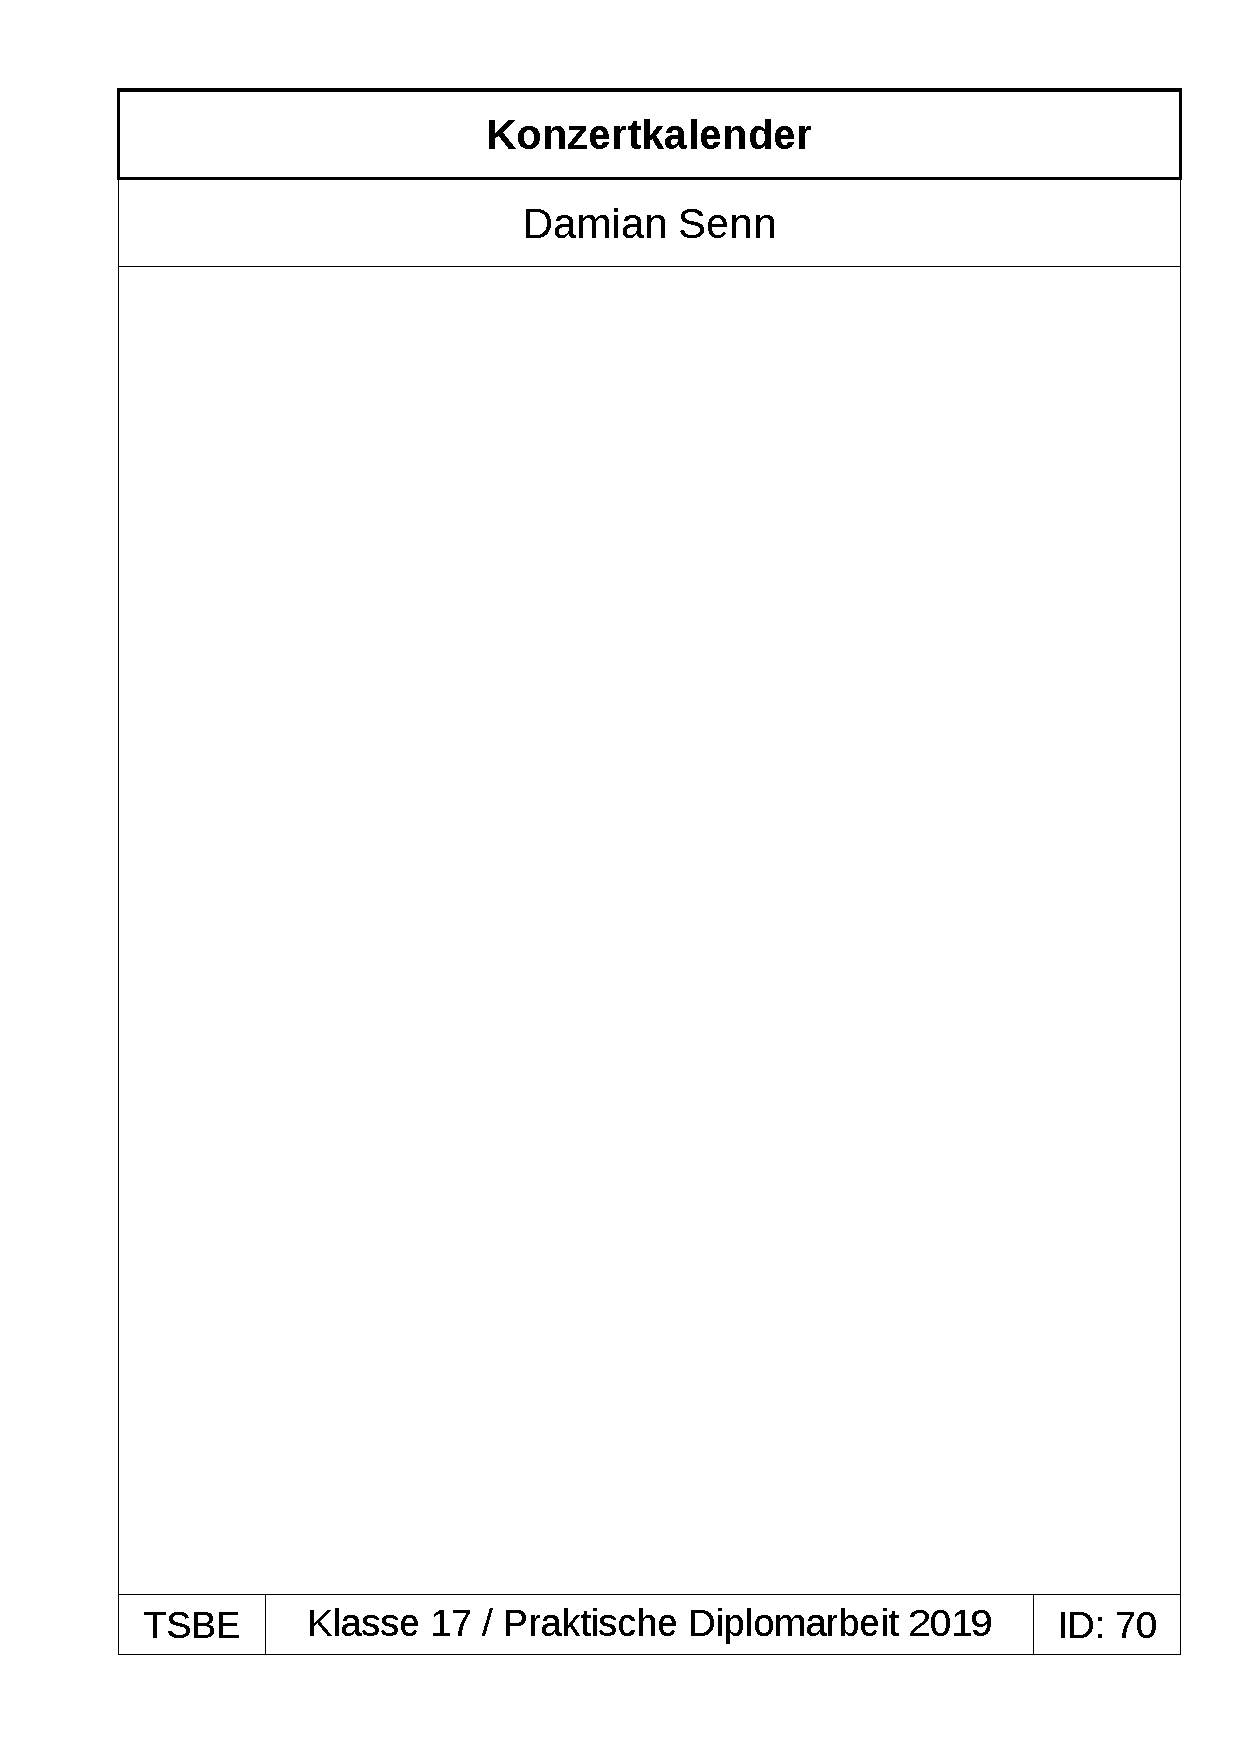
\includepdf[trim=10mm 0mm 0mm 0mm, clip]{titelblatt.pdf}
\begin{titlepage}
  \begin{center}

    \vspace*{.06\textheight}
    {\scshape\LARGE \univname\par}\vspace{1.5cm} % University name
    \textsc{\Large Diplomarbeit}\\[0.5cm] % Thesis type

    \HRule \\[0.4cm] % Horizontal line
    {\huge \bfseries \ttitle\par}\vspace{0.4cm} % Thesis title
    \HRule \\[1.5cm] % Horizontal line

    \begin{minipage}[t]{0.4\textwidth}
      \begin{flushleft} \large
        \emph{Author:}\\
        \href{mailto:damian.senn@gmail.com}{\authorname} % Author name - remove the \href bracket to remove the link
      \end{flushleft}
    \end{minipage}
    \begin{minipage}[t]{0.4\textwidth}
      \begin{flushright} \large
        \emph{Experten:} \\
        \href{mailto:sandro@bertolino.ch}{\supname}\\
        \href{mailto:raez@puzzle.ch}{Severin Räz}
      \end{flushright}
    \end{minipage}\\[3cm]

    \vfill

    \large \textit{Eine Diplomarbeit für den Abschluss \degreename}\\[0.3cm] % University requirement text

    \vfill

    {\large \today}\\[4cm] % Date
    %\includegraphics{Logo} % University/department logo - uncomment to place it

    \vfill
  \end{center}
\end{titlepage}

%------------------------------------------------------------------------------
% DECLARATION PAGE
%------------------------------------------------------------------------------

\begin{declaration}
  \addchaptertocentry{\authorshipname} % Add the declaration to the table of contents
  \noindent Mit meiner Unterschrift bestätige ich, die vorliegende Diplomarbeit
  selbstständig, ohne Hilfe Dritter und nur unter Benutzung der angegebenen
  Quellen ohne Copyright-Verletzung, erstellt zu haben.\\

  \noindent Unterschrift:\\
  \rule[0.5em]{25em}{0.5pt}

  \noindent Ort:\\
  \rule[0.5em]{25em}{0.5pt}

  \noindent Datum:\\
  \rule[0.5em]{25em}{0.5pt}
\end{declaration}

\cleardoublepage

%------------------------------------------------------------------------------
% ABSTRACT PAGE
%------------------------------------------------------------------------------

\renewcommand{\abstractname}{Management Summary}
\begin{abstract}
  \addchaptertocentry{\abstractname} % Add the abstract to the table of contents
  Inhalt für Management Summary folgt hier\ldots
\end{abstract}

%------------------------------------------------------------------------------
% ACKNOWLEDGEMENTS
%------------------------------------------------------------------------------

\begin{acknowledgements}
  \addchaptertocentry{\acknowledgementname} % Add the acknowledgements to the table of contents
  TODO
\end{acknowledgements}

%------------------------------------------------------------------------------
% LIST OF CONTENTS/FIGURES/TABLES PAGES
%------------------------------------------------------------------------------

\tableofcontents % Prints the main table of contents

\listoffigures % Prints the list of figures

\listoftables % Prints the list of tables

%------------------------------------------------------------------------------
% ABBREVIATIONS
%------------------------------------------------------------------------------

\begin{abbreviations}{ll}

  \textbf{HTML} & \textbf{H}yper\textbf{t}ext \textbf{M}arkup \textbf{L}anguage\\
  \textbf{CSS} & \textbf{C}ascading \textbf{S}yle \textbf{S}heets\\
  \textbf{SEO} & \textbf{S}earch \textbf{E}ngine \textbf{O}ptimization\\

\end{abbreviations}

%------------------------------------------------------------------------------
% DEDICATION
%------------------------------------------------------------------------------

\dedicatory{For/Dedicated to/To my\ldots}

%------------------------------------------------------------------------------
% CHAPTERS
%------------------------------------------------------------------------------

\mainmatter % Begin numeric (1,2,3...) page numbering

\pagestyle{thesis} % Return the page headers back to the "thesis" style

% Include the chapters of the thesis as separate files from the Chapters folder
% Uncomment the lines as you write the chapters

\chapter{Initialisierung}

\label{ReportInitialisierung}

\section{Ausgangslage}

\section{Projektziele}

\begin{longtable}[]{@{}lll@{}}
  \toprule
  Nr.  & Zielbeschreibung                                                                       & Muss/Kann\tabularnewline
  \toprule
       & Produktziele\tabularnewline
  \midrule
  1.1  & Besucher können im Produkt nach Konzerten suchen                                       & Muss\tabularnewline
  1.2  & Suchresultate können nach Musik-Genre und Ort gefiltert werden                         & Muss\tabularnewline
  1.3  & Das Produkt soll ein modernes responsives Design vorweisen                             & Muss\tabularnewline
  1.4  & Konzerte sollen von Suchmaschinen indexiert werden können                              & Muss\tabularnewline
  1.5  & Benutzer können isch im Produkt registrieren                                           & Muss\tabularnewline
  1.6  & Benutzer können ihr Passwort nach Verlust neu setzen                                   & Muss\tabularnewline
  1.7  & Inhalte des Portals sind durch die Benutzer erfassbar und bearbeitbar                  & Muss\tabularnewline
  1.8  & Kompatibilität mit aktuellem Google Chrome und Mozilla Firefox Browser                 & Muss\tabularnewline
  1.9  & Konzerte können vom Produkt nach Facebook exportiert werden                            & Kann\tabularnewline
  1.10 & Ein angemeldeter Benutzer kann vermerken ob er einem Konzert teilnimmt                 & Kann\tabularnewline
  1.11 & Das Produkt soll sich an Security Best-Practices von OWASP halten                      & Muss\tabularnewline
  \bottomrule
       & Abwicklungsziele\tabularnewline
  \midrule
  2.1  & \makecell[l]{Das Projekt soll nach HERMES 5 unter Berücksichtigung der Richtlinien von                            \\ der TSBE dokumentiert werden} & Muss\tabularnewline
  2.2  & Das Produkt muss bis Projektende fertiggestellt und bereit für die Einführung sein     & Muss\tabularnewline
  2.3  & Die Technische-Umsetzung wird durch Damian Senn erstellt                               & Muss\tabularnewline
  2.4  & \makecell[l]{Die Kommunikation zwischen Experten und Diplomanden erfolgt wie im                                   \\ Projektauftrag \ref{kommunikation} beschrieben.} & Muss\tabularnewline
  2.5  & Das Projekt muss bis Ende Mai 2019 abgeschlossen sein                                  & Muss\tabularnewline
  \bottomrule
\end{longtable}


\clearpage

\section{Projektorganisation}

\begin{figure}[!htb]
  \centering
  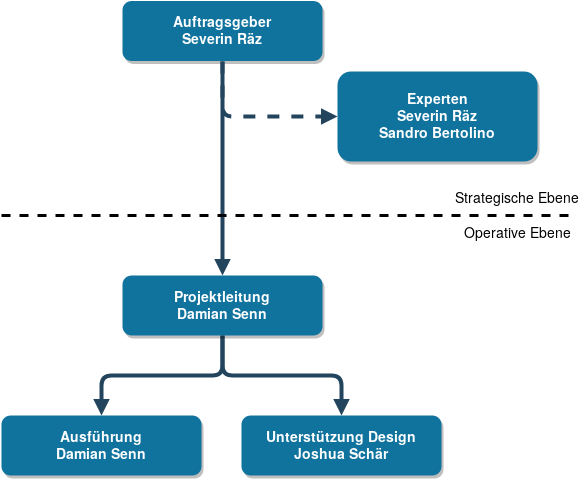
\includegraphics[width=0.8\textwidth]{figures/organigram.png}
  \caption{Organigram}
\end{figure}

\section{Projektplan}

\section{Lieferergebnisse}

\section{Ressourcenplan}

\section{Risiken}

\clearpage

\section{Abgrenzungen}

\begin{figure}[!htb]
  \centering
  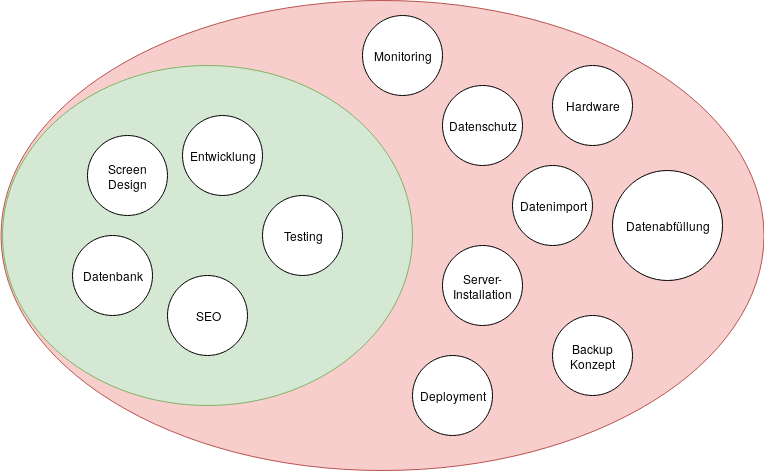
\includegraphics[width=0.95\textwidth]{figures/abgrenzungen.png}
  \caption{Abgrenzungen}
\end{figure}

Die detaillierten Erklärung zu den Abgrenzungen sind im Projektauftrag~\ref{abgrenzungen} zu finden.

\clearpage

\section{Studie}

\subsection{Informationsbeschaffung}

\subsection{Anforderungskatalog}

\subsection{Pflichtenheft}

\subsection{Mögliche Varianten}

\subsection{Evaluation Varianten}

\subsection{Entscheid Varianten}

\subsection{Wirtschaftlichkeit}

\chapter{Konzept}

\label{AppendixKonzept}

\section{Zweck des Dokuments}\label{KonzeptZweck}

Das Konzept dient als Anleitung für die Realisierungsphase. Die in der Konzept
erarbeiteten Details müssen in der Realisierung eingehalten un umgesetzt
werden.

\subsection{Teilkonzepte}

Durch die in der Studie gewonnenen Erkentnissen, werden in der Phase Konzept
verschiedene Teilkonzepte erstellt.

Im Teilkonzept «Portalname» wird der Name des Produktes erarbeitet.

Im Teilkonzept «Design- und Bedienkonzept» werden die Ansichten der Applikation
in Mockups umgesetzt. Es werden die Benutzer Use-Cases vom Besucher sowie der
Konzert-Erfasser aufgezeigt.

Im Teilkonzept «Softwarekonzept» werden die Datenflüsse hinter den Mockups
aufgezeigt, sowie die Datenbankstruktur aufgebaut.

Im Teilkonzept «Testkonzept» werden die einzelnen Systemtests aufgelistet sowie
ausgearbeitet wie granular welche Teile der Software getestet werden sollen.

Im letzten Teil des Konzept-Dokuments wird im Fazit dokumentiert, wie und warum
das Konzept von den vorhergehenden Phasen des Projekts abweicht.


\clearpage
\section{Portalname}\label{portalname}

Der Portalname wurde in einer Brainstorming-Session von Damian Senn auf
den Namen \textbf{«Gigpillar»} festgelegt. Der Name ist angelehnt an die Werbepfeiler in
Städten, wo oft Werbeplakate für Konzerte hängen.

Die folgenden Ideen wurden in Betracht gezogen, jedoch war keine Domain mehr
verfügbar oder der Name überzeugte nicht:

\begin{itemize}
  \item{} upto.com («What are you up to?»)
  \item{} up-to.com
  \item{} uptoin.com
  \item{} gigup.com
  \item{} gigsta.com («Gigs to attend»)
  \item{} gigin.com
  \item{} gigsin.com
  \item{} gixin.com («Gigs in»)
  \item{} dualact.com («Loud act»)
  \item{} trecnoc.com («Concert» rückwärts)
\end{itemize}

\clearpage
\section{Design- und Bedienkonzept}\label{design--und-bedienkonzept}

\subsection{Mockups}

\subsubsection{Homepage}

Die Homepage ist die erste Seite, die der Besucher sieht, wenn er/sie die
Applikation direkt über \href{https://gigpillar.com/}{gigpillar.com} aufruft.
Auf den ersten Blick ist die Suche sowie ein grosses Bild (Banner) eines Gigs
zu erblicken. Weiter sind Links zu gängigen Funktionalitäten wie Gig hinzufügen
sowie das Login in einer Navigation erreichbar.

Unter dem Banner werden Gigs in nächster nähe des Besuchers aufgelistet, der
Link «change location» führt weiter zur Suchresultate Seite um den
entsprechenden Filter anzupassen.

\begin{figure}[!htb]
  \centering
  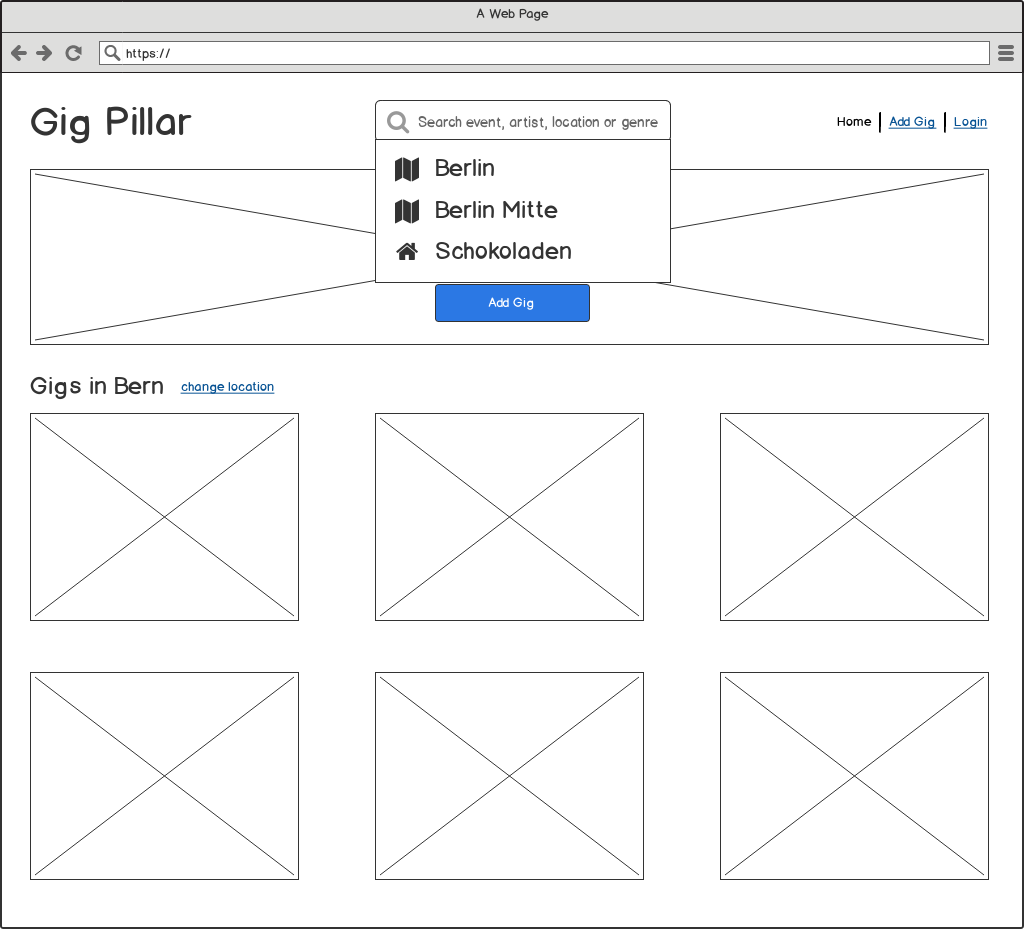
\includegraphics[width=0.95\textwidth]{mockups/homepage.png}
  \caption{Mockup: Homepage}
\end{figure}

\clearpage
\subsubsection{Suchresultate}

Auf der Suchresultate Seite sieht der Benutzer seine Suchresultate der von der
globalen Suchbox ausgelösten Suche. Die Seite bietet weitere Filter an um die
Resultate weiter einzugrenzen.\\

\noindent
Folgende Filter stehen den Benutzern zur Verfügung:

% TODO: This diverges from our search criteria described in the previous phase.

\begin{itemize}
  \tightlist{}
  \item{} Ort
  \item{} Datum von
  \item{} Datum bis
  \item{} Musik Genre
\end{itemize}

\noindent
Das Anwählen eines Suchresultates führt den Benutzer weiter zur detaillierten
Gig Ansicht.

\begin{figure}[!htb]
  \centering
  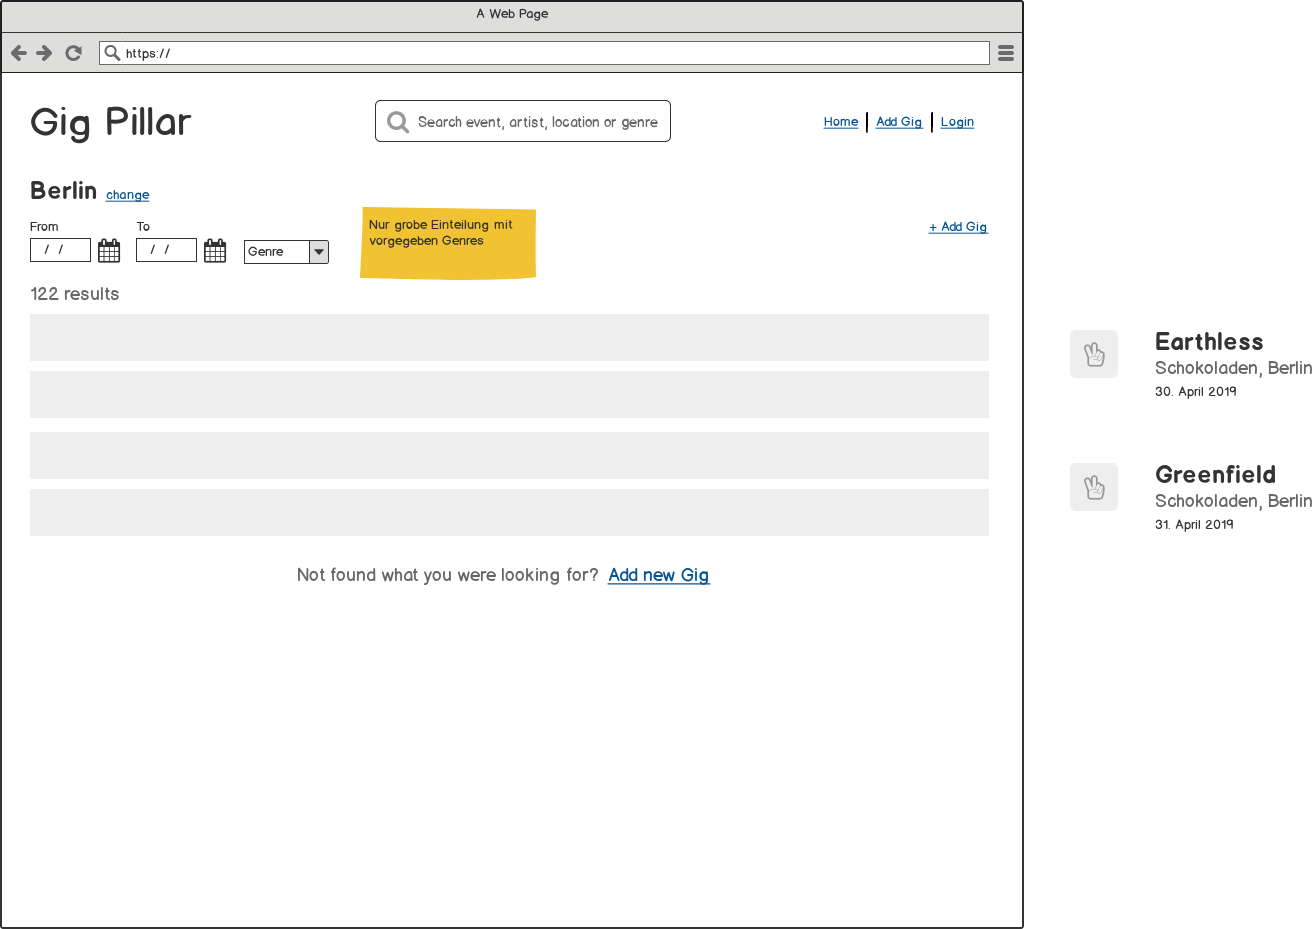
\includegraphics[width=0.95\textwidth]{mockups/search-result.png}
  \caption{Mockup: Suchresultate}
\end{figure}

\clearpage
\subsubsection{Gig Ansicht}

In der Gig Ansicht werden alle Details zu einem Event aufgelistet.

\begin{itemize}
  \tightlist{}
  \item{} Datum des Events
  \item{} Zeit wann das Event beginnt, bzw die Location die Türen öffnet
  \item{} Liste aller Künstler mit optionaler Startzeit
  \item{} Eine Beschreibung des Events
  \item{} Die Adresse der Location mit Link auf Google Maps
\end{itemize}

\noindent
Ausserdem soll es den Benutzern möglich sein, über einen «Add to my calendar»
Link das Event zu seiner Kalender-Applikation zu importieren.

\begin{figure}[!htb]
  \centering
  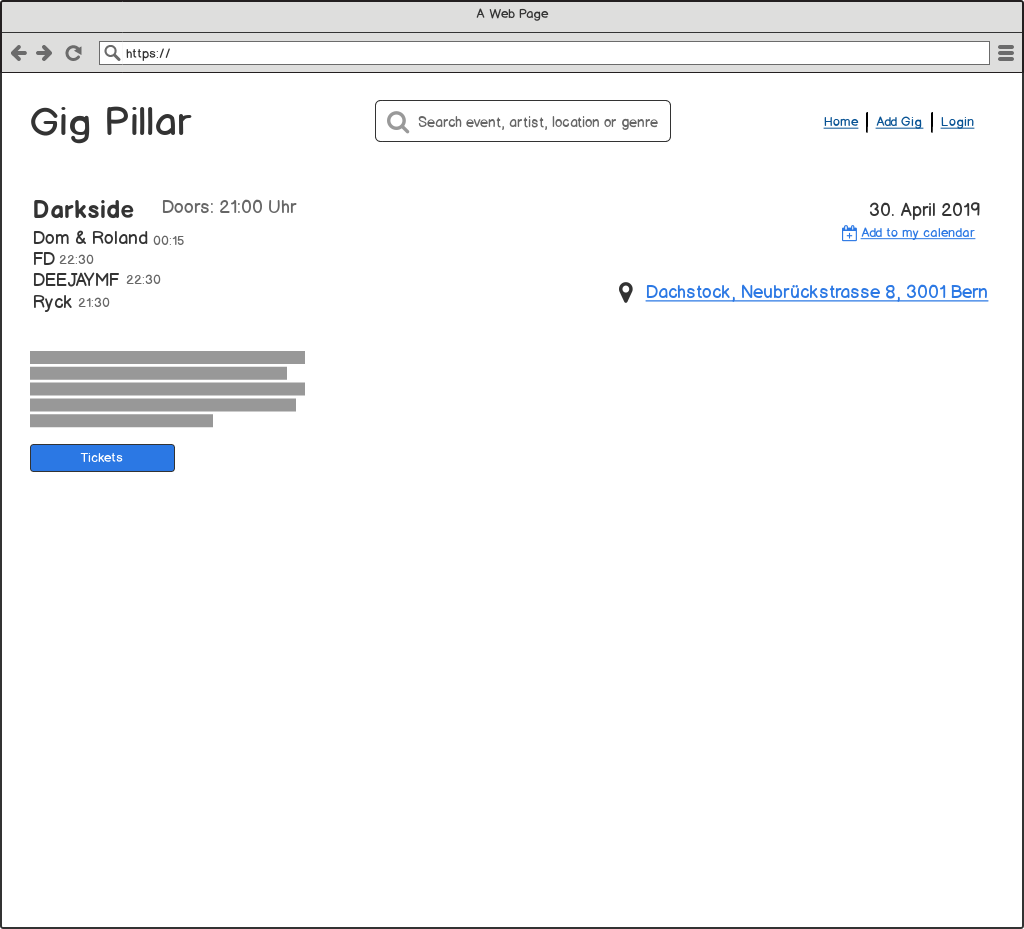
\includegraphics[width=0.95\textwidth]{mockups/event.png}
  \caption{Mockup: Gig Ansicht}
\end{figure}

\clearpage
\subsubsection{Gig erfassen}

Benutzer können Gigs erfassen.\\

\noindent
Folgende Daten sind für einen Gig zu erfassen:

\begin{itemize}
  \tightlist{}
  \item{} Name
  \item{} Bild \textit{(optional)}
  \item{} Location
  \item{} Datum
  \item{} Zeit
  \item{} Eine Liste von Artists mit optionaler Startzeit
  \item{} Beschreibung
  \item{} Link zum Ticketvertreiber
\end{itemize}

\begin{figure}[!htb]
  \centering
  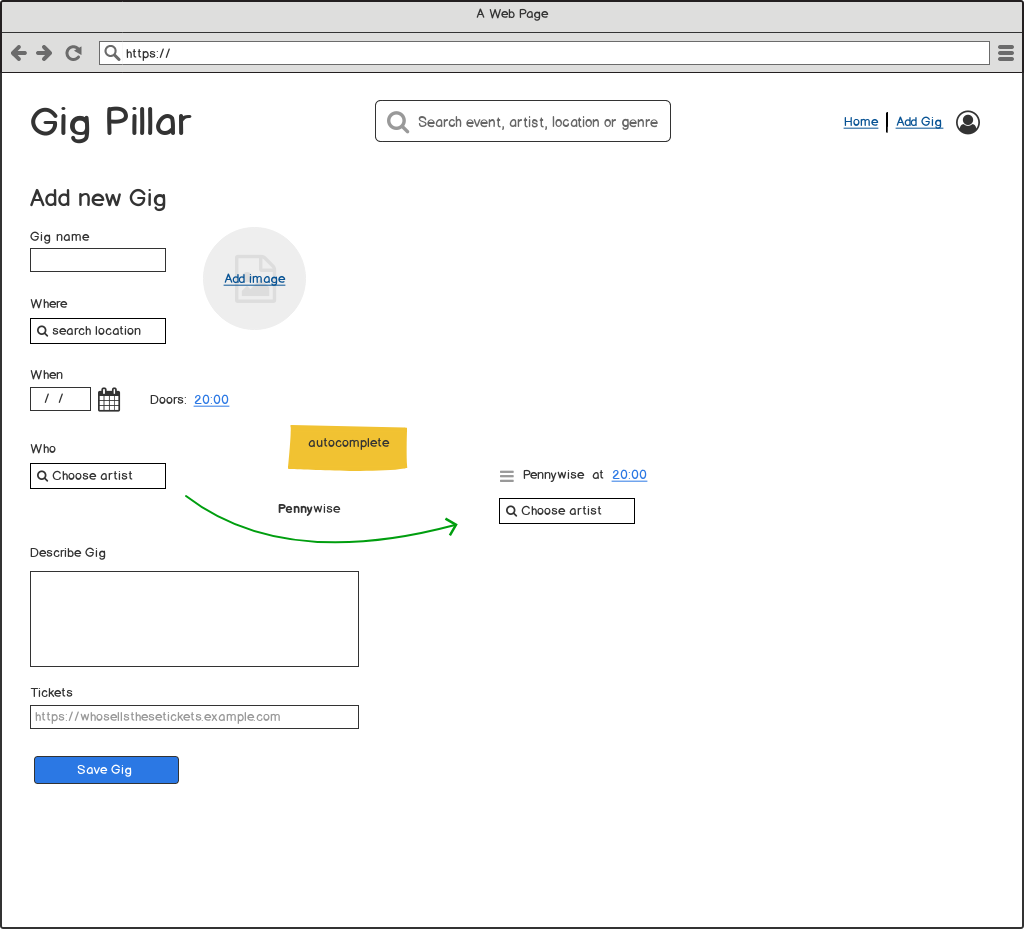
\includegraphics[width=0.95\textwidth]{mockups/add-gig.png}
  \caption{Mockup: Gig erfassen}
\end{figure}

\clearpage
\subsubsection{Benutzerprofil}

Benutzer können ihr eigenes Profil verwalten und folgende Tätigkeiten
verrichten:

\begin{itemize}
  \tightlist{}
  \item{} Anzeigename ändern
  \item{} E-Mail Adresse ändern \textit{(mit E-Mail Bestätigung)}
  \item{} Passwort ändern \textit{(muss vorher altes Passwort bestätigen)}
  \item{} Account löschen \textit{(muss doppelt bestätigt werden!)}
\end{itemize}

\begin{figure}[!htb]
  \centering
  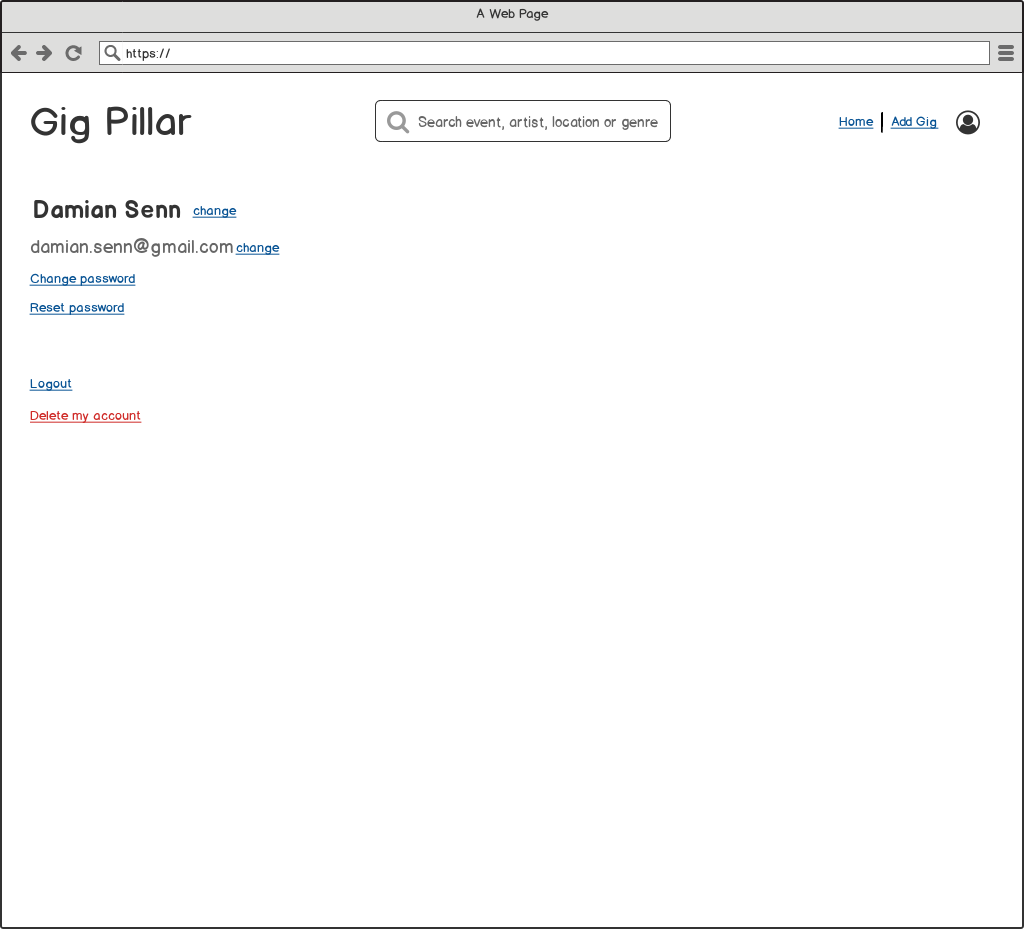
\includegraphics[width=0.95\textwidth]{mockups/profile.png}
  \caption{Mockup: Benutzerprofil}
\end{figure}

\clearpage
\subsection{Genre Filter}\label{genrefilter}

Der Genre Filter soll folgende Werte zur Verfügung stellen.

\begin{itemize}
  \item{} Alternative
  \item{} Blues
  \item{} Classical
  \item{} EDM
  \item{} Hip-Hop
  \item{} Jazz
  \item{} Metal
  \item{} Pop
  \item{} Punk
  \item{} Reggae
  \item{} Rock
\end{itemize}

\clearpage
\section{Softwarekonzept}\label{softwarekonzept}
\subsection{Datenfluss}\label{datenfluss}

\subsubsection{Homepage}\label{datenfluss-homepage}

Die Homepage zeigt den Besuchern Gigs in ihrer Nähe an, dazu muss über eine
GeoIP API die IP-Adresse des Besuchers auf ein Land zurückverfolgt werden.
Dazu wird beim ersten Besuch die GeoIP API abgefragt und das Land des Benutzers
in eine Session geschrieben. Bei weiteren Aufrufen wird das Land direkt aus der
Session bezogen.

%GigPillarWeb
%GigPillarWeb_Session
%GigPillar
%GeoIp
%
%Response = GigPillarWeb./ {
%  if (hasSession) {
%    location = GigPillarWeb_Session.getLocation()
%  } else {
%    location = GigPillarWeb_Session.createSession() {
%      location = GeoIp.getLocation(ip)
%    }
%  }
%
%  Events = GigPillar.getUpcomingEvents(location)
%}

\begin{figure}[!htb]
  \centering
  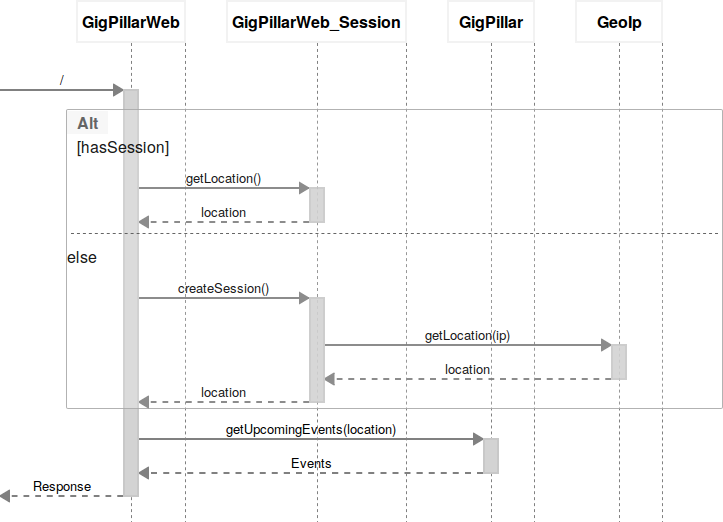
\includegraphics[width=0.95\textwidth]{konzept/datenfluss-homepage.png}
  \caption{Datenfluss: Homepage}
\end{figure}

\clearpage
\subsubsection{Suchfeld}\label{datenfluss-suchfeld}

Das globale Suchfeld hat eine Autocompletion, welche Daten direkt von
der GigPillar Applikation bezieht. Die Daten für Städtenamen wird jedoch von
einer externen Datenquelle, z.B. Google Maps, bezogen.

%GigPillarWeb
%GigPillar
%GoogleMaps
%
%Response = GigPillarWeb./searchCompletion {
%  Cities = GoogleMaps.searchCities(searchParameters)
%  Locations = GigPillar.searchLocations(searchParameters)
%  Genres = GigPillar.searchGenres(searchParameters)
%  Artists = GigPillar.searchArtists(searchParameters)
%  Events = GigPillar.searchEvents(searchParameters)
%}

\begin{figure}[!htb]
  \centering
  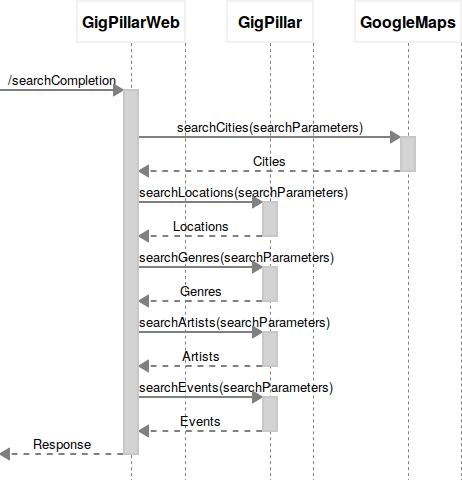
\includegraphics[width=0.95\textwidth]{konzept/datenfluss-suchfeld.png}
  \caption{Datenfluss: Suchfeld}
\end{figure}

\clearpage
\subsubsection{Gig erstellen - Locationfeld}\label{datenfluss-gig-erstellen-locationfeld}

Beim Erstellen eines neuen Gigs, muss eine Location zugewiesen werden. Die
Locations werden über die bereits in GigPillar erfassten Locations sowie über
eine externe Datenquelle, wie z.B. Google Maps, bezogen.

%GigPillarWeb
%GigPillar
%GoogleMaps
%
%Response = GigPillarWeb./locationCompletion {
%  Locations = GigPillar.searchLocations(searchParameters) {
%    Locations = searchLocations(searchParameters)
%    Locations = GoogleMaps.searchLocations(searchParameters)
%  }
%}

\begin{figure}[!htb]
  \centering
  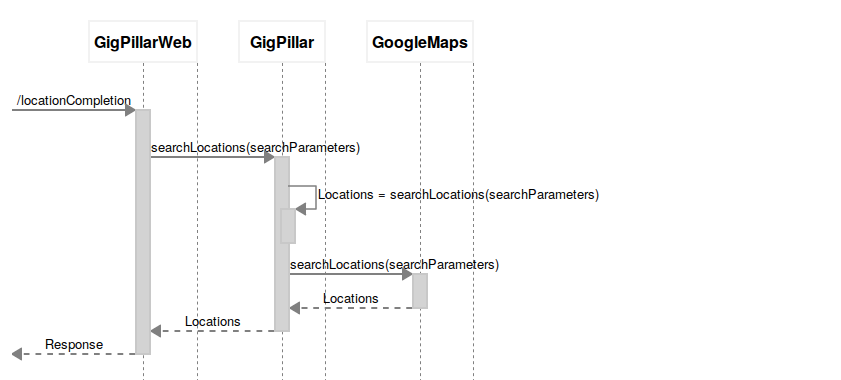
\includegraphics[width=0.95\textwidth]{konzept/datenfluss-locationfeld.png}
  \caption{Datenfluss: Gig erstellen - Locationfeld}
\end{figure}

%TODO:
%\clearpage
%\subsubsection{Gig erstellen}\label{datenfluss-gigerstellen}

\clearpage
\subsubsection{Passwort-Reset}\label{datenfluss-passwort-reset}

Falls ein Benutzer sein Passwort vergessen hat, kann dieser ein neues Passwort
über die Passwort-Reset Funktion setzen. Beim Auslösen eines Passwort-Resets,
wird dem Benutzer ein E-Mail mit einem Link zugeschickt.
Der Passwort-Reset-Link führt den Benutzer auf ein Formular auf welchem er/sie
die Möglichkeit hat, ein neues Passwort zu setzen.

%GigPillarWeb
%GigPillar
%UserEmailClient
%
%Response = GigPillarWeb./passwordReset {
%  GigPillar.sendPasswordResetEmail(email) {
%    GigPillar->UserEmailClient:SMTP
%  }
%}
%
%Redirect = UserEmailClient.clickPasswordResetLink {
%  Response = GigPillarWeb./passwordRestToken
%}
%
%Response = GigPillarWeb./setPassword {
%  GigPillar.setUserPassword(currentUser, password)
%}

\begin{figure}[!htb]
  \centering
  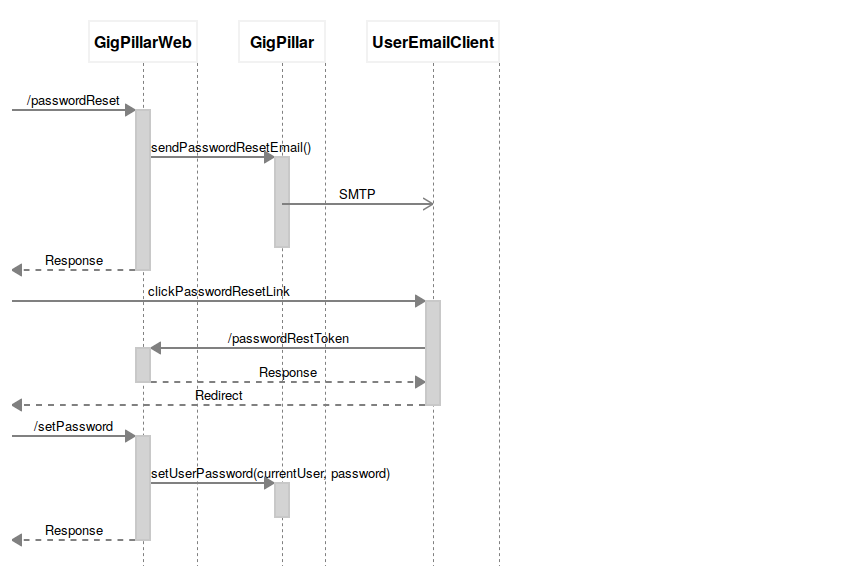
\includegraphics[width=0.95\textwidth]{konzept/datenfluss-passwort-reset.png}
  \caption{Datenfluss: Passwort-Reset}
\end{figure}

\clearpage
\subsection{Datenbankstruktur}\label{datenbankstruktur}

\begin{figure}[!htb]
  \centering
  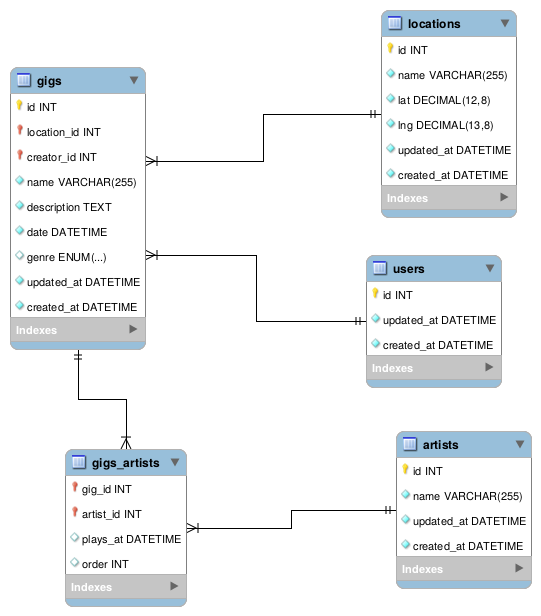
\includegraphics[width=0.95\textwidth]{konzept/erd.png}
  \caption{Entity Relationship Diagram}
\end{figure}

\clearpage
\section{Testkonzept}\label{testkonzept}

\subsection{Unit-Tests}\label{unittests}

% Do ~80% code coverage

\subsection{Visual-Tests}\label{visualtests}

% Do simple screenshot diffing for every screen

\clearpage
\subsection{Akzeptanztests}\label{akzeptanztests}

% TODO: Akzeptanztest basieren auf Anforderungen

\newcounter{acceptancetest}

\NewDocumentCommand{\acceptancetest}{
  O{}
  O{}
  O{\tabularnewline\tabularnewline}
  O{\tabularnewline\tabularnewline\tabularnewline\tabularnewline}
  m
  m
}{
  \begin{longtable}[]{@{}l|p{6cm}p{4cm}@{}}
    \toprule
    \stepcounter{acceptancetest}
    \textbf{Test \arabic{acceptancetest}} & \textbf{Tester:} #1 & \textbf{Datum:} #2 \tabularnewline
    \midrule
    \textbf{Kriterium}                    & \multicolumn{2}{p{10cm}}{#5}\tabularnewline
    \textbf{Erwartetes Ergebnis}          & \multicolumn{2}{p{10cm}}{#6}\tabularnewline
    \midrule
    \textbf{Testergebnis}                 & #3\tabularnewline
    \midrule
    \textbf{Fehlerbeschreibung}           & #4\tabularnewline
    \bottomrule
    \caption{Akzeptanztest \arabic{acceptancetest}}
  \end{longtable}
}

\acceptancetest
  {Es ist möglich nach Konzerten in einem bestimmten Ort zu suchen.}
  {Nach auswählen von «Berlin» in der Suche, werden nur noch Konzerte in Berlin aufgelistet.}

\acceptancetest
  {Es ist möglich eine Suche weiter nach Genre einzuschränken.}
  {Nach auswählen von «Rock» in einem Suchresultat, werden nur noch Rock-Konzerte aufgelistet.}

\clearpage

\acceptancetest
  {Responsive - Homepage}
  {Sieht auf Desktop, Tablet und Mobile gut aus und stellt jeweils alle relevanten Daten dar.}

\acceptancetest
  {Browserkompatibilität - Homepage}
  {Funktioniert in den unterstützten Browsern.}

\clearpage

\acceptancetest
  {Responsive - Suche}
  {Sieht auf Desktop, Tablet und Mobile gut aus und stellt jeweils alle relevanten Daten dar.}

\acceptancetest
  {Browserkompatibilität - Suche}
  {Funktioniert in den unterstützten Browsern.}

\clearpage

\acceptancetest
  {Responsive - Gig Ansicht}
  {Sieht auf Desktop, Tablet und Mobile gut aus und stellt jeweils alle relevanten Daten dar.}

\acceptancetest
  {Browserkompatibilität - Gig Ansicht}
  {Funktioniert in den unterstützten Browsern.}

\clearpage

\acceptancetest
  {Responsive - Login}
  {Sieht auf Desktop, Tablet und Mobile gut aus und stellt jeweils alle relevanten Daten dar.}

\acceptancetest
  {Browserkompatibilität - Login}
  {Funktioniert in den unterstützten Browsern.}

\clearpage

\acceptancetest
  {Responsive - Registrierung}
  {Sieht auf Desktop, Tablet und Mobile gut aus und stellt jeweils alle relevanten Daten dar.}

\acceptancetest
  {Browserkompatibilität - Registrierung}
  {Funktioniert in den unterstützten Browsern.}

\clearpage

\acceptancetest
  {Responsive - Gig erfassen}
  {Sieht auf Desktop, Tablet und Mobile gut aus und stellt jeweils alle relevanten Daten dar.}

\acceptancetest
  {Browserkompatibilität - Gig erfassen}
  {Funktioniert in den unterstützten Browsern.}

\clearpage

\acceptancetest
  {Gig erfassen}
  {Folgende Daten können erfasst werden:
  \begin{itemize}
    \tightlist{}
    \item{} Name
    \item{} Bild
    \item{} Location
    \item{} Datum
    \item{} Zeit
    \item{} Künstler mit optinaler Start-Zeit
    \item{} Beschreibung
    \item{} Link zum Ticketvertreiber
  \end{itemize}}

\acceptancetest
  {Neue Gigs tauchen in der Suche auf.}
  {Der neu erstellte Gig taucht in der Suche auf.}

\clearpage

\acceptancetest
  {Responsive - Benutzerprofil}
  {Sieht auf Desktop, Tablet und Mobile gut aus und stellt jeweils alle relevanten Daten dar.}

\acceptancetest
  {Browserkompatibilität - Benutzerprofil}
  {Funktioniert in den unterstützten Browsern.}

\clearpage

\acceptancetest
  {Responsive - Passwort-Reset}
  {Sieht auf Desktop, Tablet und Mobile gut aus und stellt jeweils alle relevanten Daten dar.}

\acceptancetest
  {Browserkompatibilität - Passwort-Reset}
  {Funktioniert in den unterstützten Browsern.}

\clearpage

\acceptancetest
  {Security - Suche}
  {Das Suchfeld ist resistent gegen XSS und SQL-Injection}

\acceptancetest
  {Security - Login}
  {Das Login ist resistent gegen XSS und SQL-Injection}

\clearpage

\acceptancetest
  {Security - Benutzerprofil}
  {Das Benutzerprofil ist resistent gegen XSS und SQL-Injection}

\acceptancetest
  {Security - Gig erfassen}
  {Das Gig erfassen Formular ist resistent gegen XSS und SQL-Injection}

\clearpage
\section{Fazit}\label{konzept-fazit}

\subsection{Probleme}

% Abweichung "Filter-System" in Suche?

\subsection{Machbarkeit}

% Google Maps API?

\subsection{Wirtschaftlichkeit}

% Änderung an Aufwand?

\subsection{Erweiterbarkeit}

% FB Events etc?

\subsection{Projektplan}

\chapter{Realisierung}\label{AppendixRealisierung}

\section{HTML-Prototyp}

Der HTML-Prototyp ist im Verzeichnis «html-prototype» zu finden, dieser wurde
mit \textbf{Ember.js} und \textbf{SASS} umgesetzt.
Um den Prototypen zu starten muss \textbf{Node.js} und \textbf{Yarn} installiert sein.

\noindent
Den Prototypen kann man mit dem folgenden Kommando starten:

\begin{lstlisting}[language=bash,frame=single]
$ yarn && yarn start
\end{lstlisting}

\noindent
Danach kann der Prototyp über die URL \url{http://localhost:4200/} geöffnet werden.

\noindent
Folgende URLs sind verfügbar:

\begin{itemize}
  \tightlist{}
  \item{} \url{http://localhost:4200/}
  \item{} \url{http://localhost:4200/search}
  \item{} \url{http://localhost:4200/gig-detail}
  \item{} \url{http://localhost:4200/add-gig}
  \item{} \url{http://localhost:4200/login}
  \item{} \url{http://localhost:4200/register}
\end{itemize}

\clearpage
\subsection{Screenshots}

\subsubsection{Homepage}

\begin{figure}[!htb]
  \centering
  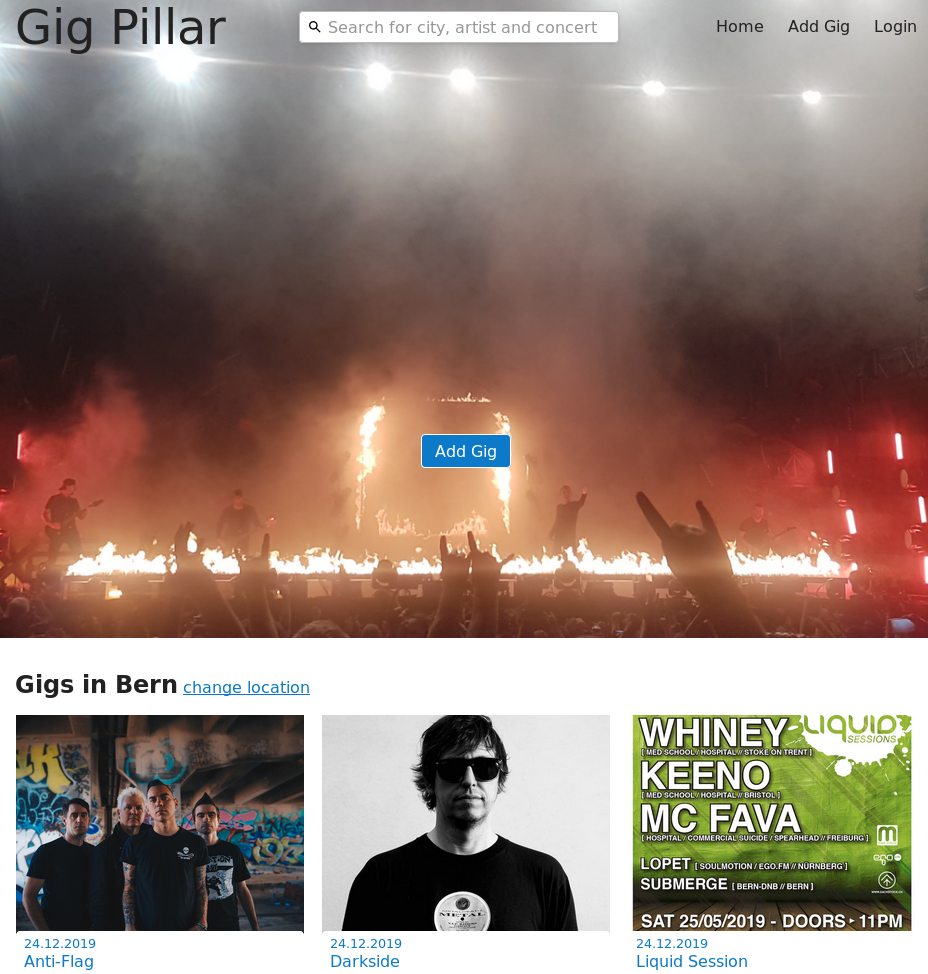
\includegraphics[width=1\textwidth]{figures/html-prototype.png}
  \caption{HTML Prototyp: Homepage}
\end{figure}

\clearpage
\subsubsection{Suche}

\begin{figure}[!htb]
  \centering
  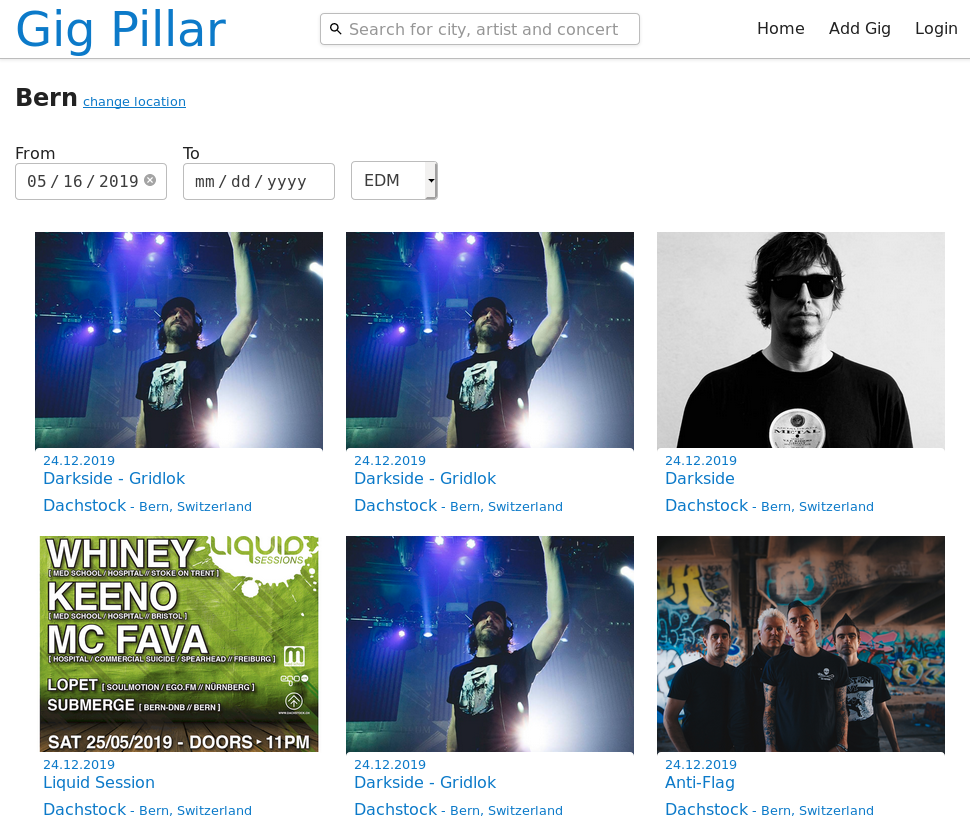
\includegraphics[width=1\textwidth]{realisierung/html-proto-search.png}
  \caption{HTML Prototyp: Suche}
\end{figure}

\clearpage
\subsubsection{Gig erfassen}

\begin{figure}[!htb]
  \centering
  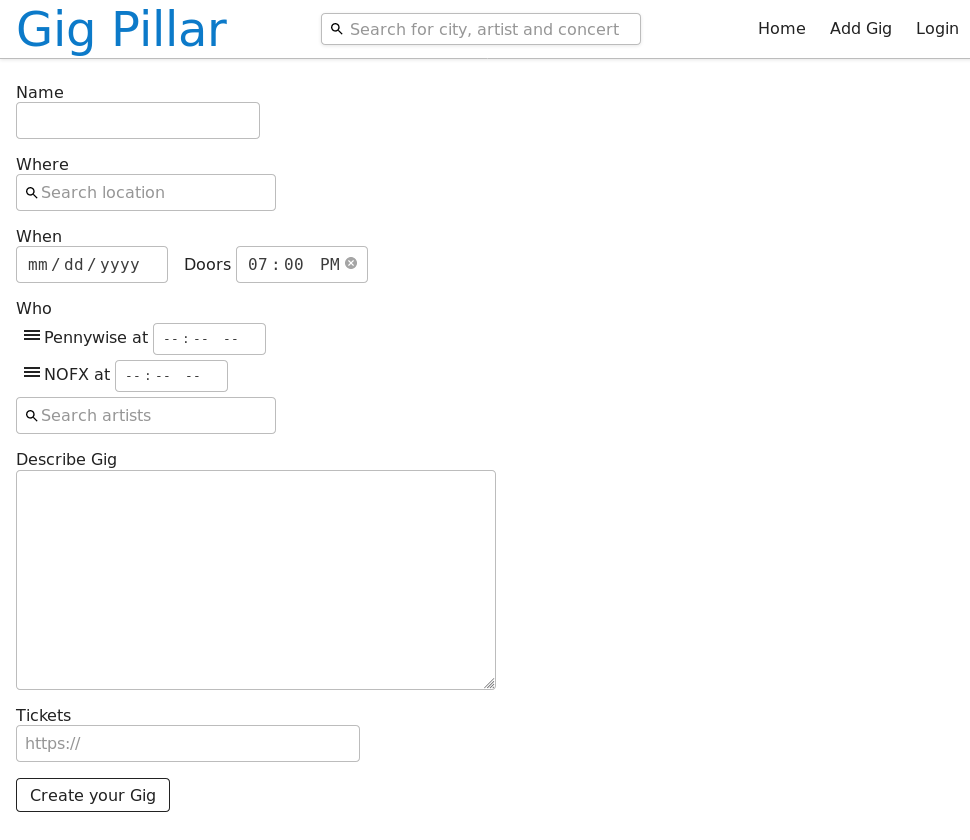
\includegraphics[width=1\textwidth]{realisierung/html-proto-add-gig.png}
  \caption{HTML Prototyp: Gig erfassen}
\end{figure}

\clearpage
\subsubsection{Login}

\begin{figure}[!htb]
  \centering
  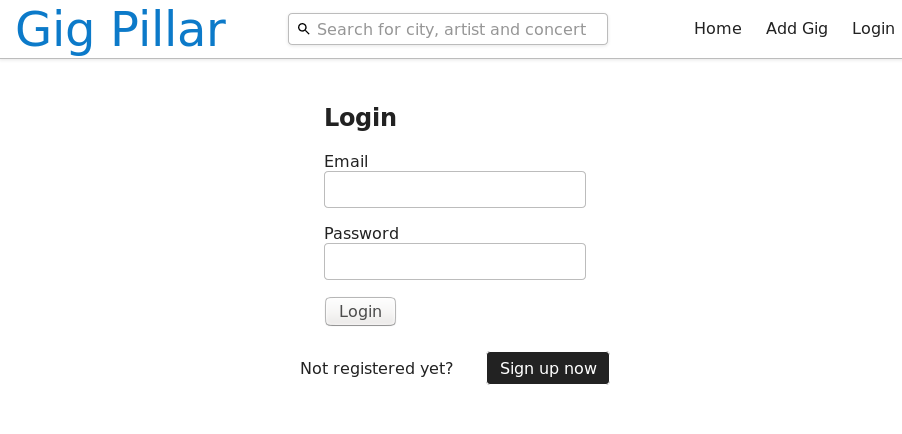
\includegraphics[width=1\textwidth]{realisierung/html-proto-login.png}
  \caption{HTML Prototyp: Login}
\end{figure}

\clearpage
\subsubsection{Registrierung}

\begin{figure}[!htb]
  \centering
  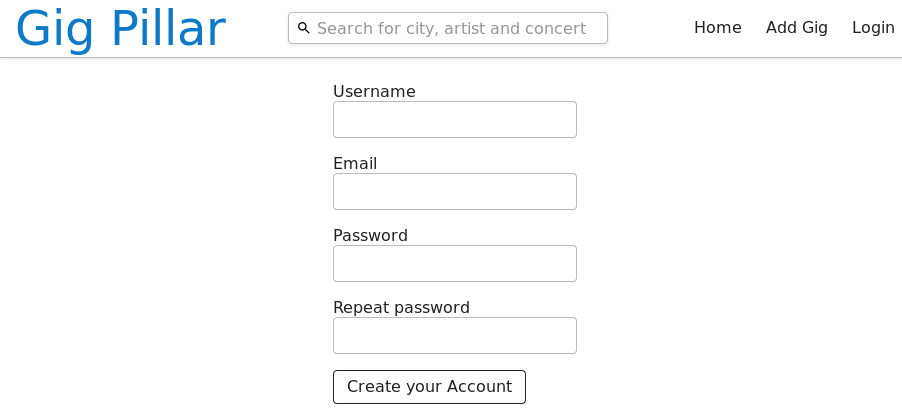
\includegraphics[width=1\textwidth]{realisierung/html-proto-signup.png}
  \caption{HTML Prototyp: Registrierung}
\end{figure}

\clearpage
\section{Projekt Setup}

Die Initialisierung des Projekts wurde mit der Phoenix Framework «Umbrella»
Struktur erstellt.

\begin{lstlisting}[language=bash,frame=single]
$ mix phx.new gigpillar --umbrella
\end{lstlisting}

Die Umbrella Struktur trennt die Applikation in kleinere Teilapplikationen,
dies ermöglicht eine klarere Trennung zwischen der Webapplikation und der Businesslogik.\\
\\
\noindent{}Projektstruktur:
\begin{itemize}
  \tightlist{}
  \item{} \textbf{/apps/}\\Die Phoenix Teilapplikationen
  \item{} \textbf{/apps/gigpillar/}\\Die Gigpillar Grundapplikation
  \item{} \textbf{/apps/gigpillar\_web/}\\Die Gigpillar Webapplikation
  \item{} \textbf{/apps/gigpillar\_web/assets/}\\Der CSS und JavaScript Code für die Webapplikation
  \item{} \textbf{/html-prototype/}\\Der HTML Prototyp
  \item{} \textbf{/doc/}\\Die Projektdokumentation
  \item{} \textbf{/doc/main.pdf}\\Das PDF der Projektdokumentation
\end{itemize}

\clearpage
\section{Dependency Management}

Für das Dependency Management, wurde ein Bot eingerichtet, der
Benachrichtigungen, bzw. Pull-Requests, bei Updates zustellt.

Für das Projekt wurde der Bot «Dependabot»\footnote{\url{https://github.com/marketplace/dependabot}} ausgewählt, da diser Elixir sowie JavaScript Abhängigkeiten unterstützt.

Durch die Benützung des Dependabot, können während der Entwicklung des Projektes
die Software Abhängigkeiten jederzeit auf dem neusten Stand gehalten werden.

\noindent{}Installation von Dependabot:

\begin{figure}[!htb]
  \centering
  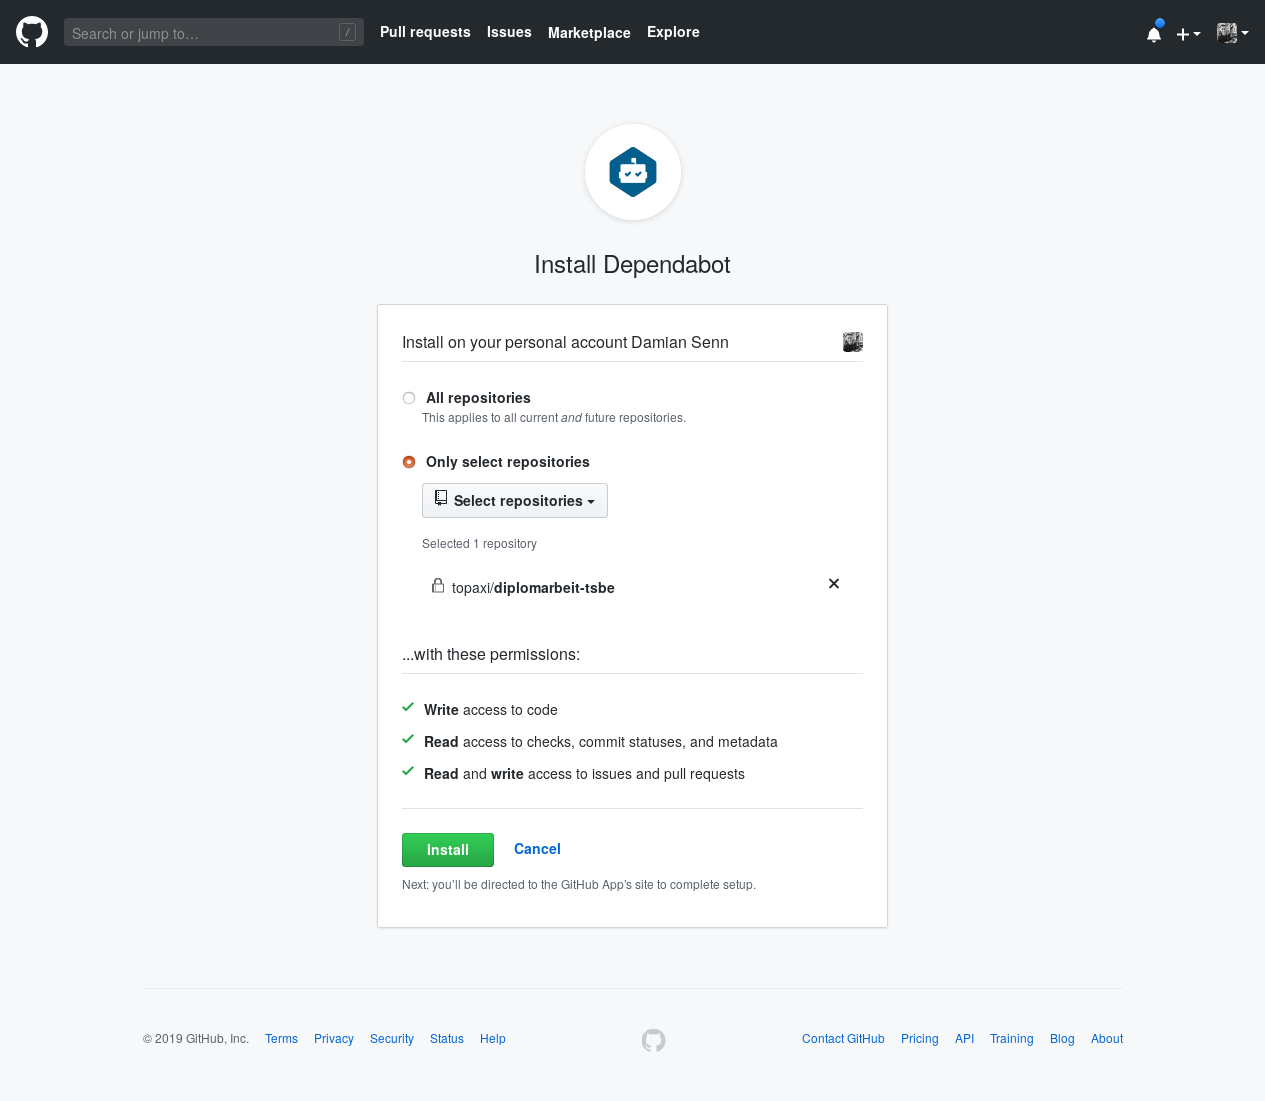
\includegraphics[width=1\textwidth]{realisierung/install-dependabot-1.png}
  \caption{Dependabot: Installation}
\end{figure}

\begin{figure}[!htb]
  \centering
  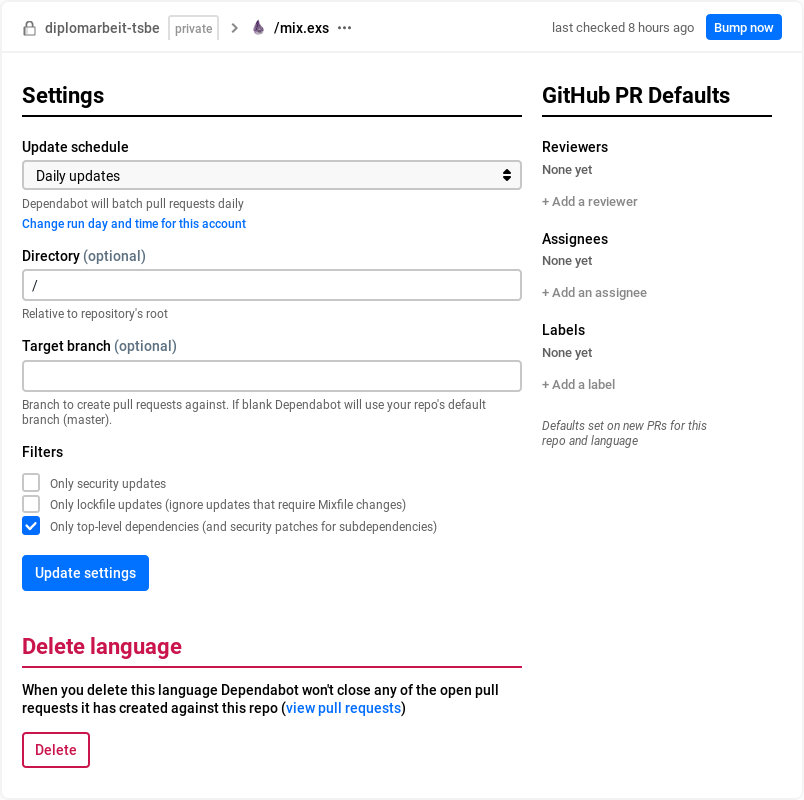
\includegraphics[width=1\textwidth]{realisierung/install-dependabot-2-cropped.png}
  \caption{Dependabot: Konfiguration für Elixir}
\end{figure}

\begin{figure}[!htb]
  \centering
  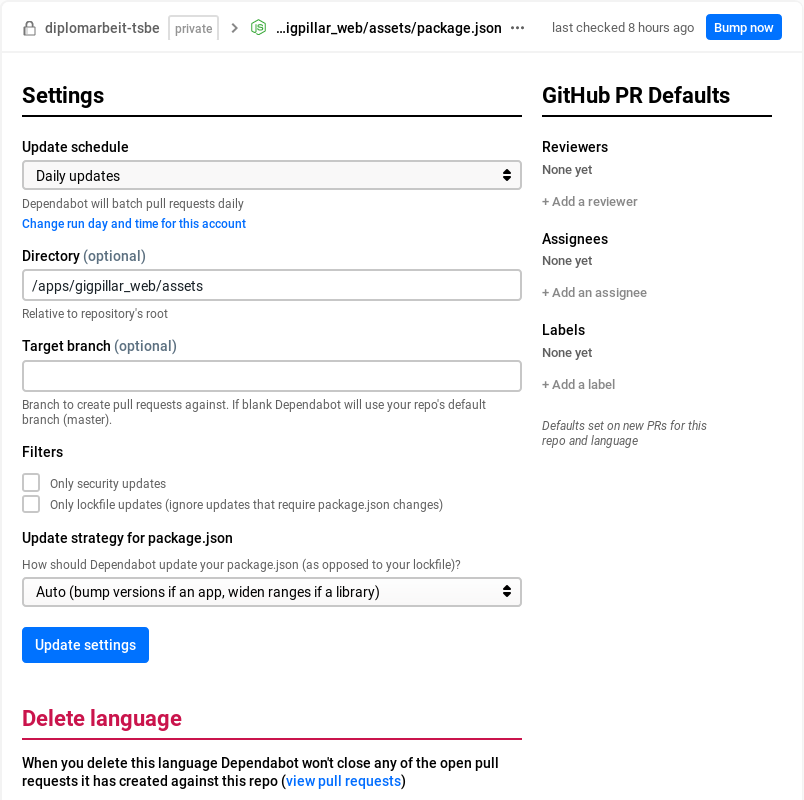
\includegraphics[width=1\textwidth]{realisierung/install-dependabot-3-cropped.png}
  \caption{Dependabot: Konfiguration für JavaScript}
\end{figure}

\clearpage
Diverse Updates konnten via Pull-Requests von Dependabot während der Entwicklung
vorgenommen werden:

\begin{figure}[!htb]
  \centering
  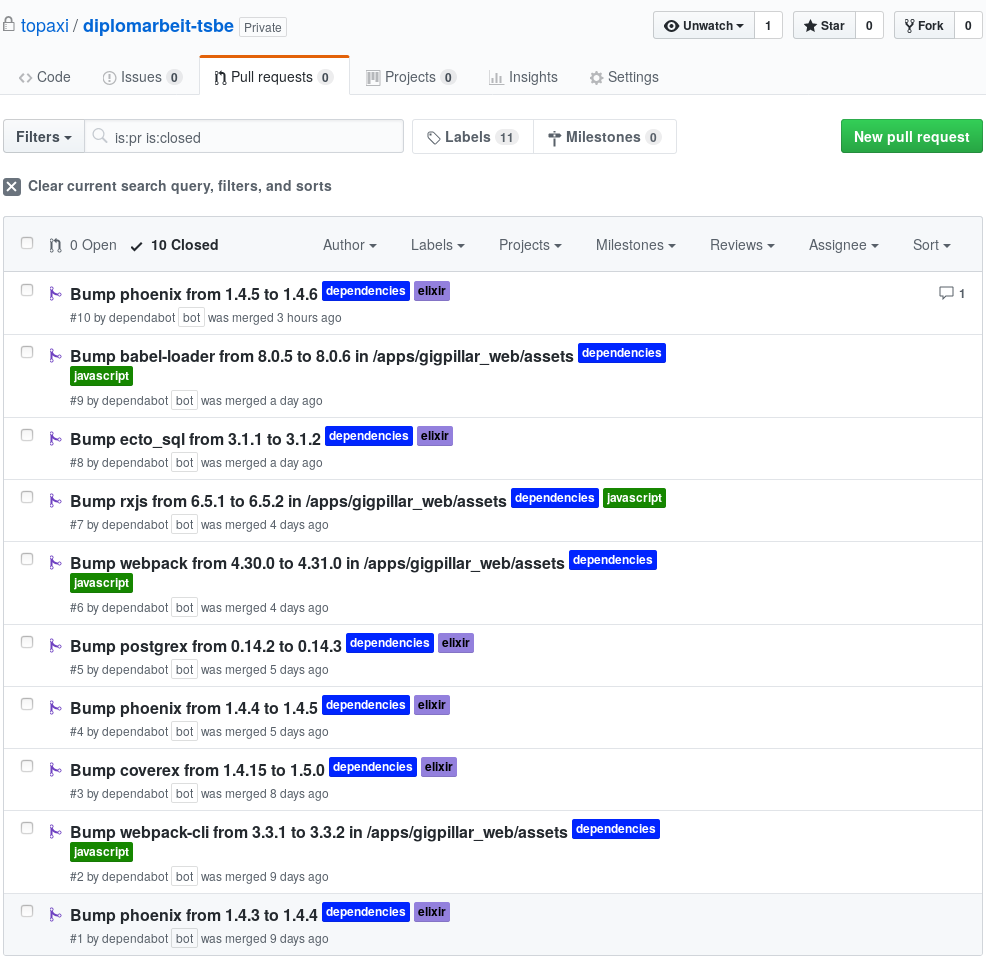
\includegraphics[width=1\textwidth]{realisierung/dependabot-updates-cropped.png}
  \caption{Dependabot: Pull-Requests für Updates}
\end{figure}

\clearpage
\section{Datenbankschema}\label{RealisierungsSchema}

Die folgenden Änderungen wurden am von der Konzeptphase vorgegebenen Schema
vorgenommen.

\subsubsection{Alle Entitäten}
Alle «created\_at» Felder wurden nach «inserted\_at» umbenannt, da dies die
Standardbenennung des Phoenix Frameworks ist.

\subsubsection{User}
Der Benutzer Entität wurde das Feld «password» nach «password\_hash» umbenannt,
damit klar ist, dass nicht ein Passwort sondern nur ein Hash abgespeichert wird.
Das Passwort wird mit \textbf{Argon2}\footnote{\url{https://en.wikipedia.org/wiki/Argon2}}
verschlüsselt und ist somit eine sichere Verschlüsselung.

\subsubsection{Genre}
Der Genre Entität sind im Konzept die Datumsfelder «update\_at» und «inserted\_at»
vergessen gegangen und wurden in der Realisierung nachgeführt.

\subsubsection{Gig}\label{RealisierungSchemaGig}
In der Gig Entität wurden drei weitere Felder hinzugefügt.
Die Felder «uuid» und «picture» dienen dazu, die beim Erfassen sowie
Bearbeiten eines Gigs hochgeladenen Bilder zu identifizieren.
Das zusätzliche Feld «tickets» ermöglicht es, beim Erfassen eines Gigs
einen Link zum Ticketvorverkauf zu hinterlegen.

\subsubsection{Location}
Die Location Entität erhielt bei der Realisierung zwei neue Felder,
«address» für die Adresse der Location und
«google\_place\_id» um die Referenz der Google API zu erhalten.

\clearpage
\subsection{Finales Schema}

\begin{figure}[!htb]
  \centering
  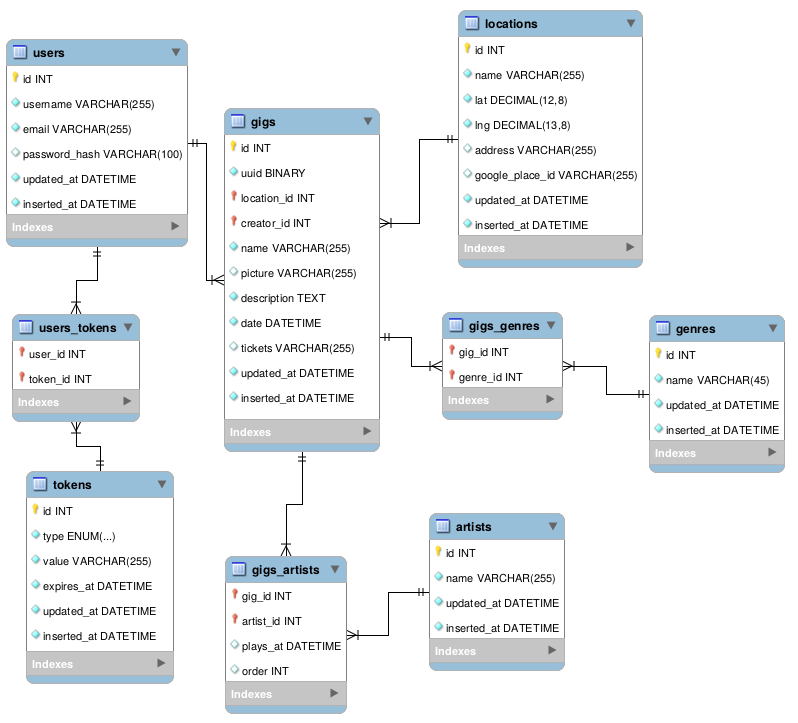
\includegraphics[width=0.95\textwidth]{realisierung/erd.png}
  \caption{Realisierung: Entity Relationship Diagram}
\end{figure}

\clearpage
\section{Berechtigungssystem}

Das Bearbeiten von Gigs wurde so eingeschränkt, dass nur angemeldete Benutzer Gigs erstellen dürfen und Benutzer nur eigene Gigs bearbeiten können.

Dazu wurde die Library «Canary»\footnote{\url{https://github.com/cpjk/canary}} verwendet. In der Datei «apps/gigpillar/lib/abilities.ex» wurden die Berechtigungen wie gefolgt umgesetzt:

\lstinputlisting[language=elixir,frame=single]{../apps/gigpillar/lib/abilities.ex}

\clearpage
\section{Location Autocomplete}

Das Location Autocomplete Feld wurde mit der «Google Place API»\footnote{\url{https://developers.google.com/places/web-service/autocomplete}} umgesetzt.

Die verwendete Library «google-api-elixir-client» implementiert die
Autocomplete API, jedoch fehlte noch die entsprechende Zusatzfunktion um
weitere Details, wie die geographischen Koordinaten, Adresse, etc., zu den gefundenen Locations abzufragen.

Die API um Details abzufragen wurden im Rahmen von diesem Projekt umgesetzt
und zurück an das originale Projekt beigesteuert.

Ausserdem musste eine Abhängigkeit auf den aktuellsten Stand gebracht werden.

Die beiden Beiträge für die Library sind auf Github zu finden:

\begin{itemize}
  \item{} \url{https://github.com/seanabrahams/google-api-elixir-client/pull/10/files}
  \item{} \url{https://github.com/seanabrahams/google-api-elixir-client/pull/11/files}
\end{itemize}

\clearpage
\section{HTML Erweiterungen}

Während der Entwicklung des Projektes, wurden einige spezielle HTML-Elemente
definiert. Diese Elemente wurden mit \textbf{LitElement}\footnote{\url{https://lit-element.polymer-project.org/}}
umgesetzt, und bieten gegenüber den Standard HTML-Elementen eigens definierte
Verhaltensweisen.

\subsubsection{<search-box>}

Das \textbf{<search-box>} Element wird für die Suche sowie diverse
Autocomplete-Elemente verwendet. Stylistisch sieht die Suchbox aus wie
ein normales Texteingabefeld, mit einer kleiner Lupe als Symbol.\\
\\
\noindent{}Beispiel:

\begin{lstlisting}[language=html,frame=single]
<search-box
  inputId="suche"
  src="/api/autocomplete"
  name="suche"
  placeholder="Suche..."
  value="Suchbegriff"
  debounce-time="300"></search-box>
\end{lstlisting}

\noindent{}Attribute:
\begin{itemize}
  \tightlist{}
  \item{} \textbf{inputId:} Das \textbf{id} Attribut für das Input Element innerhalb der Suchbox, z.B. im Zusammenhang mit einem \textbf{<label>} Element.
  \item{} \textbf{src:} URL für die Datenabfrage, bei Eingaben in das Textfeld wird jeweils eine \textbf{HTTP} Abfrage ausgelöst und ein \textbf{search-result} Ereignis ausgelöst.
  \item{} \textbf{name:} Der Name des Form-Elements.
  \item{} \textbf{placeholder:} Platzhaltertext welcher dargestellt wird wenn das Textfeld leer ist.
  \item{} \textbf{value:} Der Wert, welcher mit dem HTML-Formular mitgeschickt wird.
  \item{} \textbf{debounce-time:} Zeit in Millisekunden die mindestens vergehen muss, bevor eine neue Abfrage an den Server geschickt wird.
\end{itemize}

\subsubsection{<with-dropdown>}

Mit dem \textbf{<with-dropdown>} Element können Dropdowns realisiert werden.
Elemente mit dem Attribut \textbf{slot="dropdown"} werden initial nicht dargestellt.
Wird ein Element innerhalb des \textbf{<with-dropdown>} Element fokussiert, so werden die mit \textbf{slot="dropdown"} gekennzeichneten Elemente innerhalb eines Dropdown-Elements dargestellt.\\
\\
\noindent{}Beispiel:

\begin{lstlisting}[language=html,frame=single]
<with-dropdown>
  <input type="text">
  <ul slot="dropdown">
    <li>Lorem</li>
    <li>Ipsum</li>
  </ul>
</with-dropdown>
\end{lstlisting}

\subsubsection{<location-input>}

Das \textbf{<location-input>} Element wird verwendet um für einen Gig eine
Location auszuwählen. Es repräsentiert ein Suchfeld, das eine Abfrage über die
Google Place API macht. Wird eine Location ausgewählt, wird das Suchfeld durch
einen Text sowie Button ersetzt. Der Text beinhaltet den Namen der Location und
der Button ermöglicht es, die ausgewählte Location mit einer Neuen zu ersetzen.\\
\\
\noindent{}Beispiel:

\begin{lstlisting}[language=html,frame=single]
<location-input
  inputId="gig_location"
  name="gig[location]"
  location="{
    "name": "Dachstock",
    "google_place_id": "ChIJ-SskKr45jkcRPqmGB-ZGsRE"
  }"></location-input>
\end{lstlisting}

\noindent{}Attribute:
\begin{itemize}
  \tightlist{}
  \item{} \textbf{inputId:} Das \textbf{id} Attribut für das Input Element innerhalb des Location-Input, z.B. im Zusammenhang mit einem \textbf{<label>} Element.
  \item{} \textbf{name:} Der Name des Form-Elements.
  \item{} \textbf{location:} Ein \textbf{JSON}-Objekt einer Location, bestehend aus \textbf{name} und einer \textbf{id} oder \textbf{google\_place\_id}.
\end{itemize}

\subsubsection{<picture-input>}

Als verbessertes File-Input, wurde ein Ersatz für ein
\textbf{<input type=file>} Element geschrieben. Das \textbf{<picture-input>}
Element funktioniert als kompatibler Ersatz und bietet die selbe Funktionalität an.
Der Hauptunterschied liegt in der Darstellung, so wird beim \textbf{<picture-input>}
jederzeit eine Vorschau für das ausgewählte Bild dargestellt.\\
\\
\noindent{}Beispiel:

\begin{lstlisting}[language=html,frame=single]
<picture-input
  inputId="gig-picture"
  name="gig[picture]"
  value="http://example.com/my-picture.png"></picture-input>
\end{lstlisting}

\noindent{}Attribute:
\begin{itemize}
  \tightlist{}
  \item{} \textbf{inputId:} Das \textbf{id} Attribut für das Input Element innerhalb des Picture-Input, z.B. im Zusammenhang mit einem \textbf{<label>} Element.
  \item{} \textbf{name:} Der Name des Form-Elements.
  \item{} \textbf{value:} URL oder Datei des ausgewählten Bildes.
\end{itemize}

\clearpage
\subsubsection{<datetime-input>}

Das \textbf{<datetime-input>} Element kombiniert ein \textbf{<input type=date>}
mit einem \textbf{<input type=time>} zu einem Feld zusammen.
\\
\noindent{}Beispiel:

\begin{lstlisting}[language=html,frame=single]
<datetime-input
  inputId="datetime"
  dateLabel="Datum"
  timeLabel="Uhrzeit"
  name="datetime"
  value="2019-05-14T17:50:14.608Z"></datetime-input>
\end{lstlisting}

\noindent{}Attribute:
\begin{itemize}
  \tightlist{}
  \item{} \textbf{inputId:} Das \textbf{id} Attribut für das Input Element innerhalb des Datetime-Input, z.B. im Zusammenhang mit einem \textbf{<label>} Element.
  \item{} \textbf{dateLabel:} Beschriftung für das Datumsfeld.
  \item{} \textbf{timeLabel:} Beschriftung für das Zeitfeld.
  \item{} \textbf{name:} Der Name des Form-Elements.
  \item{} \textbf{value:} Datum mit Zeit im \textbf{ISO 8601}\footnote{\url{https://de.wikipedia.org/wiki/ISO_8601}} Format.
\end{itemize}

\subsubsection{<artists-input>}

Das \textbf{<artists-input>} ist ein spezifisches Feld für das Erfassen von
Künstlern für ein Konzert. Es Sucht über den Server bereits existierende
Künstler, und bietet diese zur Auswahl an. Zusätzlich kann für jeden
ausgewählten Künstler eine Zeit angegeben werden, an welcher deren Auftritt
stattfindet.\\
\\
\noindent{}Beispiel:

\begin{lstlisting}[language=html,frame=single]
<artists-input
  inputId="artists"
  name="gig[artists]"
  placeholder="K&uuml;nstler suchen..."
  value="[
    {"id":42,"name":"Parkway Drive","plays_at":"23:00"},
    {"id":23,"name":"The Ghost Inside","plays_at":"21:00"}
  ]"></artists-input>
\end{lstlisting}

\noindent{}Attribute:
\begin{itemize}
  \tightlist{}
  \item{} \textbf{inputId:} Das \textbf{id} Attribut für das Input Element innerhalb des Artists-Input, z.B. im Zusammenhang mit einem \textbf{<label>} Element.
  \item{} \textbf{name:} Der Name des Form-Elements.
  \item{} \textbf{placeholder:} Platzhalter für das Suchfeld.
  \item{} \textbf{value:} Eine Liste von \textbf{JSON}-Objekten der einem Gig assozierten Künstler.
\end{itemize}

\clearpage
\section{Asset Optimierungen}

Für die Produktionsumgebung, wurden diverse Optimierungen vorgenommen:

\begin{itemize}
  \tightlist{}
  \item{} Terser Plugin um JavaScript Code zu optimieren.
  \item{} Plugin um Funktionen zu deduplizieren.
  \item{} HTML Minifier Plugin um HTML innerhalb von JavaScript zu optimieren.
  \item{} Imagemin Plugin um Bilder auf Dateigrösse zu optimieren.
  \item{} CSS Optimierungsplugin
  \item{} Zopfli Kompression
  \item{} Brotli Kompression
\end{itemize}

Diese Plugins reduzieren die Dateigrössen von JavaScript, CSS sowie Bilddateien.
Die reduzierte Grösse kommt Benutzern mit schlechteren Internetverbindungen, wie z.B. im mobilen Netz, entgegen.

\begin{longtable}[]{@{}llr@{}}
  \toprule
  \textbf{Optimierungen}        & \textbf{Datei} & \textbf{Grösse}\tabularnewline
  \midrule
  Keine                         & app.js         & 1000 KiB\tabularnewline
  Produktionsmodus              & app.js         & 397 KiB\tabularnewline
  ” und Terser Plugin           & app.js         & 125 KiB\tabularnewline
  ” und Funktionsdeduplizierung & app.js         & 123 KiB\tabularnewline
  ” und HTML Minifier           & app.js         & 122 KiB\tabularnewline
  ” mit Zopfli                  & app.js.gz      & 25.2 KiB\tabularnewline
  ” mit Brotli                  & app.js.br      & 23.0 KiB\tabularnewline
  \bottomrule
  \caption{JavaScript Optimierungen}
\end{longtable}

\begin{longtable}[]{@{}llr@{}}
  \toprule
  \textbf{Optimierungen}       & \textbf{Datei} & \textbf{Grösse}\tabularnewline
  \midrule
  Keine                        & app.css        & 10.5 KiB\tabularnewline
  Produktionsmodus             & app.css        & 10.5 KiB\tabularnewline
  ” und CSS Optimierungsplugin & app.css        & 8.58 KiB\tabularnewline
  \bottomrule
  \caption{CSS Optimierungen}
\end{longtable}

\begin{longtable}[]{@{}llr@{}}
  \toprule
  \textbf{Optimierungen}       & \textbf{Datei}   & \textbf{Grösse}\tabularnewline
  \midrule
  Keine                        & background-1.jpg & 1.79 MiB\tabularnewline
  Produktionsmodus             & background-1.jpg & 1.79 MiB\tabularnewline
  ” und Imagemin (Qualität 75) & background-1.jpg & 278 KiB\tabularnewline
  \bottomrule
  \caption{Bilder Optimierungen}
\end{longtable}

\clearpage
\section{File Upload}

Für den Upload der Bilder von Gigs, wird die Software \textbf{"<minio">}\footnote{\url{https://min.io/}} eingesetzt.
Die Software ist mit der \textbf{Amazon Simple Storage Service} (kurz \textbf{Amazon S3}) kompatibel, und bietet sich daher
stark an da es bereits viele Libraries gibt, die den Upload erleichtern.

Für die Anbindung an \textbf{minio} werden die Libraries \textbf{ArcEcto}, \textbf{Arc} und \textbf{ExAws} eingesetzt.

Da die Bilder während dem Erstellen eines Gigs bereits hochgeladen werden, existiert für die Gigs
noch kein \textbf{id} Feld, dass von der Datenbank automatisch generiert wird.
Um die Bilder dennoch referenzieren zu können, wurde im Datenbankschema ein
Feld \textbf{"<uuid">} eingefügt (siehe \ref{RealisierungSchemaGig}).
Das \textbf{uuid} Feld wird mit einem möglichst einzigartigen Wert abgefüllt,
der Wert entspricht dem \textbf{UUID version 4}\footnote{\url{https://de.wikipedia.org/wiki/Universally_Unique_Identifier}} Standard.

Die \textbf{Arc} Library bietet eine einfache API an, um die hochgeladenen Bilder
auf die von der Webapplikation verwendeten Grössen zuzuschneiden. Dazu wird auf dem
Server die Software \textbf{"<ImageMagick">}\footnote{\url{https://imagemagick.org/}}
benötigt.

Es werden für jedes hochgeladene Bild zwei Grössen generiert,
\textbf{288$\times$224} Pixel für in Auflistungen und \textbf{160$\times$56}
Pixel für Suchresultate sowie im Bearbeitungsformular.\\

\noindent{}So werden bei einem Upload folgende Bilder abgelegt:
\begin{itemize}
  \tightlist{}
  \item{} gigs/\{uuid\}/original.ext
  \item{} gigs/\{uuid\}/list.ext
  \item{} gigs/\{uuid\}/thumbnail.ext
\end{itemize}

\section{OpenStreetMap}

Auf der Gig Detailansicht, wird eine OpenStreetMap eingebunden. Damit
die OpenStreetMap Karte korrekt dargestellt wird, mussten die Geokoordinaten
auf einzelne sogennante "<Tiles"> berechnet werden. Ein Tile ist ein einzelnes
\textbf{256$\times$256} Pixel Teilbild der Weltkarte, die Tiles unterscheiden
sich je nach Zoomlevel und muss entsprechend ausgerechnet werden.

Die genauere Beschreibung der Funktionsweise ist auf dem
\href{https://wiki.openstreetmap.org/wiki/Slippy\_map\_tilenames}{OpenStreetMap Wiki}
Dokumentiert\footnote{\url{https://wiki.openstreetmap.org/wiki/Slippy\_map\_tilenames}}.

Für die Programmiersprache Elixir ist auf dem Wiki kein Beispiel vorhanden und musste
entsprechend adaptiert werden.

\clearpage
\section{SEO - Microdata}

Auf der Gig Detailansicht wird für Suchmaschinen ein zusätzliches Element mit
\href{https://json-ld.org/}{JSON-LD} ausgegeben. Dieses Element ist für die
normalen Besucher nicht sichtbar.\\

\noindent{}Beispiel:

\lstinputlisting[language=html,frame=single]{realisierung/jsonld-example.html}

\clearpage
Während der Umsetzung ist durch das Validierungs-Tool\footnote{\url{https://search.google.com/structured-data/testing-tool}}
von Google aufgefallen, dass diverse empfohlene Felder nicht vorhanden sind.
Diese Felder sind optional und sind vom umgesetzten Datenmodell noch nicht abgedeckt.

\begin{figure}[!htb]
  \centering
  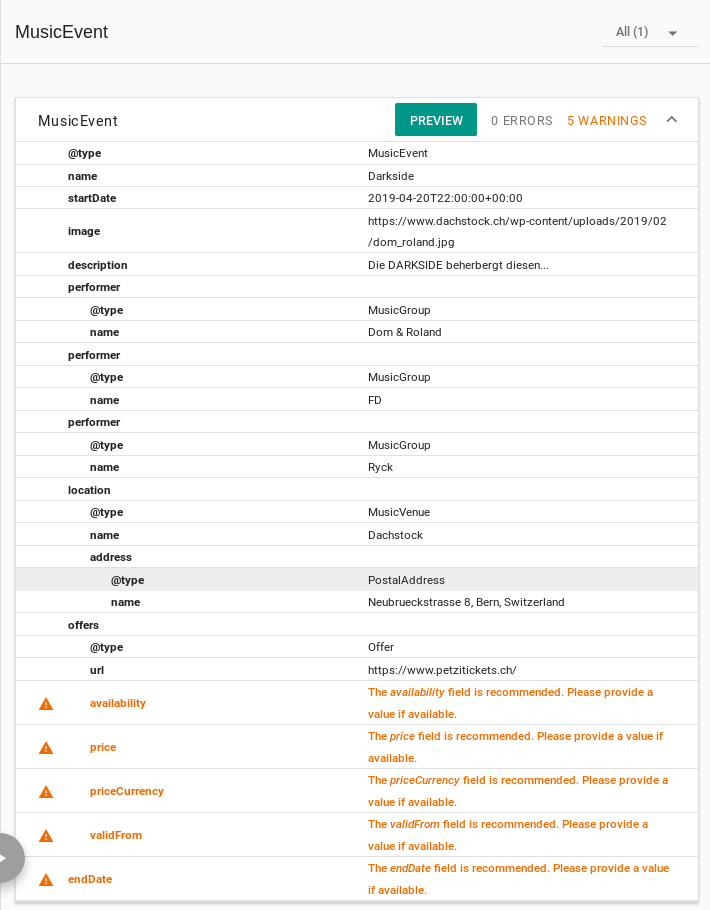
\includegraphics[width=0.95\textwidth]{realisierung/json-ld-validation.png}
  \caption{JSON-LD: Validierung}
\end{figure}

\clearpage
\section{Suche}

Die Suche wurde mit einem "<einfachen"> SQL umgesetzt, der eingegebene
Suchtext wird nach Wörter aufgeteilt und in den entsprechenden Datenbankfeldern
gesucht.
Das Suchresultat kann ausserdem mit den Parametern \textbf{from},
\textbf{to} und \textbf{genre} weiter eingeschränkt werden.\\
\\
\noindent{}Nachfolgend, die implementierte SQL Abfrage in Elixir:

\lstinputlisting[language=elixir,frame=single,firstline=132,lastline=169]{../apps/gigpillar/lib/gigpillar/gigs.ex}

\clearpage
\section{Probleme}\label{AppendixRealisierungProbleme}

\subsection{Dependency Konflikt}

\subsubsection{ExAws}

Die Library \textbf{ExAws} hat nach der Installation folgenden Fehler ausgelöst:

\begin{lstlisting}[frame=single]
Failed to use "poison" (version 4.0.1) because
  arc (version 0.11.0) requires ~> 2.2 or ~> 3.1
  coverex (version 1.5.0)
    requires ~> 3.0 or ~> 3.1 or ~> 4.0
  deps/google_api_client/mix.exs
    requires ~> 1.5 or ~> 2.0 or ~> 3.0 or ~> 4.0
  wallaby (version 0.22.0) requires >= 1.4.0
  mix.lock specifies 4.0.1

** (Mix) Hex dependency resolution failed, relax the version
  requirements of your dependencies or unlock them (by using
  mix deps.update or mix deps.unlock). If you are unable to
  resolve the conflicts you can try overriding with
  {:dependency, "~> 1.0", override: true}
\end{lstlisting}

Erste Versuche, die Abhängigkeit in der Gigpillar oder GigpillarWeb Applikation
zu überschreiben ist gescheitert.
Dieses Problem konnte behoben werden, in dem im \textbf{mix.exs} der Umbrella
Applikation die \textbf{poison} Abhängigkeit mit der \textbf{override} Option
eingefügt wurde.

\begin{lstlisting}[language=elixir,frame=single]
defmodule Gigpillar.Umbrella.MixProject do
  defp deps do
    [
      {:poison, "~> 4.0", runtime: false, override: true}
    ]
  end
end
\end{lstlisting}

\clearpage
\subsection{Formularbehandlung in Phoenix}

Da ich das Phoenix Framework bisher nur für \textbf{REST} APIs verwendet habe,
hatte ich einige Probleme mit den vom Framework zur Verfügung gestelten
Formularfunktionen.
Dies hat mir viel mehr Zeit beansprucht als initial angenommen.

In den meisten Tutorials, wurde die API mit einer \textbf{form\_for} Funktion
vorgestellt, diese Funktioniert jeweils nur im Zusammenhang mit einem
Ecto-Changeset\footnote{\url{https://hexdocs.pm/ecto/Ecto.Changeset.html}}.
Jedoch wird beim Login sowie der Suche kein solches Changeset verwendet.

Nach ausgiebigem durchlesen der offiziellen Dokumentation vom Phoenix Framework,
fand ich schlussendlich eine
\textbf{form\_tag}\footnote{\url{https://hexdocs.pm/phoenix\_html/Phoenix.HTML.Tag.html\#form\_tag/2}}
Funktion die auch ohne Changeset funktioniert.

Einige Zeit später fand ich jedoch im Phoenix Source Code\footnote{\url{https://github.com/phoenixframework/phoenix\_html/blob/f9a4f38/lib/phoenix\_html/form_data.ex\#L51}}
heraus, dass für das von Phoenix bereitgestellte Verbindungsobjekt
\textbf{Plug.Conn} das \textbf{Phoenix.HTML.FormData} Protokol implementiert
wird.

Das Verwenden des \textbf{Plug.Conn} Objektes erleichtert die Benützung der
Formular Funktionen um einiges, da entsprechende Form Aktionen nicht mehr
explizit definiert werden müssen. Zudem wird das zuordnen der Daten ins
HTML automatisch vom Framework übernommen, was diverse Fehlerquellen
eliminiert.

\subsection{Datumsbehandlung}

Die Datum und Zeitanzeigen in der Applikation wurden mit der Zeit immer wie
komplizierter. Insbesondere wenn Zeitzonen involviert sind, war es kaum mehr
übersichtlich wann welche Daten vorhanden sind. Um nicht mehr zwischen den
verschiedenen Datenstrukturen von Elixir zu unterscheiden müssen, wurde die
Library \textbf{"<Timex">}\footnote{\url{https://github.com/bitwalker/timex}}
installiert.

Timex bietet diverse Funktionen um jegliche Datum/Zeit bezogenen Datenstrukturen
zu manipulieren und formatieren.

\subsection{Behandlung von Datenrelationen}

TODO...

\clearpage
\section{Tests}\label{RealisierungsTests}

Die Tests können über das Kommando \textbf{mix test} ausgeführt werden.

\noindent{}Beispiel:

\begin{figure}[!htb]
  \centering
  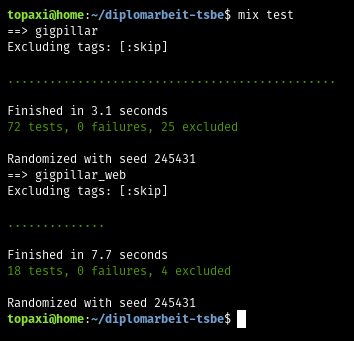
\includegraphics[width=0.75\textwidth]{realisierung/test-run.png}
  \caption{Tests: Ausführung der automatisierten Tests}
\end{figure}

\noindent{}Einige Tests werden derzeit noch übersprungen, da nicht genug Zeit vorhanden
war.

Damit die Browsertests funktionieren, muss auf dem Zielsystem der
\textbf{Chromedriver} installiert werden. Chromedriver kann entweder von der
offiziellen Webseite\footnote{\url{http://chromedriver.chromium.org/}}
heruntergeladen oder über den Node Package Manager (NPM) installiert werden.\\
\\
Installation mit NPM:

\begin{lstlisting}[language=bash,frame=single]
$ npm install -g chromedriver
\end{lstlisting}


\clearpage
\section{Testprotokoll}\label{RealisierungsTestprotokoll}

\setcounter{acceptancetest}{0}

\acceptancetest[Damian Senn][16.05.2019][OK]
{Es ist möglich nach Konzerten in einem bestimmten Ort zu suchen.}
{Nach auswählen von «Berlin» in der Suche, werden nur noch Konzerte in Berlin aufgelistet.}

\acceptancetest[Damian Senn][16.05.2019][OK]
{Es ist möglich eine Suche weiter nach Genre einzuschränken.}
{Nach auswählen von «Rock» in einem Suchresultat, werden nur noch Rock-Konzerte aufgelistet.}

\clearpage

\acceptancetest[Damian Senn][16.05.2019][OK]
{Responsive - Homepage}
{Sieht auf Desktop, Tablet und Mobile gut aus und stellt jeweils alle relevanten Daten dar.}

\acceptancetest[Damian Senn][16.05.2019][OK]
{Browserkompatibilität - Homepage}
{Funktioniert in den unterstützten Browsern.}

\clearpage

\acceptancetest[Damian Senn][16.05.2019][OK]
{Responsive - Suche}
{Sieht auf Desktop, Tablet und Mobile gut aus und stellt jeweils alle relevanten Daten dar.}

\acceptancetest[Damian Senn][16.05.2019][OK]
{Browserkompatibilität - Suche}
{Funktioniert in den unterstützten Browsern.}

\clearpage

\acceptancetest[Damian Senn][16.05.2019][OK]
{Responsive - Gig Ansicht}
{Sieht auf Desktop, Tablet und Mobile gut aus und stellt jeweils alle relevanten Daten dar.}

\acceptancetest[Damian Senn][16.05.2019][OK]
{Browserkompatibilität - Gig Ansicht}
{Funktioniert in den unterstützten Browsern.}

\clearpage

\acceptancetest[Damian Senn][16.05.2019][OK]
{Responsive - Login}
{Sieht auf Desktop, Tablet und Mobile gut aus und stellt jeweils alle relevanten Daten dar.}

\acceptancetest[Damian Senn][16.05.2019][OK]
{Browserkompatibilität - Login}
{Funktioniert in den unterstützten Browsern.}

\clearpage

\acceptancetest[Damian Senn][16.05.2019][OK]
{Responsive - Registrierung}
{Sieht auf Desktop, Tablet und Mobile gut aus und stellt jeweils alle relevanten Daten dar.}

\acceptancetest[Damian Senn][16.05.2019][OK]
{Browserkompatibilität - Registrierung}
{Funktioniert in den unterstützten Browsern.}

\clearpage

\acceptancetest[Damian Senn][16.05.2019][OK]
{Responsive - Gig erfassen}
{Sieht auf Desktop, Tablet und Mobile gut aus und stellt jeweils alle relevanten Daten dar.}

\acceptancetest[Damian Senn][16.05.2019][OK]
{Browserkompatibilität - Gig erfassen}
{Funktioniert in den unterstützten Browsern.}

\clearpage

\acceptancetest[Damian Senn][16.05.2019][OK]
{Gig erfassen}
{Folgende Daten können erfasst werden:
  \begin{itemize}
    \tightlist{}
    \item{} Name
    \item{} Bild \textit{(optional)}
    \item{} Location
    \item{} Datum
    \item{} Zeit \textit{(optional)}
    \item{} Künstler mit optionaler Start-Zeit
    \item{} Beschreibung
    \item{} Link zum Ticketvertreiber \textit{(optional)}
  \end{itemize}}

\acceptancetest[Damian Senn][16.05.2019][OK]
{Neue Gigs tauchen in der Suche auf.}
{Der neu erstellte Gig taucht in der Suche auf.}

\clearpage

\acceptancetest[Damian Senn][16.05.2019][Fehlerhaft]
[Die Benutzerprofil Funktionalität fehlt komplett.]
{Responsive - Benutzerprofil}
{Sieht auf Desktop, Tablet und Mobile gut aus und stellt jeweils alle relevanten Daten dar.}

\acceptancetest[Damian Senn][16.05.2019][Fehlerhaft]
[Die Benutzerprofil Funktionalität fehlt komplett.]
{Browserkompatibilität - Benutzerprofil}
{Funktioniert in den unterstützten Browsern.}

\clearpage

\acceptancetest[Damian Senn][16.05.2019][Fehlerhaft]
[Es gibt keine Möglichkeit ein vergessenes Passwort zurückzusetzem.]
{Responsive - Passwort-Reset}
{Sieht auf Desktop, Tablet und Mobile gut aus und stellt jeweils alle relevanten Daten dar.}

\acceptancetest[Damian Senn][16.05.2019][Fehlerhaft]
[Es gibt keine Möglichkeit ein vergessenes Passwort zurückzusetzem.]
{Browserkompatibilität - Passwort-Reset}
{Funktioniert in den unterstützten Browsern.}

\clearpage

\acceptancetest[Damian Senn][16.05.2019][OK]
{Security - Suche}
{Das Suchfeld ist resistent gegen XSS und SQL-Injection}

\acceptancetest[Damian Senn][16.05.2019][OK]
{Security - Login}
{Das Login ist resistent gegen XSS und SQL-Injection}

\clearpage

\acceptancetest[Damian Senn][16.05.2019][Fehlerhaft]
[Die Benutzerprofil Funktionalität fehlt komplett.]
{Security - Benutzerprofil}
{Das Benutzerprofil ist resistent gegen XSS und SQL-Injection}

\acceptancetest[Damian Senn][16.05.2019][OK]
{Security - Gig erfassen}
{Das Gig erfassen Formular ist resistent gegen XSS und SQL-Injection}

\clearpage
\section{Offene Punkte}

Einige Kriterien konnten bisher noch nicht umgesetzt werden, dies ist vor allem
auf die bereits erläuterten Probleme~(\ref{AppendixRealisierungProbleme})
zurückzuführen.

\subsection{Genre Zuordnung für Gigs}

Während die Filterung nach Genre bereits funktioniert, ist es noch nicht
möglich, einem Gig ein oder mehrere Genres zuzuweisen.

Der Aufwand dies nachzuliefern wird auf circa 8 bis 10 Stunden geschätzt.

\subsection{Benutzer Profil}

Das Benutzerprofil, in welchem angemeldete Besucher ihre Daten wie E-Mail,
Benutzername, Passwort, etc. bearbeiten können, wurde noch nicht umgesetzt.
Da das Benutzerprofil nicht ein zentraler Bestandteil der Applikation ist,
habe ich mich dazu entschieden, die Umsetzung zu verschieben.

\subsection{Passwort-Reset Funktionalität}

Benutzer die ihr Passwort vergessen haben, haben derzeit keine Möglichkeit
dieses zurückzusetzen. Da die Applikation ohne diese Funktion ihre
Grundfunktionalität erfüllen kann, wurde dieses Feature noch nicht umgesetzt.

\subsection{Screenshot Tests}

Wie bereits in der Studie~(\ref{WallabyPercy}) identifiziert, ist das
Wallaby Test-Framework leider nicht mit \href{https://percy.io/}{percy.io}
kompatibel, es ist denkbar eine Integration selber umzusetzen. Da die
Umsetzung der Screenshot Tests keine direkter Nutzen für die Applikation
bietet, wurde dies noch nicht umgesetzt.

\subsection{Expliziter Ort Kontext}

Implizit ist in den Konzept Mockups zu erkennen, dass auf der Startseite sowie
in der Suche automatisch nach der Stadt, in welcher sich der Besucher befindet,
gefiltert wird. Dies wurde im Software-Konzept weiter ausgearbeitet und es wurde
definiert, dass die Stadt des Besuchers über eine GeoIP Datenbank zugeordnet wird.
Diese Zuordnung von Besucher IP nach Stadt wurde umgesetzt, jedoch werden die
Inhalte der Webseite noch nicht implizit danach gefiltert.

Das Kriterium, dass die Suche nach Ort einschränken soll, ist jedoch durch den
Suchfilter abgedeckt.

\clearpage
\subsection{Mögliche Erweiterungen}

Durch die geographischen Koordinaten die wir durch die Google Places API erhalten,
ist es denkbar, einen weiteren Suchfilter zu implementieren, der über einen Radius
arbeitet. Als Beispiel könnte so nach Konzerten in der Nähe von Bern mit einem
Radius von 30 Kilometern gesucht werden.

Dazu habe ich bereits eine Lösung im Internet\footnote{\url{https://www.movable-type.co.uk/scripts/latlong-db.html}}
gefunden, die relativ einfach zu implementieren wäre.

\section{Installationsanleitung}\label{installation}

\subsection{Benötigte Software}

\subsubsection{Server}

Auf dem Server wo die Applikation betrieben werden soll müssen die folgenden
Software Pakete installiert werden:

\begin{itemize}
  \tightlist{}
  \item{} Erlang OTP Version 22.0
  \item{} rebar Version 3.10.0
  \item{} Elixir Version 1.8.0
  \item{} Imagemagick 6.9
\end{itemize}

Alternativ kann zu einem offiziellen Docker Image\footnote{\url{https://hub.docker.com/\_/elixir/}}
gegriffen werden, dieses stellt bereits alle nötigen Software Pakete zur
Verfügung.

Bei der Installation des Servers oder Images, muss ausserdem die GeoIP
Datenbank installiert werden, diese kann unter der folgenden URL
heruntergeladen werden:

\url{https://geolite.maxmind.com/download/geoip/database/GeoLite2-City.tar.gz}

Damit die Server Applikation die Datenbank findet, muss die System Environment
Variable \textbf{GEOIP\_DATABASE\_FILE} gesetzt werden.

\subsubsection{Testumgebung}

Die Testumgebung hat die selben Anforderungen wie der Server.

Damit die Browsertests funktionieren, muss auf dem Zielsystem der
\textbf{Chromedriver} installiert werden. Chromedriver kann entweder von der
offiziellen Webseite\footnote{\url{http://chromedriver.chromium.org/}}
heruntergeladen oder über den Node Package Manager (NPM) installiert werden.\\
\\
Installation mit NPM:

\begin{lstlisting}[language=bash,frame=single]
$ npm install -g chromedriver
\end{lstlisting}


\clearpage
\subsection{Benötigte Dienste}

Für den Betrieb der Server Applikation sowie der Testumgebung werden
zusätzliche Dienste wie die Datenbank oder Dateiserver benötigt.\\
\\
Für die Umsetzung wurde die von Phoenix als Standard definierte
Datenbanksoftware \textbf{PostgreSQL}\footnote{\url{https://www.postgresql.org/}} verwendet.\\
\\
Für das Sessionmanagement von Besuchern wird der Key-Value Store \textbf{redis}
verwendet. Es ist denkbar, das Redis in Zukunft auch für Caching von Resourcen
verwendet werden kann.\\
\\
File-Uploads, vor allem für Bilder, wird mit der \textbf{minio} Software
verwaltet.\\
\\
\noindent{}Folgende Dienste sind nötig für den Betrieb der Applikation:

\begin{itemize}
  \tightlist{}
  \item{} PostgreSQL Version 11
  \item{} Redis 5
  \item{} minio (RELEASE.2019-05-02T19-07-09Z)
\end{itemize}

\clearpage
\subsection{Umgebungsvariablen}

\begin{longtable}[]{@{}lp{7cm}@{}}
  \toprule
  \textbf{Name}                     & \textbf{Beschreibung}\tabularnewline
  \midrule
  AWS\_S3\_BUCKET                   & Amazon S3 oder minio Bucket Name\tabularnewline
  AWS\_ACCESS\_KEY\_ID              & Amazon oder minio Access Key\tabularnewline
  AWS\_SECRET\_ACCESS\_KEY          & Amazon oder minio Secret Acces Key\tabularnewline
  AWS\_REGION                       & Amazon Region ("<local"> für minio)\tabularnewline
  AWS\_S3\_SCHEME                   & Amazon URL Schema ("<https"> oder "<http">)\tabularnewline
  AWS\_S3\_HOST                     & Amazon S3 oder minio Hostname\tabularnewline
  AWS\_S3\_PORT                     & Amazon S3 oder minio Port\tabularnewline
  GIGPILLAR\_WEB\_HOST              & Hostname der Applikation, z.B. "<gigpillar.com">\tabularnewline
  GIGPILLAR\_WEB\_SECRET\_KEY\_BASE & Ein zufällig generierter Wert, wird für die Verschlüsselung der Sessiondaten benötigt.\tabularnewline
  GIGPILLAR\_WEB\_DEFAULT\_CITY     & Stadt die angezeigt werden soll, wenn für den Besucher keine zugeordnet werden kann.\tabularnewline
  GIGPILLAR\_ASSET\_HOST            & Basis URL für den File-Upload Server, z.B. "<http://localhost:4040">\tabularnewline
  POSTGRES\_USER                    & Der Datenbank Benutzername\tabularnewline
  POSTGRES\_PASSWORD                & Das Datenbank Benutzer Passwort\tabularnewline
  POSTGRES\_DB                      & Der Datenbank Name\tabularnewline
  POSTGRES\_HOSTNAME                & Der Hostname des Datenbank Servers\tabularnewline
  POSTGRES\_POOL\_SIZE              & Die Anzahl Verbindungen die zur Datenbank gemacht werden sollen.\tabularnewline
  GEOIP\_DATABASE\_FILE             & Pfad zum GeoIP Datenbank Archiv.\tabularnewline
  GOOGLE\_API\_KEY                  & Der Google API Schlüssel.\footnote{\url{https://developers.google.com/places/web-service/get-api-key}}\tabularnewline
  REDIS\_HOST                       & Der redis Hostname \tabularnewline
  REDIS\_PORT                       & Der redis Port\tabularnewline
  \bottomrule
  \caption{Betrieb: Umgebungsvariablen}
\end{longtable}

\clearpage
\subsection{Initialen Benutzer erstellen}

Es wurde ein Skript erstellt um den ersten, initialen Benutzer zu erstellen.
Dies sollte vorallem für Testzwecke verwendet werden und nicht auf der
produktiven Umgebung.

\begin{lstlisting}[language=bash,frame=single]
$ mix gigpillar.create_user
\end{lstlisting}

\noindent{}Beispiel einer erfolgreichen Durchführung des Skripts:

\begin{figure}[!htb]
  \centering
  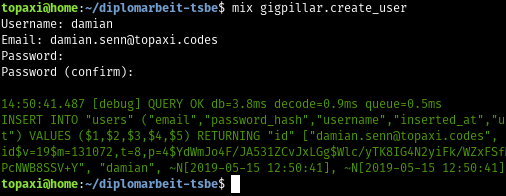
\includegraphics[width=0.9\textwidth]{einfuehrung/create-user.png}
  \caption{Initialen Benutzer erstellen}
\end{figure}

\clearpage
\subsection{Grundsetup und Start}

Zuerst muss ein Secret erstellt werden, dieses wird für die Verschlüsselung der
Besucher Session Daten verwendet, dies muss generiert und sicher aufbewahrt
werden. Wird das Secret ausgewechselt, werden alle Benutzer die eingeloggt sind
automatisch ausgeloggt. Das Secret darf daher \textbf{nur} ausgewechselt
werden, falls dieses aus Versehen in die Öffentlichkeit gelangt!

\begin{lstlisting}[language=bash,frame=single]
$ mix phx.gen.secret
wcR6neHuJjwErwFAbZPLUPGj5yo3ciue4dLRNz6EwQIGYhL0T5PexUfyx/zC
\end{lstlisting}

\noindent{}Unter \textbf{keinen} Umständen soll das obige Secret verwendet werden!
\textbf{Es muss ein neues Secret für den Betrieb generiert werden!}

\begin{lstlisting}[language=bash,frame=single]
$ export GIGPILLAR_SECRET_KEY_BASE=wcR6neHuwFAbZLUPGj5yiue4d
\end{lstlisting}

\noindent{}Nach dem Erstellen des Secrets müssen die Abhängigkeiten instaliert und
kompiliert werden.\\
\\
\noindent{}Herunterladen und kompilieren der Elixir Abhängigkeiten:

\begin{lstlisting}[language=bash,frame=single]
$ mix deps.get --only prod
$ MIX_ENV=prod mix compile
\end{lstlisting}

\noindent{}Herunterladen und kompilieren der JavaScript Abhängigkeiten:

\begin{lstlisting}[language=bash,frame=single]
$ cd apps/gigpillar_web/assets
$ yarn --frozen-lockfile
$ npx webpack --mode production
$ cd -
$ mix phx.digest
\end{lstlisting}

\noindent{}Die Applikation ist nun bereit für den Start im Produktionsmodus,
dazu muss nun nur noch das \textbf{MIX\_ENV} sowie der \textbf{Port} definiert
werden:

\begin{lstlisting}[language=bash,frame=single]
$ MIX_ENV=prod PORT=4004 mix phx.server
\end{lstlisting}

\chapter{Einführung}\label{AppendixEinführung}

\section{Installationsanleitung}

\subsection{Benötigte Software}

\subsubsection{Server}
- geoip db
- imagemagick

\subsubsection{Testumgebung}
- webdriver (npm, für tests)

\subsection{Umgebungsvariablen}

\begin{longtable}[]{@{}ll@{}}
  \toprule
  \textbf{Name}            & \textbf{Beschreibung}\tabularnewline
  \midrule
  AWS\_S3\_BUCKET          & \tabularnewline
  AWS\_ACCESS\_KEY\_ID     & \tabularnewline
  AWS\_SECRET\_ACCESS\_KEY & \tabularnewline
  AWS\_REGION              & \tabularnewline
  AWS\_S3\_SCHEME          & \tabularnewline
  AWS\_S3\_HOST            & \tabularnewline
  AWS\_S3\_PORT            & \tabularnewline
  GIGPILLAR\_ASSET\_HOST   & \tabularnewline
  POSTGRES\_USER           & \tabularnewline
  POSTGRES\_PASSWORD       & \tabularnewline
  POSTGRES\_DB             & \tabularnewline
  POSTGRES\_HOSTNAME       & \tabularnewline
  POSTGRES\_POOL\_SIZE     & \tabularnewline
  \bottomrule
\end{longtable}

\chapter{Schlussbetrachtung}

\label{ReportSchlussbetrachtung}



%------------------------------------------------------------------------------
% APPENDICES
%------------------------------------------------------------------------------

\appendix % Cue to tell LaTeX that the following "chapters" are Appendices

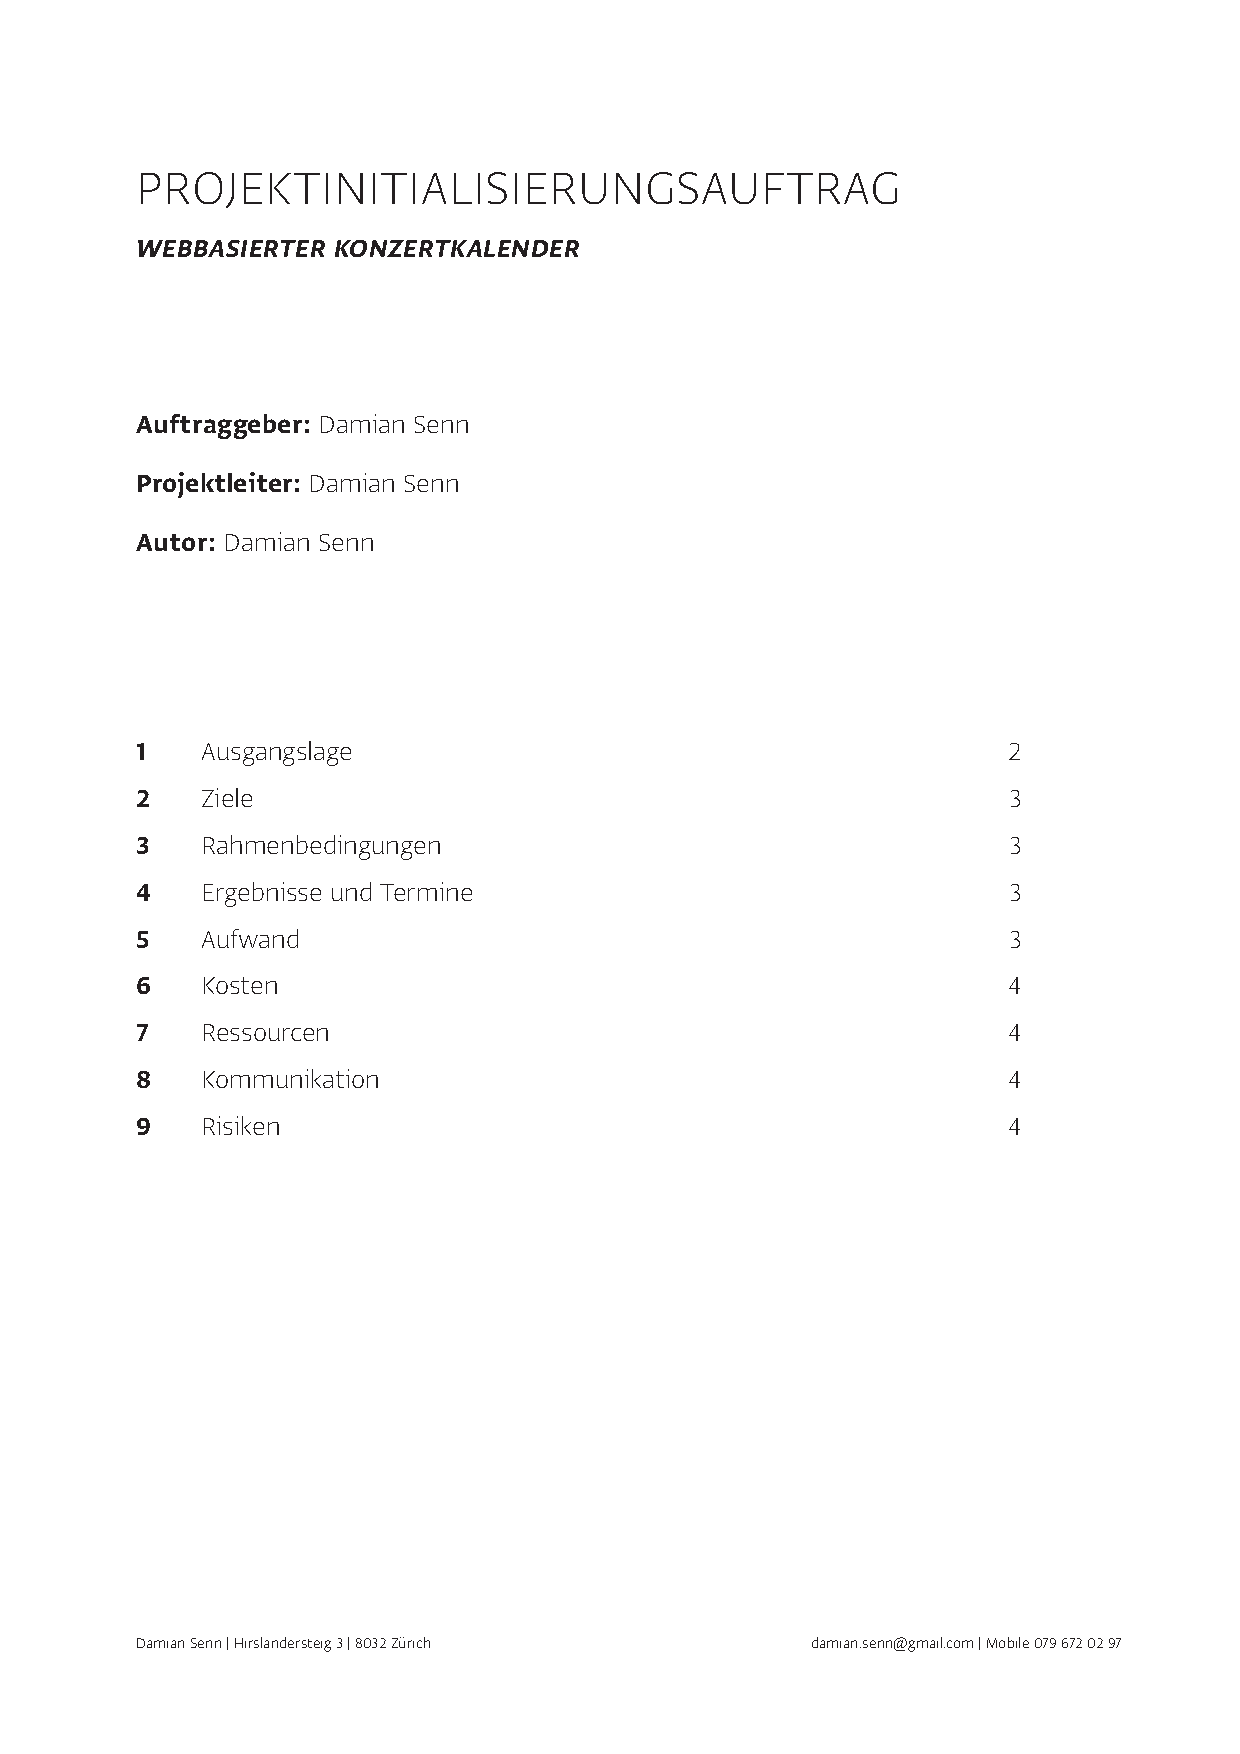
\includepdf[pages=1,pagecommand={\thispagestyle{empty}\Hide\chapter{Projektinitialisierungsauftrag}}]{eingabe/Projektinitialisierungsauftrag.pdf}
\includepdf[pages=2-,pagecommand={\thispagestyle{empty}}]{eingabe/Projektinitialisierungsauftrag.pdf}

\chapter{Projektauftrag}

\label{AppendixProjektauftrag}

\section{Zweck des Dokuments}\label{ProjektauftragZweck}

Der Projektauftrag ist die verbindliche Vereinbarung zwischen Auftraggeber und
Projektleiter, und bildet die Grundlage für den Projektstart sowie die
Phasenfreigaben.

Folgend sind alle wichtigen Informationen die in der Phase Initialisierung
erarbeitet wurden. Alle weiteren Details die in der Initialisierung
ausgearbeitet wurden sind in der Studie im Anhang~\ref{AppendixStudie} zu
finden.

\section{Ausgangslage}\label{ausgangslage}

Als regelmässiger Konzertbesucher wünsche ich mir eine Plattform im
Internet, auf welcher ich eine zuverlässige Übersicht an Konzerten in
meiner Umgebung vorfinde. Heute sind die Events nur verteilt auf
verschiedenen Seiten wie die der Venues, des Konzertveranstalters, des
Künstlers oder auf Facebook publiziert.\\

\noindent
Ich möchte deshalb eine zentrale Plattform entwickeln, die es Benutzern
einfach macht, Konzerte für ihren Geschmack zu finden.
Die Plattform soll Genre unabhängig sein und entsprechende Filter anbieten.
Den Benutzern der Plattform soll es möglich sein, Konzerte selber zu
erfassen und pflegen.\\

\noindent
Um einen zusätzlichen Service für den Benutzer zur Verfügungs zu stellen,
ist es auch denkbar, eine Art Notifikationssystem zu bauen um Benutzer
über Handy-Notifications oder per Email an Konzerte oder Künstler zu
erinnern.\\

\noindent
Konzertveranstaltern kann das Erfassen ihrer Events vereinfacht werden,
indem auf der Plattform erfasste Veranstaltungen direkt auf den Sozialen
Medien wie Facebook, Twitter oder Instagram geteilt werden können.


\clearpage
\section{Projektziele}\label{projektziele}

Folgende Ziele sind in der Initialisierungsphase definiert worden:

\begin{longtable}[]{@{}lll@{}}
  \toprule
  Nr.  & Zielbeschreibung                                                                       & Muss/Kann\tabularnewline
  \toprule
       & Produktziele\tabularnewline
  \midrule
  1.1  & Besucher können im Produkt nach Konzerten suchen                                       & Muss\tabularnewline
  1.2  & Suchresultate können nach Musik-Genre und Ort gefiltert werden                         & Muss\tabularnewline
  1.3  & Das Produkt soll ein modernes responsives Design vorweisen                             & Muss\tabularnewline
  1.4  & Konzerte sollen von Suchmaschinen indexiert werden können                              & Muss\tabularnewline
  1.5  & Benutzer können isch im Produkt registrieren                                           & Muss\tabularnewline
  1.6  & Benutzer können ihr Passwort nach Verlust neu setzen                                   & Muss\tabularnewline
  1.7  & Inhalte des Portals sind durch die Benutzer erfassbar und bearbeitbar                  & Muss\tabularnewline
  1.8  & Kompatibilität mit aktuellem Google Chrome und Mozilla Firefox Browser                 & Muss\tabularnewline
  1.9  & Konzerte können vom Produkt nach Facebook exportiert werden                            & Kann\tabularnewline
  1.10 & Ein angemeldeter Benutzer kann vermerken ob er einem Konzert teilnimmt                 & Kann\tabularnewline
  1.11 & Das Produkt soll sich an Security Best-Practices von OWASP halten                      & Muss\tabularnewline
  \bottomrule
       & Abwicklungsziele\tabularnewline
  \midrule
  2.1  & \makecell[l]{Das Projekt soll nach HERMES 5 unter Berücksichtigung der Richtlinien von                            \\ der TSBE dokumentiert werden} & Muss\tabularnewline
  2.2  & Das Produkt muss bis Projektende fertiggestellt und bereit für die Einführung sein     & Muss\tabularnewline
  2.3  & Die Technische-Umsetzung wird durch Damian Senn erstellt                               & Muss\tabularnewline
  2.4  & \makecell[l]{Die Kommunikation zwischen Experten und Diplomanden erfolgt wie im                                   \\ Projektauftrag \ref{kommunikation} beschrieben.} & Muss\tabularnewline
  2.5  & Das Projekt muss bis Ende Mai 2019 abgeschlossen sein                                  & Muss\tabularnewline
  \bottomrule
\end{longtable}


\section{Rahmenbedingungen}\label{rahmenbedingungen}

\begin{itemize}
  \tightlist
  \item{}
        Das Projekt wird im Rahmen der Diplomarbeit durchgeführt.
  \item{}
        Die Richtlinien zum Erstellen des Diplomberichtes der TSBE.
        müssen eingehalten werden.
  \item{}
        Als Projektmethodik wird HERMES 5 verwendet, angepasst auf das Projekt.
  \item{}
        Sämtliche Projekt-Dokumente sowie Programmcode wird regelmässig ins private Github
        Repository\footnote{\url{https://github.com/topaxi/diplomarbeit-tsbe}} geladen.
\end{itemize}

% TODO: Do I need the following?
%\clearpage
%\subsection{Begründung der
%  Projektziele}\label{begruxfcndung-der-projektziele}

\clearpage
\section{Terminplan}

Nachfolgend ist der grobe Terminplan für die geplanten Phasen. Im Anhang~\ref{terminplan} ist
der detaillierte Terminplan abgelegt.

\begin{longtable}[]{@{}lrr@{}}
  \toprule
  Phase           & Datum                   & Stunden\tabularnewline
  \midrule
  \endhead
  Initialisierung & 06.03.2019 - 31.03.2019 & 64\tabularnewline
  Konzept         & 01.04.2019 - 21.04.2019 & 66\tabularnewline
  Realisierung    & 22.04.2019 - 19.05.2019 & 136\tabularnewline
  Abschluss       & 20.05.2019 - 26.05.2019 & 36\tabularnewline
  \midrule
                  & Total:                  & 302\tabularnewline
  \bottomrule
  \caption{Terminplan}
\end{longtable}


\section{Meilensteine}\label{meilensteine}

Im Projektplan wurden folgende Meilensteine und Termine festgelegt:

\begin{longtable}[]{@{}llcl@{}}
  \toprule
  Nr. & Meilenstein                     & KW & Datum\tabularnewline
  \midrule
  \endhead
  1   & Kickoff-Meeting                 & 10 & 06.03.2019\tabularnewline
  2   & Abschluss Phase Initialisierung & 13 & 31.03.2019\tabularnewline
  3   & Zwischen-Meeting                & 18 & 24.04.2019\tabularnewline
  4   & Abschluss Phase Konzept         & 16 & 21.04.2019\tabularnewline
  5   & Abschluss Phase Realisierung    & 20 & 19.05.2019\tabularnewline
  6   & Abschluss Phase Abschluss       & 21 & \tabularnewline
  7   & Abschluss-Meeting               & 22 & \tabularnewline
  \bottomrule
  \caption{Meilensteine}
\end{longtable}

Das Datum für das Abschluss-Meeting wird im Zwischen-Meeting mit den Experten, Sandro Bertolino und Severin Räz, festgelegt. Der Abschluss der Phase Abschluss ist Abhängig vom Abschluss-Meeting und wird mindestens eine Woche vor dem Meeting stattfinden.

\clearpage

\section{Organigramm}\label{organigramm}

\begin{figure}[!htb]
  \centering
  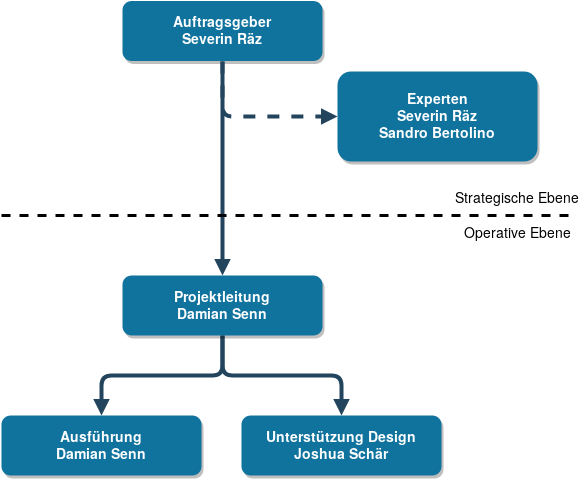
\includegraphics[width=0.8\textwidth]{figures/organigram.png}
  \caption{Organigram}
\end{figure}

\subsection{Tätigkeiten im Projekt}\label{tuxe4tigkeiten-im-projekt}

Für die Freigaben der Phasen ist nach Absprache mit Severin Räz Damian Senn
selbstständig verantwortlich.

\begin{longtable}[]{@{}ll@{}}
  \toprule
  \textbf{Name}    & \textbf{Funktions- und Tätigkeitsbereich}\tabularnewline
  \midrule
  \endhead
  Severin Räz      & Auftraggeber, externer Experte\tabularnewline
  Sandro Bertolino & Interner Experte\tabularnewline
  Damian Senn      & Projektleiter, Ausführung\tabularnewline
  Joshua Schär     & Unterstützung Design\tabularnewline
  \bottomrule
  \caption{Tätigkeiten Verteilung}
\end{longtable}

\subsection{Kommunikation}\label{kommunikation}

Wie im Kickoff-Meeting besprochen, wird Damian Senn alle zwei Wochen einen
kurzen Bericht an Sandro Bertolino und Severin Räz per E-Mail schicken.
Im Bericht wird erläutert was in der Zwischenzeit erledigt wurde und was
die nächsten Schritte im Projekt sind.

\clearpage

\section{Abgrenzungen}\label{abgrenzungen}

\begin{figure}[!htb]
  \centering
  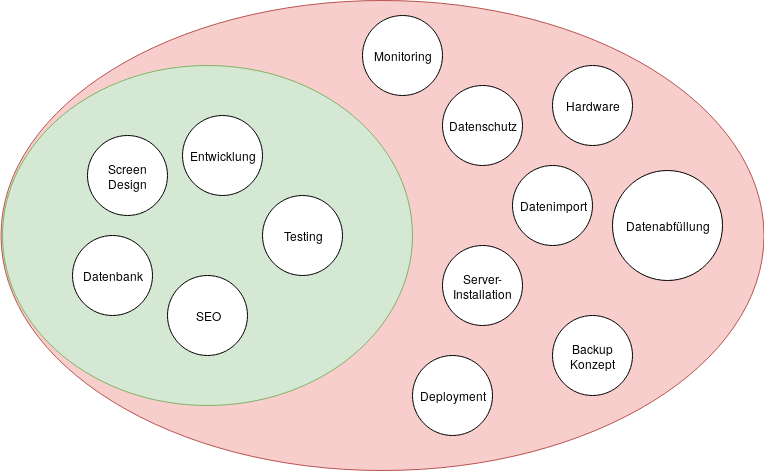
\includegraphics[width=0.95\textwidth]{figures/abgrenzungen.png}
  \caption{Abgrenzungen}
\end{figure}

\subsubsection{Hardware, Server-Installation, Deployment und
  Monitoring}\label{hardware-server-installation-deployment-und-monitoring}

Da das Projekt ein reines Software-Entwicklungs Projekt ist, werden
keine Operativen tätigkeiten wie Hardwarebeschaffung,
Server-Installation, Deployment und das einrichten eines
Monitoring-Systems vorgenommen.

\subsubsection{Datenschutz}\label{datenschutz}

Da das Projekt nicht deployed wird und somit nicht produktiv/online
gestellt wird, müssen im Rahmen dieser Projektarbeit noch keine Gedanken
über den Datenschutz gemacht werden.

\subsubsection{Datenimport}\label{datenimport}

Da wir bisher keine existierenden Konzertdaten besitzen, ist es nicht
nötig, einen Datenimport zu implementieren.

\subsubsection{Datenabfüllung}\label{datenabfuxfcllung}

Die Projektarbeit beinhaltet kein Datenset, Tests werden mit Testdaten
abgewickelt. Es liegt nicht in der Verantwortung des Projektleiters,
dass Daten in die Applikation abgefüllt werden.

\subsubsection{Backup Konzept}\label{backup-konzept}

Es wird kein Backup Konzept benötigt, da die Applikation im Rahmen
dieses Projektes nicht produktiv geschaltet wird.

\clearpage
\section{Anforderungskatalog}\label{anforderungskatalog}

Der Anforderungskatalog wurde in der Studie erarbeitet. Es wurden Kann und Muss
Kriterien definiert, wobei ein Muss-Kriterium zwingend erfüllt werden muss und
ein Kann-Kriterium als Erweiterung angesehen wird.

% TODO: Fix multirows across pages
%       https://tex.stackexchange.com/questions/79143/how-to-repeat-cell-content-on-next-page-for-longtable-using-multirow/79152
\begin{longtable}[]{@{}p{1.9cm}p{2.5cm}cp{5.5cm}cc@{}}
  \toprule
  \textbf{Feature}           & \textbf{Titel}             & \textbf{Nr.} & \textbf{Kriterium}                                                                                          & \textbf{Ziel} & \textbf{Muss}\tabularnewline
  \midrule
  \endhead
  \multirow{10}{*}{Suche}    & Suche nach Konzertname     & 1.1          & Listet alle Konzerte die Wörter der Suche im Konzertnamen beinhalten                                        & 1.1           & \textbf{Muss}                \\ \cline{2-6}
                             & Suche nach Konzertlocation & 1.2          & Schränkt die Such-Resultate nach gegebener Konzertlocation ein                                              & 1.2           & \textbf{Muss}                \\ \cline{2-6}
                             & Suche nach Ort             & 1.2          & Schränkt die Such-Resultate nach gegebenem Ort ein                                                          & 1.2           & \textbf{Muss}                \\ \cline{2-6}
                             & Suche nach Genre           & 1.2          & Schränkt die Such-Resultate nach gegebenem Musik-Genre ein                                                  & 1.2           & \textbf{Muss}                \\
  \midrule
  \multirow{8}{*}{Design}    & Desktop                    & 2.1          & Alle Ansichten haben eine Desktop-Optimierte Variante                                                       & 1.4           & \textbf{Muss}                \\ \cline{2-6}
                             & Tablet                     & 2.2          & Alle Ansichten haben eine Tablet-Optimierte Variante                                                        & 1.4           & \textbf{Muss}                \\ \cline{2-6}
                             & Mobile                     & 2.3          & Alle Ansichten haben eine Mobile-Optimierte Variante                                                        & 1.4           & \textbf{Muss}                \\ \cline{2-6}
                             & Browser Kompatibilität     & 2.4          & Alle Ansichten müssen in aktuellem Google Chrome und Mozilla Firefox dem Grundlayout folgen                 & 1.9           & \textbf{Muss}                \\
  \midrule
  \multirow{4}{*}{SEO}       & Indexierbarkeit            & 3.1          & Das Produkt ist von Suchmaschinen indexierbar                                                               & 1.5           & \textbf{Muss}                \\ \cline{2-6}
                             & Linked Data                & 3.2          & Konzert Detailseiten sind mit dem Event-Schema\footnote{\url{https://schema.org/Event}} ausgestattet              & 1.5           & \textbf{Muss}                \\
  \midrule
  \multirow{8}{*}{Benutzer}  & Registrierung              & 4.1          & Besucher können sich einen Benutzer registrieren, Benutzernamen und E-Mail Adressen müssen einzigartig sein & 1.6           & \textbf{Muss}                \\ \cline{2-6}
                             & Passwort-Vergessen         & 4.2          & Benutzer können sich einen Passwort-Reset Link anfordern                                                    & 1.7           & \textbf{Muss}                \\ \cline{2-6}
                             & Social                     & 4.3          & Benutzer können auf Konzerten vermerken ob sie Teilnehmen oder nicht                                        & 1.11          & Kann                         \\
  \midrule
  \clearpage
  \multirow{6}{*}{Erfassung} & Artist                     & 5.1          & Benutzer können Artisten mit einem Genre erfassen                                                           & 1.8           & \textbf{Muss}                \\ \cline{2-6}
                             & Location                   & 5.2          & Benutzer können eine Konzertlocation mit Ort/Strasse erfassen                                               & 1.8           & \textbf{Muss}                \\ \cline{2-6}
                             & Konzert                    & 5.3          & Benutzer können ein Konzert mit Konzertlocation und Artisten erfassen                                       & 1.8           & \textbf{Muss}                \\ \cline{2-6}
                             & Facebook                   & 5.4          & Benutzer können ein Konzert in ein Facebook-Event exportieren                                               & 1.10          & Kann                         \\
  \midrule
  \multirow{9}{*}{Security}  & SQL-Injection              & 6.1          & Das Produkt soll resistent gegen SQL-Injection sein                                                         & 1.12          & \textbf{Muss}                \\ \cline{2-6}
                             & HTML-Injection             & 6.2          & Das Produkt soll resistent gegen HTML-Injection / XSS sein                                                  & 1.12          & \textbf{Muss}                \\ \cline{2-6}
                             & Passwort encryption        & 6.3          & Passwörter von Benutzer müssen mit einem sicheren Verfahren gespeichert werden                              & 1.12          & \textbf{Muss}                \\ \cline{2-6}
                             & Session                    & 6.4          & Session-Cookies dürfen nicht durch JavaScript ausgelesen werden                                             & 1.12          & Kann                         \\
  \midrule
  Performance                & Ladezeit                   & 7.1          & Die Seitenansichten dürfen nicht länger als 6 Sekunden auf einem 3G Netz laden                              &               & \textbf{Muss}                \\
  \midrule
  Sonstiges                  & User Tracking              & 8.1          & Benutzerverhalten soll analysiert und nachvollziehbar sein.                                                 &               & Kann                         \\
  \bottomrule
  \caption{Anforderungskatalog}
\end{longtable}


\clearpage
\section{Lösungsbeschreibung}\label{loesungsbeschreibung}

In der Studie (Anhang~\ref{AppendixStudie}) wurden Technologien gegenüber
gestellt und für die Umsetzung mittels Nutzwertanalysen ausgewählt.\\

\noindent
Folgende Technologien wurden ausgewählt:\\

\textbf{Browser sowie Server Technologie:}

\begin{figure}[!htb]
  \centering
  
\includegraphics[width=0.8\textwidth]{figures/phoenix.png}
  \captionsource{Phoenix Framework Logo}{\url{https://github.com/phoenixframework/phoenix}}
\end{figure}

\noindent
Die Nutzwertanalyse hat ergeben, dass es sinnvoller ist, das Projekt mit
einer klassischen SSR Applikation zu starten. Das Phoenix Framework bietet alle
benötigten Features an und kann durch zusätzliche Module einfach erweitert werden.

Für dynamische Interaktionen wie Formular-Validierungen wird zu einfachem
JavaScript gegriffen. Ist ein Screen besonders interaktiv, kann gegebenenfalls
eine kleinere JavaScript-Library verwendet werden um die Problemlösung zu
vereinfachen.\\

\textbf{Testing Technologie:}

\begin{figure}[!htb]
  \centering
  
\includegraphics[width=0.8\textwidth]{figures/wallaby.png}
  \captionsource{Wallaby Logo}{\url{https://github.com/keathley/wallaby}}
\end{figure}

\noindent
Getestet wird die Applikation durch die von Phoenix gegebenen Testing-Tools
sowie mit der Browser-Testing Library «Wallaby».

\clearpage
\section{Kosten}\label{projektauftragkosten}

In der Studie wurden die Projekt- sowie Betriebskosten ausgerechnet.

Der gesamte Personalaufwand beträgt \textbf{42'900} für die geplanten Stunden.

\begin{longtable}[]{@{}lrr@{}}
  \toprule
  \textbf{Phase}  & \makecell[r]{\textbf{Geplante} \\\textbf{Stunden}} & \textbf{Kosten}\tabularnewline
  \midrule
  \endhead
  Initialisierung &  64                       &  9'600.- CHF\tabularnewline
  Konzept         &  66                       &  9'900.- CHF\tabularnewline
  Realisierung    & 136                       & 20'400.- CHF\tabularnewline
  Abschluss       &  64                       &  5'400.- CHF\tabularnewline
  \midrule
  \textbf{Total:} & 286                       & 42'900.- CHF\tabularnewline
  \bottomrule
  \caption{Projektkosten}
\end{longtable}


Für die Betriebskosten wurde angenommen, dass das Produkt in der Cloud auf
einer mittelgrossen Umgebung betrieben wird. Die Kosten dieser Umgebung wurde
auf 150.- CHF pro Monat geschätzt.

Neben der Umgebung muss mindestens eine Domain gekauft und jährlich bezahlt
werden. Die Kosten einer Domain sind rund 20.- CHF pro Jahr.

Da jediglich Open Source Software eingesetzt wird, gibt es keine
Software-Lizenzen zu bezahlen.

\begin{longtable}[]{@{}lll@{}}
  \toprule
  \textbf{Kostenstelle} & \textbf{Jährliche Kosten}\tabularnewline
  \midrule
  \endhead
  Software              & Keine\tabularnewline
  .com Domain           & 20.- CHF\tabularnewline
  Hosting               & 1'800.- CHF\tabularnewline
  \midrule
  \textbf{Total:}       & 1'820.- CHF\tabularnewline
  \bottomrule
  \caption{Betriebskosten}
\end{longtable}


\clearpage
\section{Risiken}\label{risiken}

Die Risikobewertung erfolgt mit folgender Formel:\\

\textbf{Bewertung = Schaden x Eintrittswahrscheinlichkeit}\\

\noindent
Schadensskala:

\begin{longtable}[]{@{}lp{11cm}@{}}
  \toprule
  \textbf{Gewichtung} & \textbf{Beschreibung}\tabularnewline
  \midrule
  \endhead
  Gering (1-2)        & Kleiner Schaden, hat kaum Auswirkungen auf das Projekt.\tabularnewline
  Mittel (3-4)        & Mittlerer Schaden, Zeitverzögerungen oder Qualitätsverluste.\tabularnewline
  Hoch (5-6)          & Hoher Schaden, wichtige Arbeiten oder Phasen können nicht abgeschlossen werden, schlimmstenfalls ein Abbruch des Projekts.\tabularnewline
  \bottomrule
  \caption{Risiken - Schadensskala}
\end{longtable}

\noindent
Eintrittswahrscheinlichkeitsskala:

\begin{longtable}[]{@{}lp{12cm}@{}}
  \toprule
  \textbf{Gewichtung} & \textbf{Beschreibung}\tabularnewline
  \midrule
  \endhead
  Gering (1-2)        & Kleine Eintrittswahrscheinlichkeit.\tabularnewline
  Mittel (3-4)        & Mittlere Eintrittswahrscheinlichkeit.\tabularnewline
  Hoch (5-6)          & Hohe Eintrittswahrscheinlichkeit.\tabularnewline
  \bottomrule
  \caption{Risiken - Eintrittswahrscheinlichkeit}
\end{longtable}

\noindent
Handlungen um Risikobewertungen zu senken:

\begin{longtable}[]{@{}lp{12cm}@{}}
  \toprule
  \textbf{Handlung} & \textbf{Beschreibung}\tabularnewline
  \midrule
  \endhead
  Akzeptanz         & Das Eintreten eines Risiko wird wissentlich angenommen.\tabularnewline
  Transfer          & Die Verantwortung von Risiken können an Dritte abgegeben werden.\tabularnewline
  Verminderung      & Der Schaden oder die Eintrittswahrscheinlichkeit kann begrenzt oder reduziert werden.\tabularnewline
  Vermeidung        & Es kann jeglichen Schaden vermieden werden.\tabularnewline
  \bottomrule
  \caption{Risiken - Handlungen zur Senkung der Bewertung}
\end{longtable}


\clearpage
\subsection{Projektrisiken}\label{projektrisiken}

\begin{longtable}[]{@{}lp{3cm}p{4cm}ccc@{}}
  \toprule
  \textbf{Nr.} & \textbf{Risiko}                             & \textbf{Auswirkung}                                 & \textbf{Schaden} & \textbf{Wahrsch.} & \textbf{Bewertung}\tabularnewline
  \midrule
  \endhead
  1            & Ausfall des Entwicklers oder Projektleiters & Verzögerungen von Arbeiten                          & 4                & 3                 & Mittel\tabularnewline
  2            & Unvollständige Projektdokumentation         & Schlechtere Diplomarbeit Bewertung                  & 4                & 2                 & Mittel\tabularnewline
  3            & Schlechter Projektplan                      & Verzögerungen und eventuelle Qualitätsverluste      & 4                & 3                 & Mittel\tabularnewline
  4            & Keine Benutzer                              & Das Produkt wird nicht von Benutzern eingesetzt     & 3                & 4                 & Mittel\tabularnewline
  5            & Technisch nicht umsetzbare Features         & Das Produkt kann nicht wie angedacht benutzt werden & 4                & 3                 & Mittel\tabularnewline
  \bottomrule
  \caption{Projektrisiken}
\end{longtable}

\clearpage
\subsection{Massnahmen}\label{massnahmen}

\begin{longtable}[]{@{}lp{4.1cm}lccc@{}}
  \toprule
               &                                                                       &                   & \multicolumn{3}{l}{\textbf{Bewertung nach Massnahme}}\tabularnewline
  \textbf{Nr.} & \textbf{Massnahme}                                                    & \textbf{Handlung} & \textbf{Schaden}                                                     & \textbf{Wahrsch.} & \textbf{Bewertung}\tabularnewline
  \midrule
  \endhead
  1            & Arzt aufsuchen, ggf. Projekt-Pause oder Abbruch                       & Akzeptanz         & 4                                                                    & 3                 & Mittel\tabularnewline
  2            & Statusbericht alle zwei Wochen, bei Fragen sofort Hilfe suchen        & Verminderung      & 2                                                                    & 1                 & Gering\tabularnewline
  3            & Genügend Buffer-Zeit einplanen, ggf. Ferientage für Projekt einsetzen & Verminderung      & 2                                                                    & 1                 & Gering\tabularnewline
  4            & Das Produkt löst vor allem ein persönliches Interesse                 & Akzeptanz         & 3                                                                    & 4                 & Mittel\tabularnewline
  5            & Vereinfachte Alternativen in Konzept-Phase untersuchen                & Verminderung      & 2                                                                    & 2                 & Gering\tabularnewline
  \bottomrule
  \caption{Projektrisiken - Massnahmen}
\end{longtable}

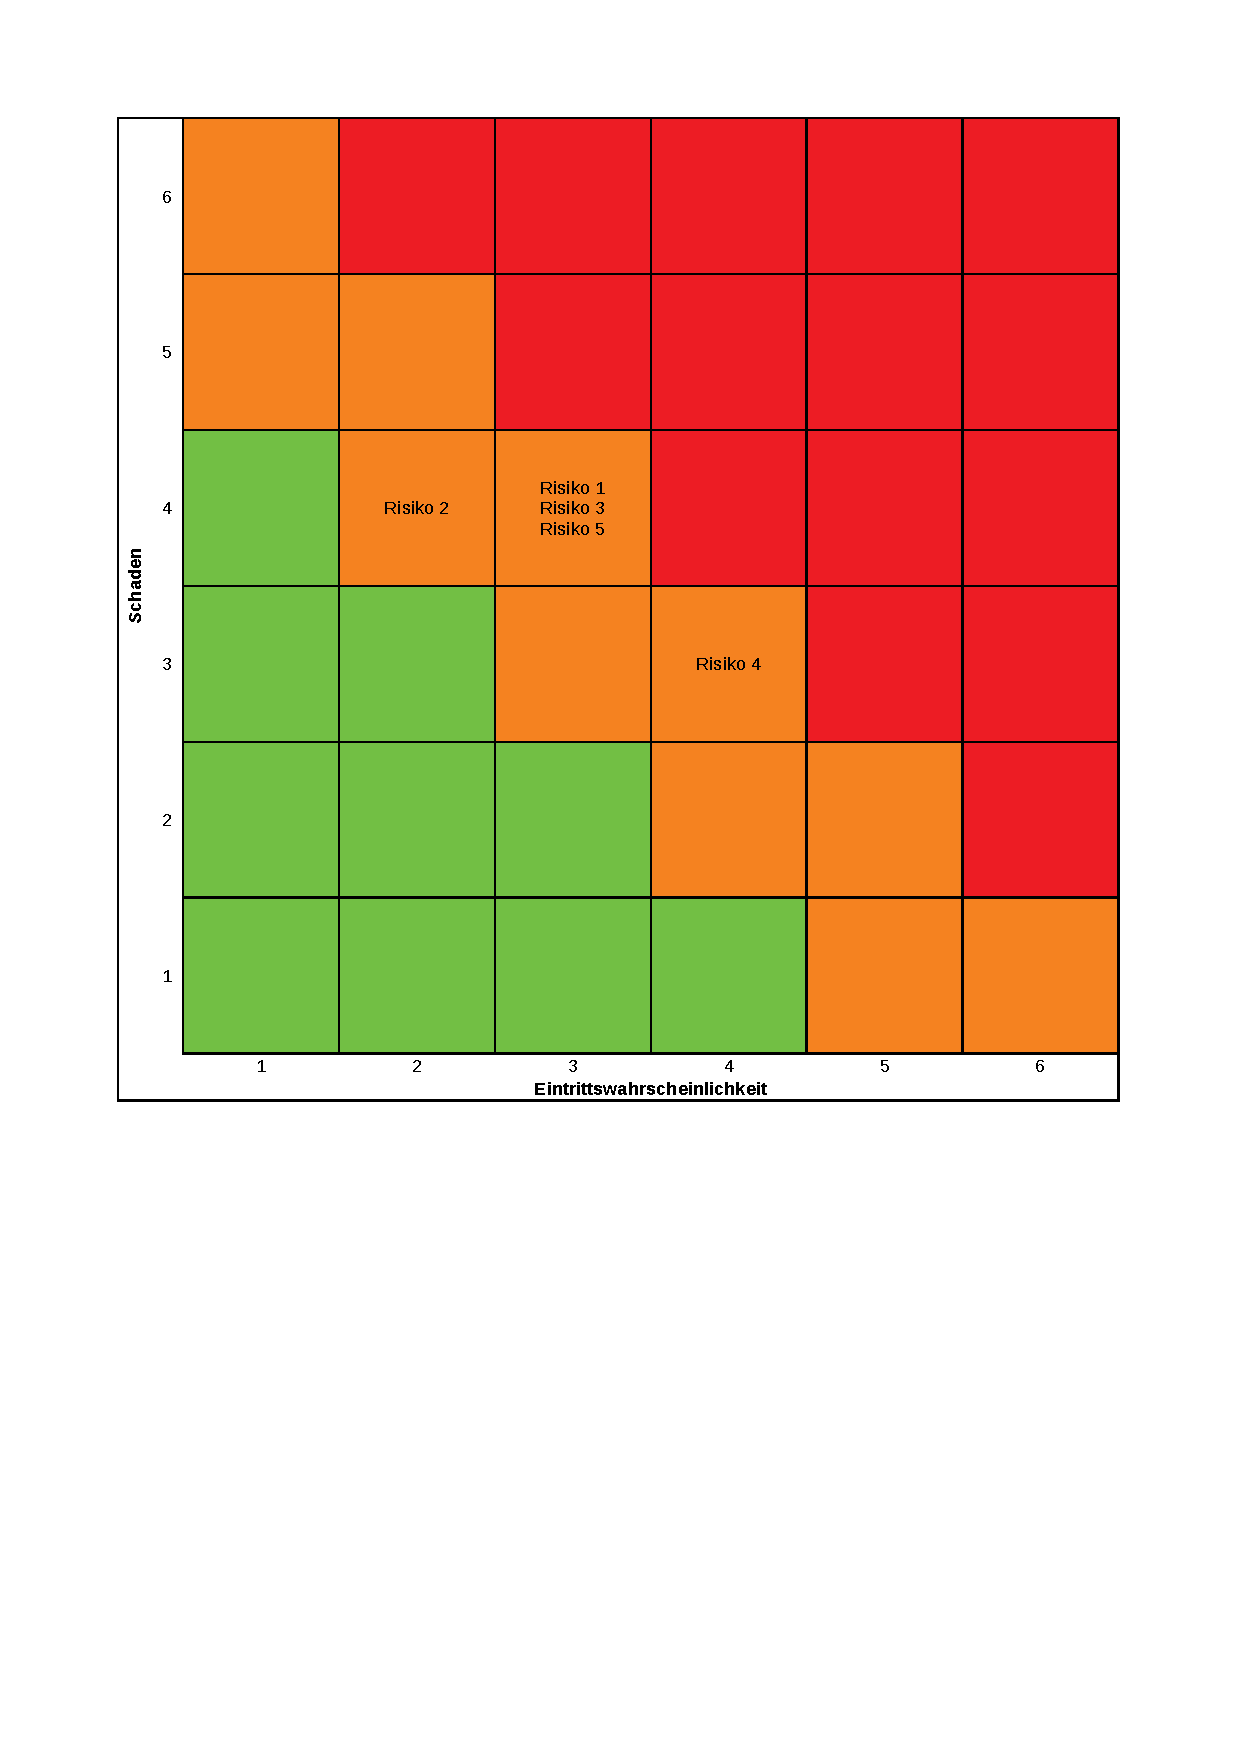
\includepdf[pages=1, pagecommand={\subsection{Risikodiagramm ohne Massnahmen}\label{risikodiagram-ohne-massnahmen}}, trim=0mm 80mm 0mm 0mm, clip]{initialisierung/risiko.pdf}
\includepdf[pages=2, pagecommand={\subsection{Risikodiagramm mit Massnahmen}\label{risikodiagram-mit-massnahmen}}, trim=0mm 80mm 0mm 0mm, clip]{initialisierung/risiko.pdf}

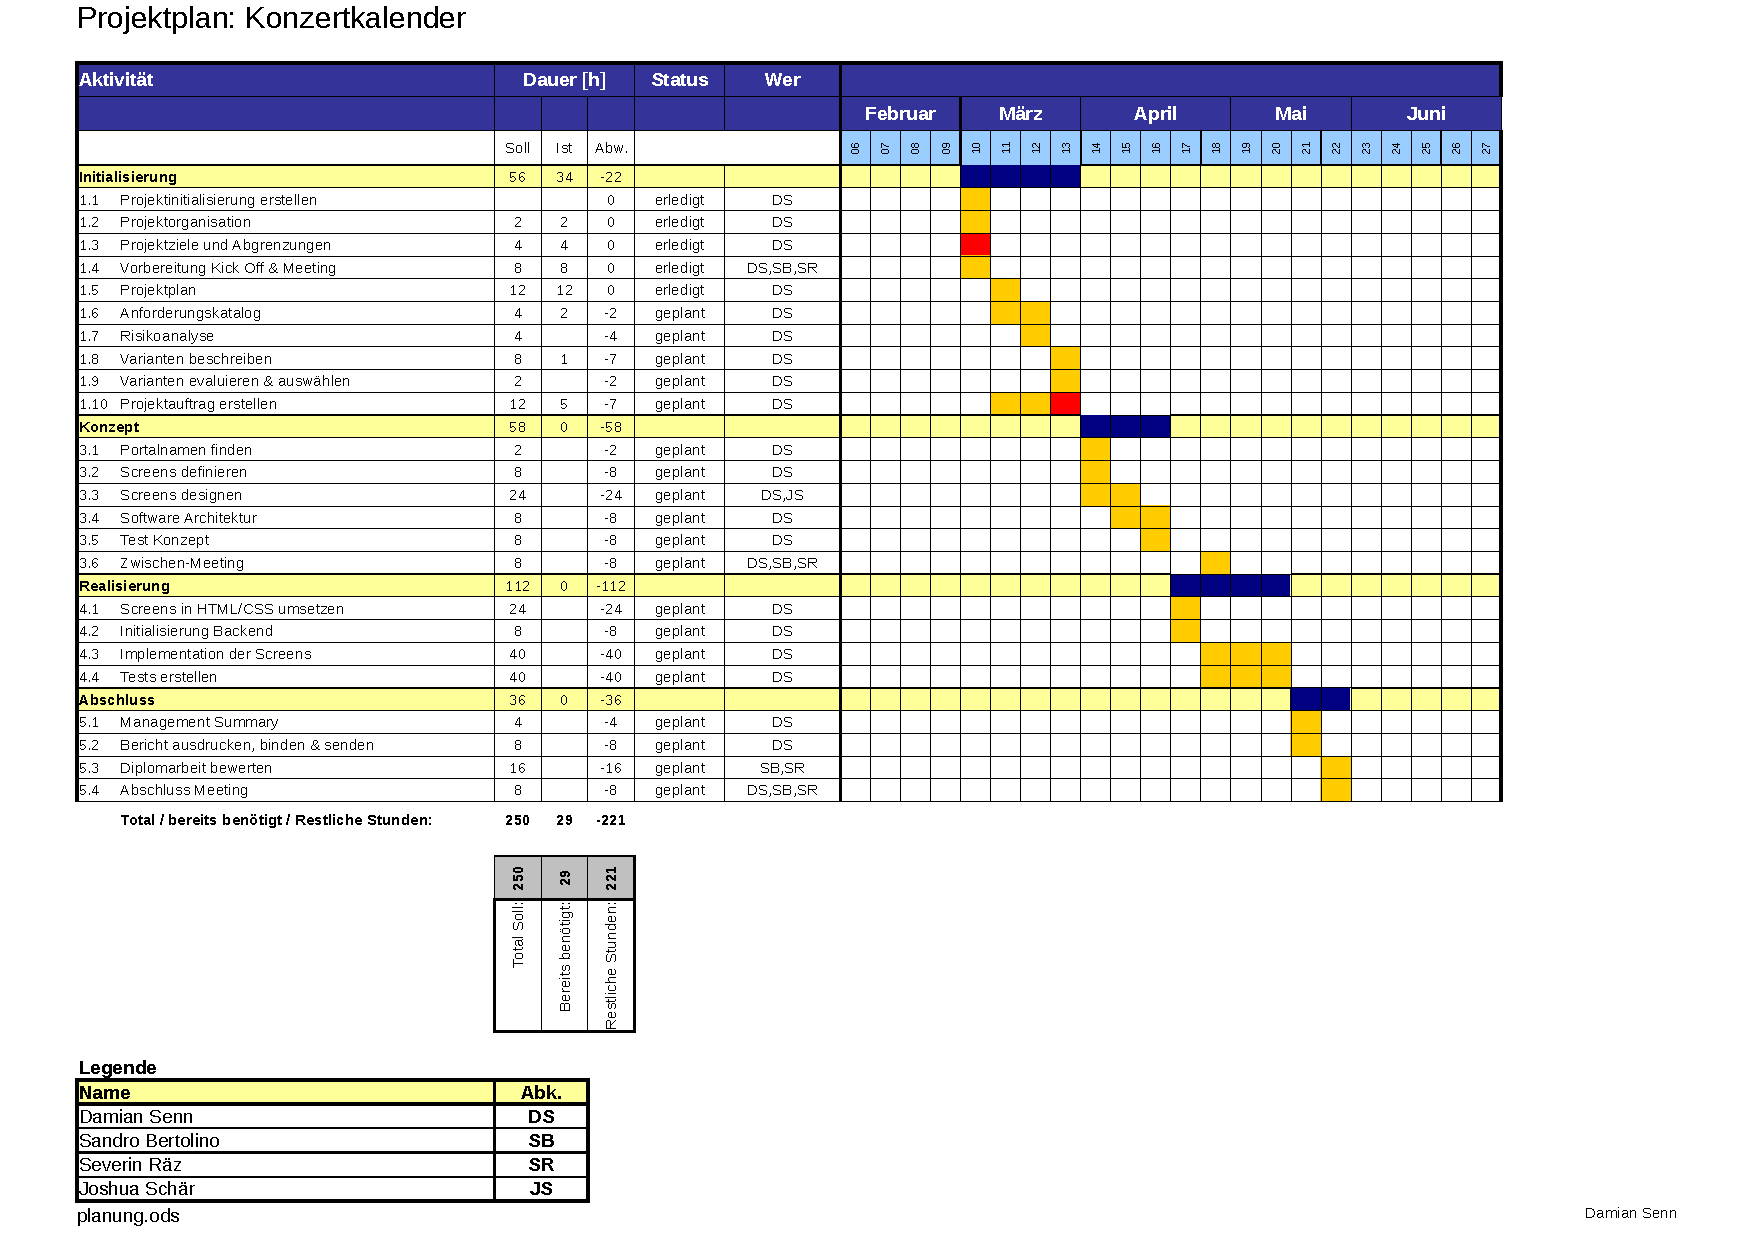
\includepdf[pagecommand={\chapter{Terminplan}\label{terminplan}}]{initialisierung/planung.pdf}
\chapter{Studie}

\label{AppendixStudie}

\section{Zweck des Dokuments}\label{StudieZweck}

In der Studie werden die Anforderungen aufgenommen, sowie Variantenbeschriebe
für die Projektrealisierung erstellt. Die Varianten werden miteinander
verglichen und durch den Variantenentscheid wird das weitere
Vorgehen definiert.
Ausserdem werden in der Studie die Risiken und Wirtschaftlichkeit des Projekts
analysiert.

Folgende Arbeiten werden in dieser Studie abgehandelt:

\begin{itemize}
  \tightlist
  \item der Anforderungskatalog wird definiert
  \item die Evaluation der Browser Software-Technologien
  \item die Evaluation der Server Software-Technologien
  \item die Evaluation der Testing Software-Technologien
  \item eine Kostenschätzung und mögliche Wirtschaftlichkeit ausgerechnet
\end{itemize}


\section{Informationsbeschaffung}\label{informationsbeschaffung}

\begin{longtable}[]{@{}lp{10cm}@{}}
  \toprule
  Quelle                        & Beschreibung\tabularnewline
  \toprule
  Schulwissen / Berufserfahrung & Die Grundlage für die Umsetzung dieses Projekts wird durch mein existierendes Schulwissen sowie meine langjährige Berufserfahrung in der Software-Entwicklung gesetzt.\tabularnewline
  \midrule
  Internet                      & Ein Grossteil der Informationen werden heute über das Internet bezogen, für die Evaluation von Technologien und Lösungsansätzen wird einiges über das Internet recherchiert werden müssen.\tabularnewline
  \bottomrule
  \caption{Informationsbeschaffung}
\end{longtable}

\clearpage
\section{Anforderungskatalog}\label{anforderungskatalog}

% TODO: Fix multirows across pages
%       https://tex.stackexchange.com/questions/79143/how-to-repeat-cell-content-on-next-page-for-longtable-using-multirow/79152
\begin{longtable}[]{@{}p{1.9cm}p{2.5cm}cp{5.5cm}cc@{}}
  \toprule
  \textbf{Feature}           & \textbf{Titel}             & \textbf{Nr.} & \textbf{Kriterium}                                                                                          & \textbf{Ziel} & \textbf{Muss}\tabularnewline
  \midrule
  \endhead
  \multirow{10}{*}{Suche}    & Suche nach Konzertname     & 1.1          & Listet alle Konzerte die Wörter der Suche im Konzertnamen beinhalten                                        & 1.1           & \textbf{Muss}                \\ \cline{2-6}
                             & Suche nach Konzertlocation & 1.2          & Schränkt die Such-Resultate nach gegebener Konzertlocation ein                                              & 1.2           & \textbf{Muss}                \\ \cline{2-6}
                             & Suche nach Ort             & 1.2          & Schränkt die Such-Resultate nach gegebenem Ort ein                                                          & 1.2           & \textbf{Muss}                \\ \cline{2-6}
                             & Suche nach Genre           & 1.2          & Schränkt die Such-Resultate nach gegebenem Musik-Genre ein                                                  & 1.2           & \textbf{Muss}                \\
  \midrule
  \multirow{8}{*}{Design}    & Desktop                    & 2.1          & Alle Ansichten haben eine Desktop-Optimierte Variante                                                       & 1.4           & \textbf{Muss}                \\ \cline{2-6}
                             & Tablet                     & 2.2          & Alle Ansichten haben eine Tablet-Optimierte Variante                                                        & 1.4           & \textbf{Muss}                \\ \cline{2-6}
                             & Mobile                     & 2.3          & Alle Ansichten haben eine Mobile-Optimierte Variante                                                        & 1.4           & \textbf{Muss}                \\ \cline{2-6}
                             & Browser Kompatibilität     & 2.4          & Alle Ansichten müssen in aktuellem Google Chrome und Mozilla Firefox dem Grundlayout folgen                 & 1.9           & \textbf{Muss}                \\
  \midrule
  \multirow{4}{*}{SEO}       & Indexierbarkeit            & 3.1          & Das Produkt ist von Suchmaschinen indexierbar                                                               & 1.5           & \textbf{Muss}                \\ \cline{2-6}
                             & Linked Data                & 3.2          & Konzert Detailseiten sind mit dem Event-Schema\footnote{\url{https://schema.org/Event}} ausgestattet              & 1.5           & \textbf{Muss}                \\
  \midrule
  \multirow{8}{*}{Benutzer}  & Registrierung              & 4.1          & Besucher können sich einen Benutzer registrieren, Benutzernamen und E-Mail Adressen müssen einzigartig sein & 1.6           & \textbf{Muss}                \\ \cline{2-6}
                             & Passwort-Vergessen         & 4.2          & Benutzer können sich einen Passwort-Reset Link anfordern                                                    & 1.7           & \textbf{Muss}                \\ \cline{2-6}
                             & Social                     & 4.3          & Benutzer können auf Konzerten vermerken ob sie Teilnehmen oder nicht                                        & 1.11          & Kann                         \\
  \midrule
  \clearpage
  \multirow{6}{*}{Erfassung} & Artist                     & 5.1          & Benutzer können Artisten mit einem Genre erfassen                                                           & 1.8           & \textbf{Muss}                \\ \cline{2-6}
                             & Location                   & 5.2          & Benutzer können eine Konzertlocation mit Ort/Strasse erfassen                                               & 1.8           & \textbf{Muss}                \\ \cline{2-6}
                             & Konzert                    & 5.3          & Benutzer können ein Konzert mit Konzertlocation und Artisten erfassen                                       & 1.8           & \textbf{Muss}                \\ \cline{2-6}
                             & Facebook                   & 5.4          & Benutzer können ein Konzert in ein Facebook-Event exportieren                                               & 1.10          & Kann                         \\
  \midrule
  \multirow{9}{*}{Security}  & SQL-Injection              & 6.1          & Das Produkt soll resistent gegen SQL-Injection sein                                                         & 1.12          & \textbf{Muss}                \\ \cline{2-6}
                             & HTML-Injection             & 6.2          & Das Produkt soll resistent gegen HTML-Injection / XSS sein                                                  & 1.12          & \textbf{Muss}                \\ \cline{2-6}
                             & Passwort encryption        & 6.3          & Passwörter von Benutzer müssen mit einem sicheren Verfahren gespeichert werden                              & 1.12          & \textbf{Muss}                \\ \cline{2-6}
                             & Session                    & 6.4          & Session-Cookies dürfen nicht durch JavaScript ausgelesen werden                                             & 1.12          & Kann                         \\
  \midrule
  Performance                & Ladezeit                   & 7.1          & Die Seitenansichten dürfen nicht länger als 6 Sekunden auf einem 3G Netz laden                              &               & \textbf{Muss}                \\
  \midrule
  Sonstiges                  & User Tracking              & 8.1          & Benutzerverhalten soll analysiert und nachvollziehbar sein.                                                 &               & Kann                         \\
  \bottomrule
  \caption{Anforderungskatalog}
\end{longtable}


\clearpage
\section{Evaluation Browser-Technologie}\label{evaluation-browser-technologie}

\begin{longtable}[]{@{}p{2cm}cp{10cm}@{}}
  \toprule
  \textbf{Kriterium} & \textbf{Gewicht} & \textbf{Abnahmekriterium}\tabularnewline
  \midrule
  \endhead
  Komplexität        & 3                & Die Technologie sollte im Rahmen der Diplomarbeit nicht eine zu hohe Komplexität vorweisen. Durch eine niedrigere Komplexität bestehen weniger Risiken dass technische Probleme auftreten werden.\tabularnewline
  \midrule
  Performance        & 4                & In den Projektzielen wurde definiert, dass die Applikation in maximal 6 Sekunden im Browser geladen sein muss. Daher ist es wichtig, dass die Technologie gute Performance Charakteristiken vorweist.\tabularnewline
  \midrule
  SEO                & 5                & Für eine öffentliche Applikation ist es unentbehrlich, dass sie indexierbar durch Suchmaschinen ist.\tabularnewline
  \midrule
  Interaktivität     & 4                & Applikationen im Browser werden immer interaktiver, daher ist es wichtig, das die Technologie anspruchsvolle Abläufe implementieren kann. \tabularnewline
  \midrule
  Stabilität         & 3                & Für das Projekt ist es wichtig, dass auf eine stabile Technologie gesetzt wird, welche den Projektablauf so wenig wie möglich beeinträchtigt. \tabularnewline
  \midrule
  Testing            & 3                & Durch einfaches Testing, kann sichergestellt werden, dass die Applikation wie gewünscht umgesetzt wurde und auch beim Weiterentwickeln nicht existierende Funktionalitäten beinträchtigt werden.\tabularnewline
  \bottomrule
  \caption{Browser-Technologie Kriterien}
\end{longtable}

\subsection{Variante: React}

Die JavaScript Library \textbf{React} ist heute die wohl beliebteste
Technologie um interaktive Applikationen im Web zu bauen.

\subsection{Variante: Next.js}

\textbf{Next.js} ist ein JavaScript Framework, das auf der \textbf{React}
Library aufbaut und zusätzliche Features sowie gängige Konventionen mitbringt.

\subsection{Variante: SSR}

\textbf{SSR} steht für \textbf{S}erver\textbf{s}ide \textbf{R}endering und
beschreibt die klassische Methode vom Erstellen von Webseiten, indem man HTML
auf dem Server generiert und zum Browser schickt.

Dies hat nach wie vor seine Daseinsberechtigung, da dies weniger Komplexität
mit sich bringt, einen schnelleren Seitenaufbau garantiert und ohne
zusätzlichen Aufwand von Suchmaschinen indexiert wird.

\clearpage
\section{Bewertungen Browser-Technologie}\label{bewertungen-browser-technologie}

\textbf{Bewertung:}\\
\textit{4 = Sehr gut, 3 = Gut, 2 = Ungenügend, 1 = Schlecht}\\
\textbf{Gewichtung:}\\
\textit{5 = Unverzichtbar, 4 = Sehr wichtig, 3 = Erleichtert die Arbeit, 2 = Weniger wichtig, 1 = unwichtig}\\

\textbf{\textit{Bewertung x Gewichtung = Punktzahl}}

\begin{longtable}[]{@{}p{2cm}ccccccc@{}}
  \toprule
  \textbf{Kriterium} & \textbf{Gewichtung} & \multicolumn{2}{c}{\textbf{Variante: React}} & \multicolumn{2}{c}{\textbf{Variante: Next.js}} & \multicolumn{2}{c}{\textbf{Variante: SSR}}\tabularnewline
                     &                     & Bewertung                                    & Punkte                                         & Bewertung                                                 & Punkte & Bewertung & Punkte \tabularnewline
  \midrule
  \endhead
  Komplexität        & 3                   & 2                                            & 6                                              & 3                                                         & 9      & 4         & 12 \tabularnewline
  Performance        & 4                   & 3                                            & 12                                             & 3                                                         & 12     & 4         & 16 \tabularnewline
  SEO                & 5                   & 2                                            & 10                                             & 4                                                         & 20     & 4         & 20 \tabularnewline
  Interaktivität     & 4                   & 4                                            & 16                                             & 4                                                         & 16     & 3         & 12 \tabularnewline
  Stabilität         & 3                   & 2                                            & 6                                              & 3                                                         & 9      & 4         & 12 \tabularnewline
  Testing            & 4                   & 4                                            & 16                                             & 4                                                         & 16     & 4         & 16 \tabularnewline
  \midrule
  \textbf{Total:}    &                     & React:                                       & 66                                             & Next.js:                                                  & 82     & SSR:      & 88 \tabularnewline
  \bottomrule
  \caption{Browser-Technologie Bewertung}
\end{longtable}

\section{Entscheid Browser-Technologie}\label{entscheid-browser-technologie}

Durch die Evaluierung wurde klar, dass das Einsetzen eines JavaScript-Frameworks
zuviel zusätzliche Komplexität und gewisse einbussungen in Performance und Stabilität
unvermeidbar ist. Somit ist ein die Wahl für eine klassische Server-Side Rendered
Webseite favorisierend.

Es ist durchaus vorstellbar, dass in einem zweiten Schritt, nach diesem Projekt,
die Server-Side Rendered Applikation durch eine Next.js Applikation ersetzt werden
könnte.

\clearpage
\section{Evaluation Server-Technologie}\label{evaluation-server-technologie}

\begin{longtable}[]{@{}p{2cm}cp{10cm}@{}}
  \toprule
  \textbf{Kriterium} & \textbf{Gewicht} & \textbf{Abnahmekriterium}\tabularnewline
  \midrule
  \endhead
  Komplexität        & 3                & Die Technologie sollte im Rahmen der Diplomarbeit nicht eine zu hohe Komplexität vorweisen. Durch eine niedrigere Komplexität bestehen weniger Risiken dass technische Probleme auftreten werden.\tabularnewline
  \midrule
  Performance        & 4                & In den Projektzielen wurde definiert, dass die Applikation in maximal 6 Sekunden im Browser geladen sein muss. Daher ist es wichtig, dass die Technologie gute Performance Charakteristiken vorweist.\tabularnewline
  \midrule
  Stabilität         & 5                & Während es für die Browser-Technologie vorstellbar ist, die Technologie auszuwechseln, ist es für den Server wichtig auf eine stabile und zukunftssichere Technologie zu setzen.\tabularnewline
  \midrule
  Testing            & 5                & Durch einfaches Testing, kann sichergestellt werden, dass die Applikation wie gewünscht umgesetzt wurde und auch beim Weiterentwickeln nicht existierende Funktionalitäten beinträchtigt werden. Vorallem auf dem Server ist wichtig, dass die Businesslogik gut abdeckend gestestet werden kann.\tabularnewline
  \bottomrule
  \caption{Server-Technologie Kriterien}
\end{longtable}

\subsection{Variante: Node.js / koa.js}

Auch auf dem Server gewinnt JavaScript immer mehr an Beliebtheit.
Mit Node.js und koa.js können schnell kleinere und simplere Applikationen
erstellt werden, die dennoch sehr performant sind.

\subsection{Variante: Elixir / Phoenix}

Elixir ist eine Programmiersprache die eine sehr stabile und performante Grundlage
bietet. Durch das Framework Phoenix, wird im Elixir Ökosystem ein starkes feature
umfangreiches Web-Framework angeboten.

\subsection{Variante: Next.js}

Next.js wurde bereits als Variante für die Browser-Technologie in Betracht
gezogen. Ein zusätzliches Feature von Next.js ist, dass die Applikation auch
auf dem Server betrieben werden kann.
Das Einsetzen der selben Technologie kann bedeutende Vorteile mit sich bringen,
so muss man nur ein Framework lernen und kann Programmcode auf dem Server mit
der Applikation im Browser geteilt werden.

\clearpage
\section{Bewertungen Server-Technologie}\label{bewertungen-server-technologie}

\textbf{Bewertung:}\\
\textit{4 = Sehr gut, 3 = Gut, 2 = Ungenügend, 1 = Schlecht}\\
\textbf{Gewichtung:}\\
\textit{5 = Unverzichtbar, 4 = Sehr wichtig, 3 = Erleichtert die Arbeit, 2 = Weniger wichtig, 1 = unwichtig}\\

\textbf{\textit{Bewertung x Gewichtung = Punktzahl}}

\begin{longtable}[]{@{}p{2cm}ccccccc@{}}
  \toprule
  \textbf{Kriterium} & \textbf{Gewichtung} & \multicolumn{2}{c}{\textbf{Variante: koa.js}} & \multicolumn{2}{c}{\textbf{Variante: Phoenix}} & \multicolumn{2}{c}{\textbf{Variante: Next.js}}\tabularnewline
                     &                     & Bewertung                                     & Punkte                                         & Bewertung                                                     & Punkte & Bewertung & Punkte \tabularnewline
  \midrule
  \endhead
  Komplexität        & 3                   & 2                                             & 6                                              & 4                                                             & 12     & 3         & 9 \tabularnewline
  Performance        & 4                   & 4                                             & 16                                             & 4                                                             & 16     & 3         & 12 \tabularnewline
  Stabilität         & 5                   & 3                                             & 15                                             & 4                                                             & 20     & 3         & 15 \tabularnewline
  Testing            & 5                   & 3                                             & 15                                             & 4                                                             & 20     & 4         & 20 \tabularnewline
  \midrule
  \textbf{Total:}    &                     & koa.js:                                       & 55                                             & Phoenix:                                                      & 68     & Next.js:  & 56 \tabularnewline
  \bottomrule
  \caption{Server-Technologie Bewertung}
\end{longtable}

\section{Entscheid Server-Technologie}\label{entscheid-server-technologie}

Durch das grosse Featureste von Phoenix sowie tiefer Komplexität gegenüber den
beiden anderen Varianten hat sich Phoenix für die Server-Technologie ganz klar
durchgesetzt.

\clearpage
\section{Evaluation Testing-Technologie}\label{evaluation-testing-technologie}

\begin{longtable}[]{@{}p{2cm}cp{10cm}@{}}
  \toprule
  \textbf{Kriterium}  & \textbf{Gewicht} & \textbf{Abnahmekriterium}\tabularnewline
  \midrule
  \endhead
  Performance         & 3                & Bei wachsender Anzahl von Tests ist es wichtig, dass die Test-Software genug skalierbar ist um Tests in parallel auszuführen.\tabularnewline
  \midrule
  Stabilität          & 5                & \tabularnewline
  \midrule
  Backend-Integration & 4                & Es ist sehr hilfreich, wenn die End-to-End Test-Software vom Server direkt ausgeführt werden. So kann gleichzeitig zum Browser-Test auch die Businesslogik getestet werden.\tabularnewline
  \midrule
  Visualtesting       & 5                & Die Technologie soll mit dem Service percy.io integrierbar sein.\tabularnewline
  \bottomrule
  \caption{Testing-Technologie Kriterien}
\end{longtable}

\subsection{Jest + Puppeteer}

Jest ist ein JavaScript-Test Framework von Facebook. Durch die Kombinierung der
Puppeteer Library von Google ist es möglich, automatisierte Browser-Tests
durchzuführen.

\subsection{Wallaby}

Wallaby ist ein Elixir Browser-Test Framework, welches sich nahtlos mit Phoenix
integrieren lässt. Wallaby unterstützt parallelisierung von Tests und ist daher
ein guter Kanditat eine hohe Anzahl von automatisierten Tests.

\clearpage
\section{Bewertungen Testing-Technologie}\label{bewertungen-testing-technologie}

\textbf{Bewertung:}\\
\textit{4 = Sehr gut, 3 = Gut, 2 = Ungenügend, 1 = Schlecht}\\
\textbf{Gewichtung:}\\
\textit{5 = Unverzichtbar, 4 = Sehr wichtig, 3 = Erleichtert die Arbeit, 2 = Weniger wichtig, 1 = unwichtig}\\

\textbf{\textit{Bewertung x Gewichtung = Punktzahl}}

\begin{longtable}[]{@{}p{2cm}ccccc@{}}
  \toprule
  \textbf{Kriterium}  & \textbf{Gewichtung} & \multicolumn{2}{c}{\textbf{Variante: Jest}} & \multicolumn{2}{c}{\textbf{Variante: Wallaby}}\tabularnewline
                      &                     & Bewertung                                   & Punkte                                                        & Bewertung & Punkte\tabularnewline
  \midrule
  \endhead
  Performance         & 3                   & 4                                           & 12                                                            & 4         & 12\tabularnewline
  Stabilität          & 5                   & 3                                           & 15                                                            & 4         & 20\tabularnewline
  Backend-Integration & 4                   & 2                                           & 8                                                             & 4         & 16\tabularnewline
  Visualtesting       & 4                   & 4                                           & 16                                                            & 1         & 4\tabularnewline
  \midrule
  \textbf{Total:}     &                     & Jest:                                       & 51                                                            & Wallaby:  & 52\tabularnewline
  \bottomrule
  \caption{Testing-Technologie Bewertung}
\end{longtable}

\section{Entscheid Testing-Technologie}\label{entscheid-testing-technologie}

Dadurch dass sich Wallaby einfach mit der ausgewählten Server-Technologie
verwenden lässt, hohe Performance und Stabilität aufweist, ist Wallaby die
knapp bessere Variante als eine Jest + Puppeteer kombination.

Leider hat Wallaby keine Visualtesting Integration mit dem Dienst percy.io,
dies könnte aber im verlaufe der Umsetzung eventuell im Rahmen dieser Arbeit
umgesetzt werden.

\clearpage
\section{Wirtschaftlichkeit}\label{wirtschaftlichkeit}

\subsection{Projektkosten}

Für die Berechnung der Projektkosten wird ein Stundensatz von 150.- CHF angenommen.

\begin{longtable}[]{@{}lll@{}}
  \toprule
  \textbf{Phase}  & \textbf{Geplante Stunden} & \textbf{Kosten}\tabularnewline
  \midrule
  \endhead
  Initialisierung & 64                        & 9'600.- CHF\tabularnewline
  Konzept         & 66                        & 9'900.- CHF\tabularnewline
  Realisierung    & 136                       & 20'400.- CHF\tabularnewline
  Initialisierung & 64                        & 5'400.- CHF\tabularnewline
  \midrule
  \textbf{Total:} & 286                       & 42'900.- CHF\tabularnewline
  \bottomrule
  \caption{Projektkosten}
\end{longtable}

\noindent
Die geplanten Projektkosten betragen somit \textbf{42'900.- CHF}.

\begin{longtable}[]{@{}lll@{}}
  \toprule
  \textbf{Kostenstelle} & \textbf{Jährliche Kosten}\tabularnewline
  \midrule
  \endhead
  .com Domain           & 20.- CHF\tabularnewline
  Hosting               & 1'800.- CHF\tabularnewline
  \midrule
  \textbf{Total:}       & 1'820.- CHF\tabularnewline
  \bottomrule
  \caption{Betriebskosten}
\end{longtable}

Für die Betriebskosten eines Hostings wird einen durchschnittlichen monatlichen
Preis von 150.- CHF angenommen, da das Deployment für dieses nicht vorgesehen
ist, ist dies eine von Damian Senn angenommene Zahl.

\clearpage
\subsection{Break Even Analyse}\label{break-even-analyse}

\subsubsection{Gigboost}

Beim Modell "Gigboost" wird Benutzern eine Option angeboten bei der ihre
publizierten Gigs auf der Startseite sowie in Suchresultaten anderen Einträgen
bevorzugt dargestellt werden. Für einen Gegenpreis von 10.- CHF kann ein Benutzer
seinen Gig "boosten".

\begin{figure}[!htb]
  \centering
  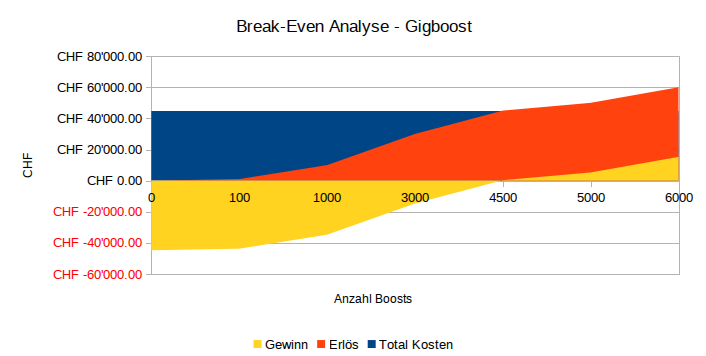
\includegraphics[width=0.95\textwidth]{initialisierung/wirtschaftlichkeit-gigboost.png}
  \caption{Breaz-Even Analyse - Gigboost}
\end{figure}

\clearpage
\subsubsection{Werbung}

Im Modell "Werbung" wird ausgerechnet wieviele aktive Benutzer das Produkt benötigt
um in den nächsten Jahren Gewinn zu erzielen.

Durch Annahme von einem Erlös von \textbf{140.- CHF} pro \textbf{40'0000 Besucher}\footnote{https://www.quora.com/How-much-does-Google-AdSense-pay-for-3-banners-on-a-webpage-per-1-000-views/answer/Manas-Sahu-59} erhalten wir volgendes Bild:

\begin{figure}[!htb]
  \centering
  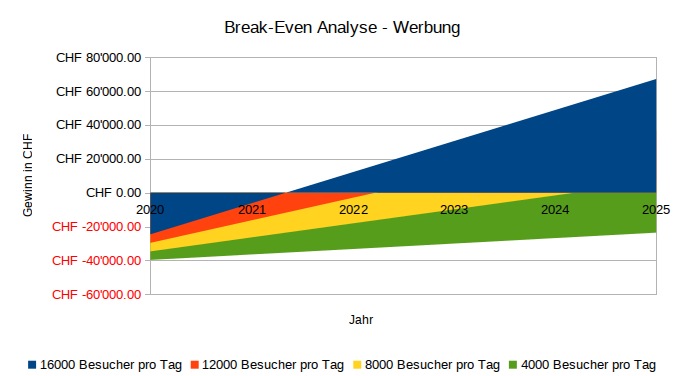
\includegraphics[width=0.95\textwidth]{initialisierung/wirtschaftlichkeit-werbung.png}
  \caption{Break-Even Analyse - Werbung}
\end{figure}

\begin{longtable}[]{@{}lll@{}}
  \toprule
  \textbf{Besucher pro Tag} & \textbf{Erlös pro Tag} & \textbf{Erlös pro Monat}\tabularnewline
  2000                      & 7.- CHF                & 210.- CHF\tabularnewline
  4000                      & 14.- CHF               & 420.- CHF\tabularnewline
  8000                      & 28.- CHF               & 840.- CHF\tabularnewline
  12000                     & 42.- CHF               & 1'260.- CHF\tabularnewline
  16000                     & 46.- CHF               & 1'680.- CHF\tabularnewline
  \bottomrule
  \caption{Werbeeinnahmen pro Besucher}
\end{longtable}

Der Grafik ist zu entnehmen, dass das Produkt bei 8'000 Besucher pro Tag nach ca. 6 Jahren Gewinn erzielt. Bei 12'000 Besucher pro Tag erzielt das Produkt nach bereits 4 Jahren Gewinn und mit 16'000 Beucher pro Tag schon im dritten Jahr.

\chapter{Konzept}

\label{AppendixKonzept}

\section{Zweck des Dokuments}\label{KonzeptZweck}

Das Konzept dient als Anleitung für die Realisierungsphase. Die in der Konzept
erarbeiteten Details müssen in der Realisierung eingehalten un umgesetzt
werden.

\subsection{Teilkonzepte}

Durch die in der Studie gewonnenen Erkentnissen, werden in der Phase Konzept
verschiedene Teilkonzepte erstellt.

Im Teilkonzept «Portalname» wird der Name des Produktes erarbeitet.

Im Teilkonzept «Design- und Bedienkonzept» werden die Ansichten der Applikation
in Mockups umgesetzt. Es werden die Benutzer Use-Cases vom Besucher sowie der
Konzert-Erfasser aufgezeigt.

Im Teilkonzept «Softwarekonzept» werden die Datenflüsse hinter den Mockups
aufgezeigt, sowie die Datenbankstruktur aufgebaut.

Im Teilkonzept «Testkonzept» werden die einzelnen Systemtests aufgelistet sowie
ausgearbeitet wie granular welche Teile der Software getestet werden sollen.

Im letzten Teil des Konzept-Dokuments wird im Fazit dokumentiert, wie und warum
das Konzept von den vorhergehenden Phasen des Projekts abweicht.


\clearpage
\section{Portalname}\label{portalname}

Der Portalname wurde in einer Brainstorming-Session von Damian Senn auf
den Namen \textbf{«Gigpillar»} festgelegt. Der Name ist angelehnt an die Werbepfeiler in
Städten, wo oft Werbeplakate für Konzerte hängen.

Die folgenden Ideen wurden in Betracht gezogen, jedoch war keine Domain mehr
verfügbar oder der Name überzeugte nicht:

\begin{itemize}
  \item{} upto.com («What are you up to?»)
  \item{} up-to.com
  \item{} uptoin.com
  \item{} gigup.com
  \item{} gigsta.com («Gigs to attend»)
  \item{} gigin.com
  \item{} gigsin.com
  \item{} gixin.com («Gigs in»)
  \item{} dualact.com («Loud act»)
  \item{} trecnoc.com («Concert» rückwärts)
\end{itemize}

\clearpage
\section{Design- und Bedienkonzept}\label{design--und-bedienkonzept}

\subsection{Mockups}

\subsubsection{Homepage}

Die Homepage ist die erste Seite, die der Besucher sieht, wenn er/sie die
Applikation direkt über \href{https://gigpillar.com/}{gigpillar.com} aufruft.
Auf den ersten Blick ist die Suche sowie ein grosses Bild (Banner) eines Gigs
zu erblicken. Weiter sind Links zu gängigen Funktionalitäten wie Gig hinzufügen
sowie das Login in einer Navigation erreichbar.

Unter dem Banner werden Gigs in nächster nähe des Besuchers aufgelistet, der
Link «change location» führt weiter zur Suchresultate Seite um den
entsprechenden Filter anzupassen.

\begin{figure}[!htb]
  \centering
  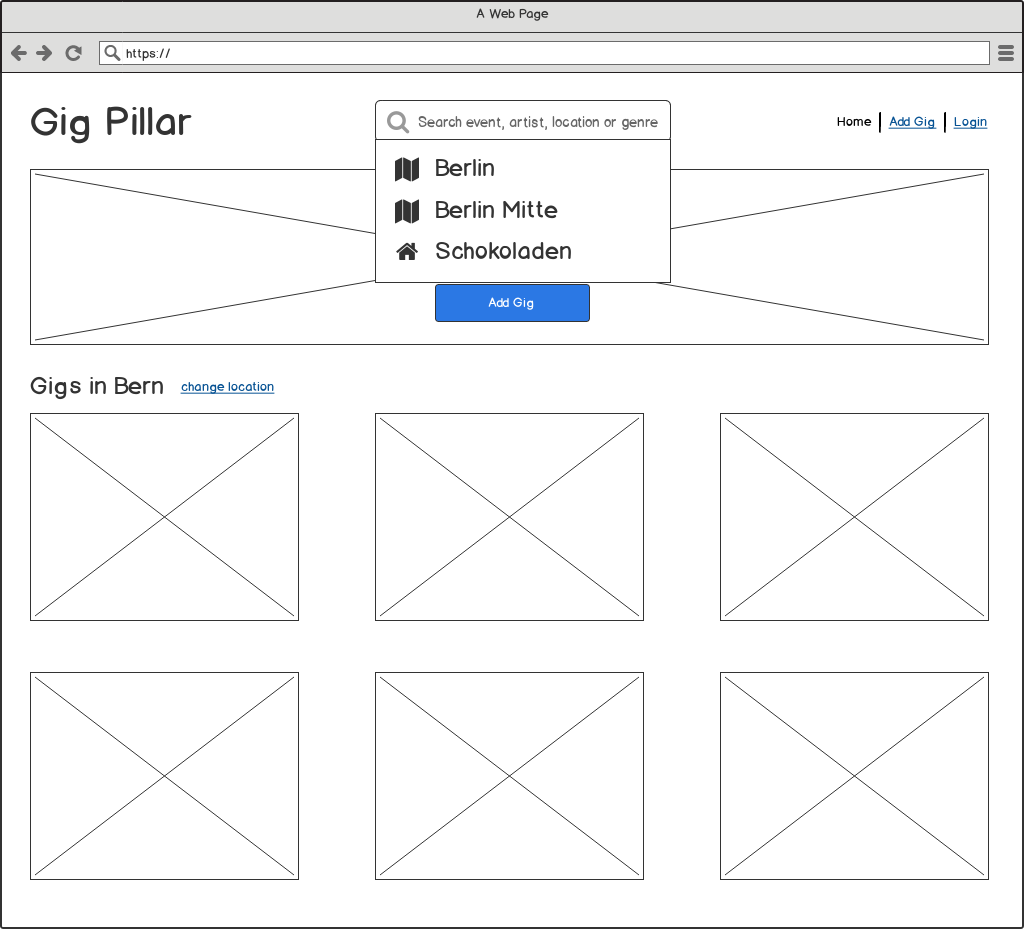
\includegraphics[width=0.95\textwidth]{mockups/homepage.png}
  \caption{Mockup: Homepage}
\end{figure}

\clearpage
\subsubsection{Suchresultate}

Auf der Suchresultate Seite sieht der Benutzer seine Suchresultate der von der
globalen Suchbox ausgelösten Suche. Die Seite bietet weitere Filter an um die
Resultate weiter einzugrenzen.\\

\noindent
Folgende Filter stehen den Benutzern zur Verfügung:

% TODO: This diverges from our search criteria described in the previous phase.

\begin{itemize}
  \tightlist{}
  \item{} Ort
  \item{} Datum von
  \item{} Datum bis
  \item{} Musik Genre
\end{itemize}

\noindent
Das Anwählen eines Suchresultates führt den Benutzer weiter zur detaillierten
Gig Ansicht.

\begin{figure}[!htb]
  \centering
  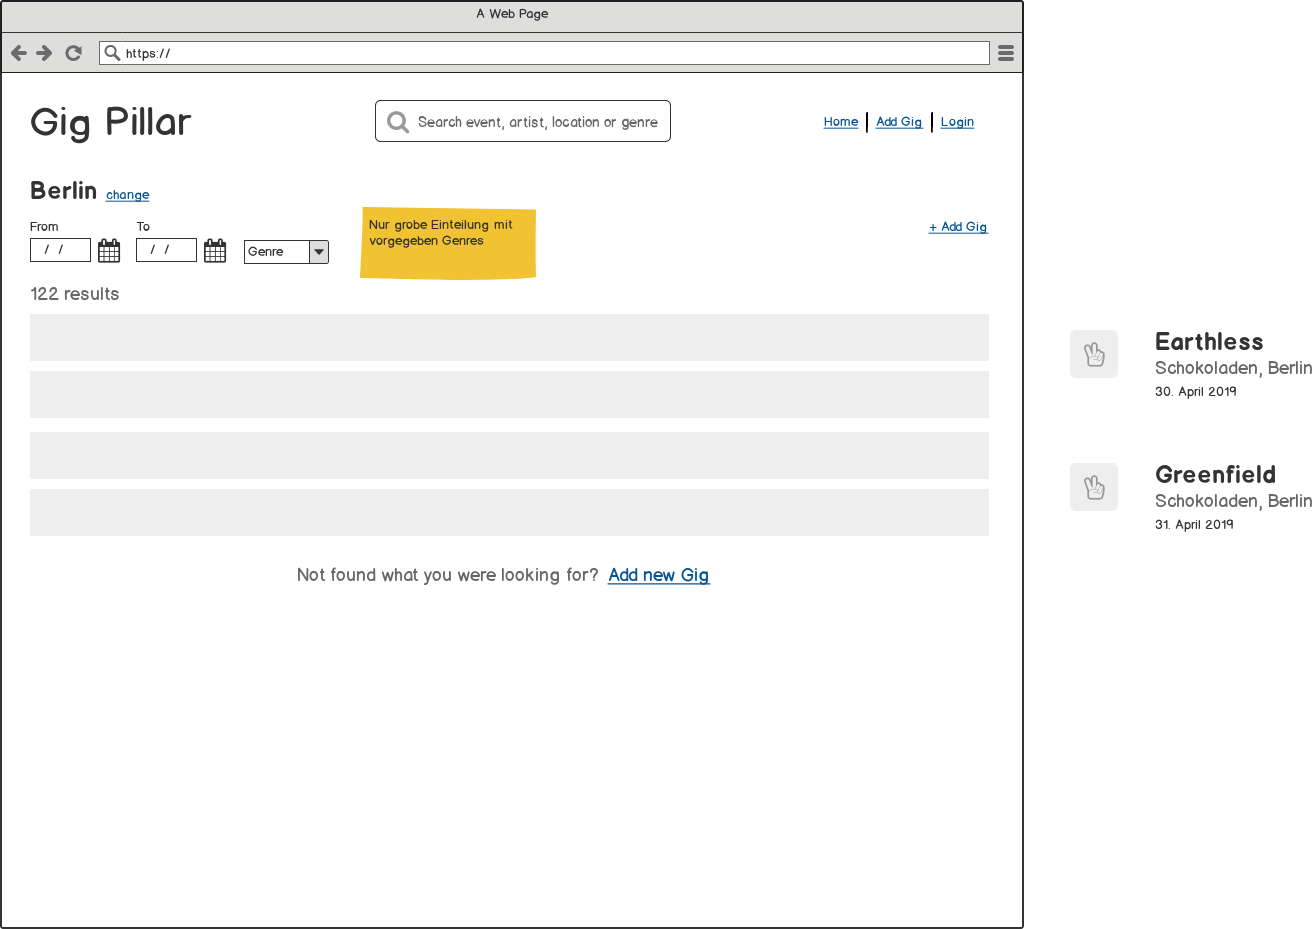
\includegraphics[width=0.95\textwidth]{mockups/search-result.png}
  \caption{Mockup: Suchresultate}
\end{figure}

\clearpage
\subsubsection{Gig Ansicht}

In der Gig Ansicht werden alle Details zu einem Event aufgelistet.

\begin{itemize}
  \tightlist{}
  \item{} Datum des Events
  \item{} Zeit wann das Event beginnt, bzw die Location die Türen öffnet
  \item{} Liste aller Künstler mit optionaler Startzeit
  \item{} Eine Beschreibung des Events
  \item{} Die Adresse der Location mit Link auf Google Maps
\end{itemize}

\noindent
Ausserdem soll es den Benutzern möglich sein, über einen «Add to my calendar»
Link das Event zu seiner Kalender-Applikation zu importieren.

\begin{figure}[!htb]
  \centering
  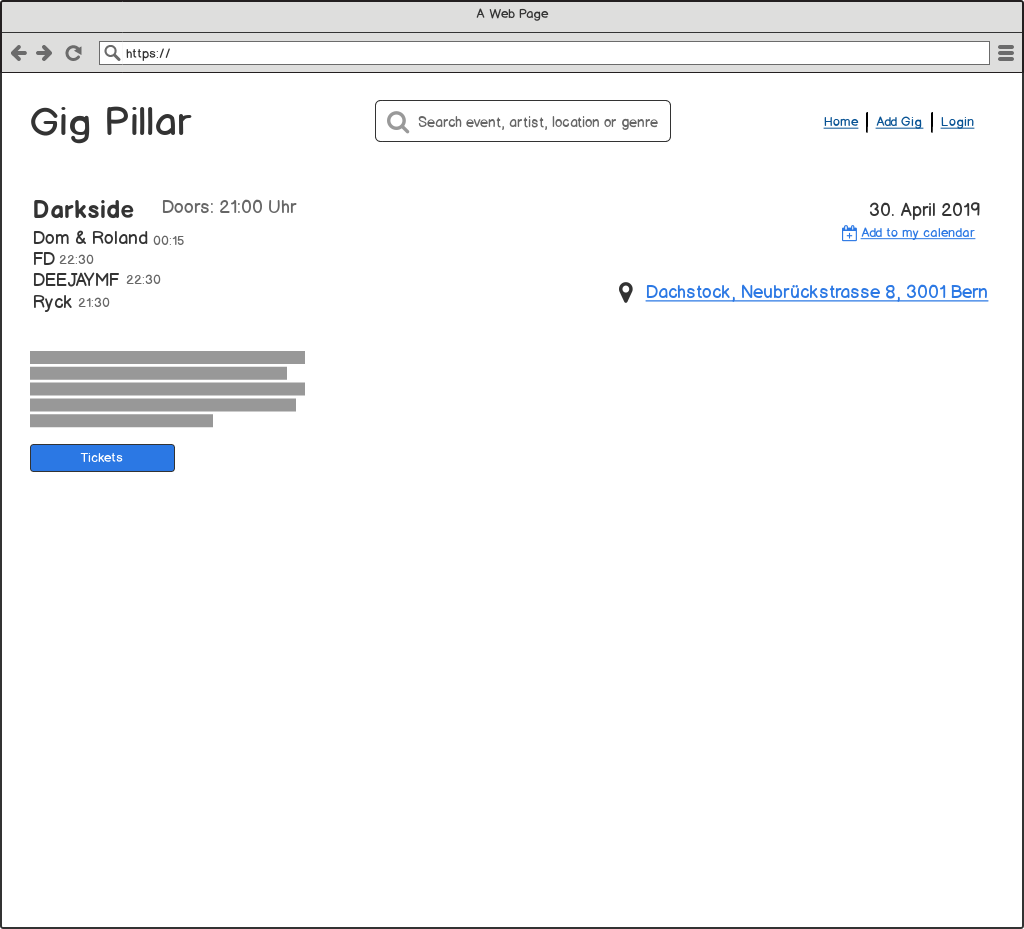
\includegraphics[width=0.95\textwidth]{mockups/event.png}
  \caption{Mockup: Gig Ansicht}
\end{figure}

\clearpage
\subsubsection{Gig erfassen}

Benutzer können Gigs erfassen.\\

\noindent
Folgende Daten sind für einen Gig zu erfassen:

\begin{itemize}
  \tightlist{}
  \item{} Name
  \item{} Bild \textit{(optional)}
  \item{} Location
  \item{} Datum
  \item{} Zeit
  \item{} Eine Liste von Artists mit optionaler Startzeit
  \item{} Beschreibung
  \item{} Link zum Ticketvertreiber
\end{itemize}

\begin{figure}[!htb]
  \centering
  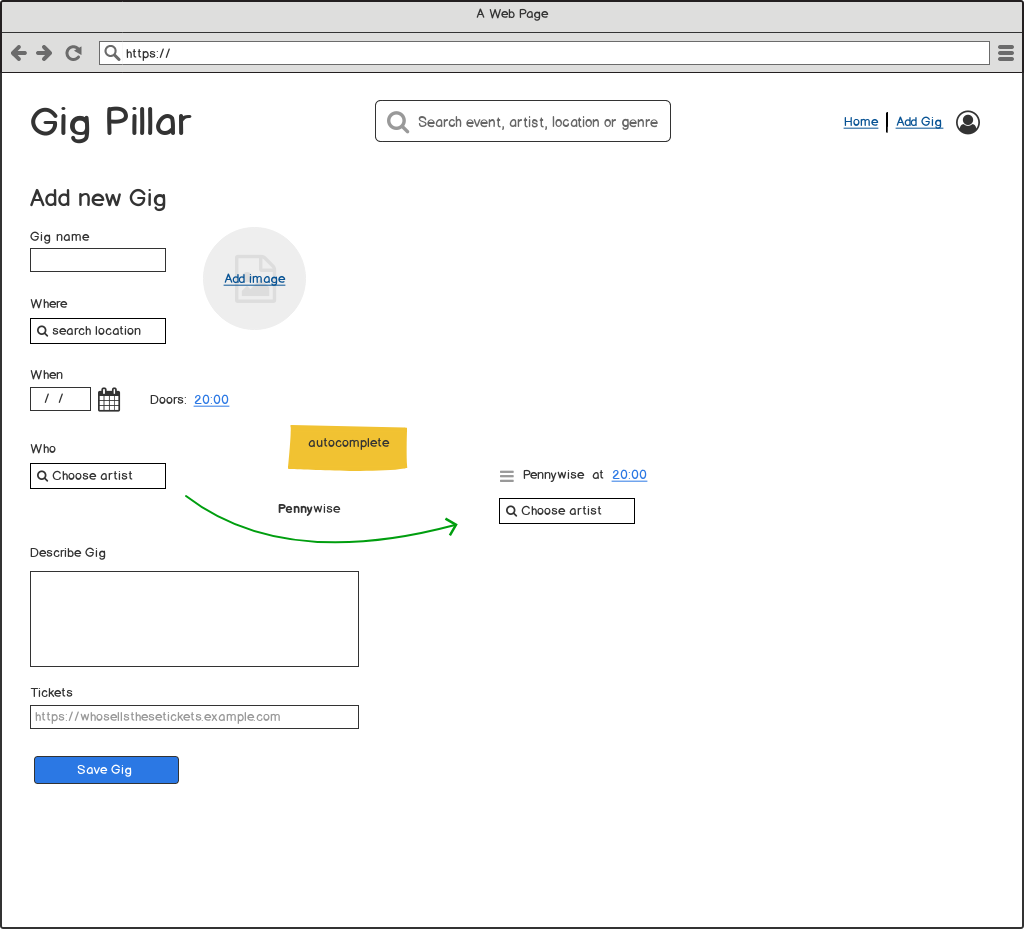
\includegraphics[width=0.95\textwidth]{mockups/add-gig.png}
  \caption{Mockup: Gig erfassen}
\end{figure}

\clearpage
\subsubsection{Benutzerprofil}

Benutzer können ihr eigenes Profil verwalten und folgende Tätigkeiten
verrichten:

\begin{itemize}
  \tightlist{}
  \item{} Anzeigename ändern
  \item{} E-Mail Adresse ändern \textit{(mit E-Mail Bestätigung)}
  \item{} Passwort ändern \textit{(muss vorher altes Passwort bestätigen)}
  \item{} Account löschen \textit{(muss doppelt bestätigt werden!)}
\end{itemize}

\begin{figure}[!htb]
  \centering
  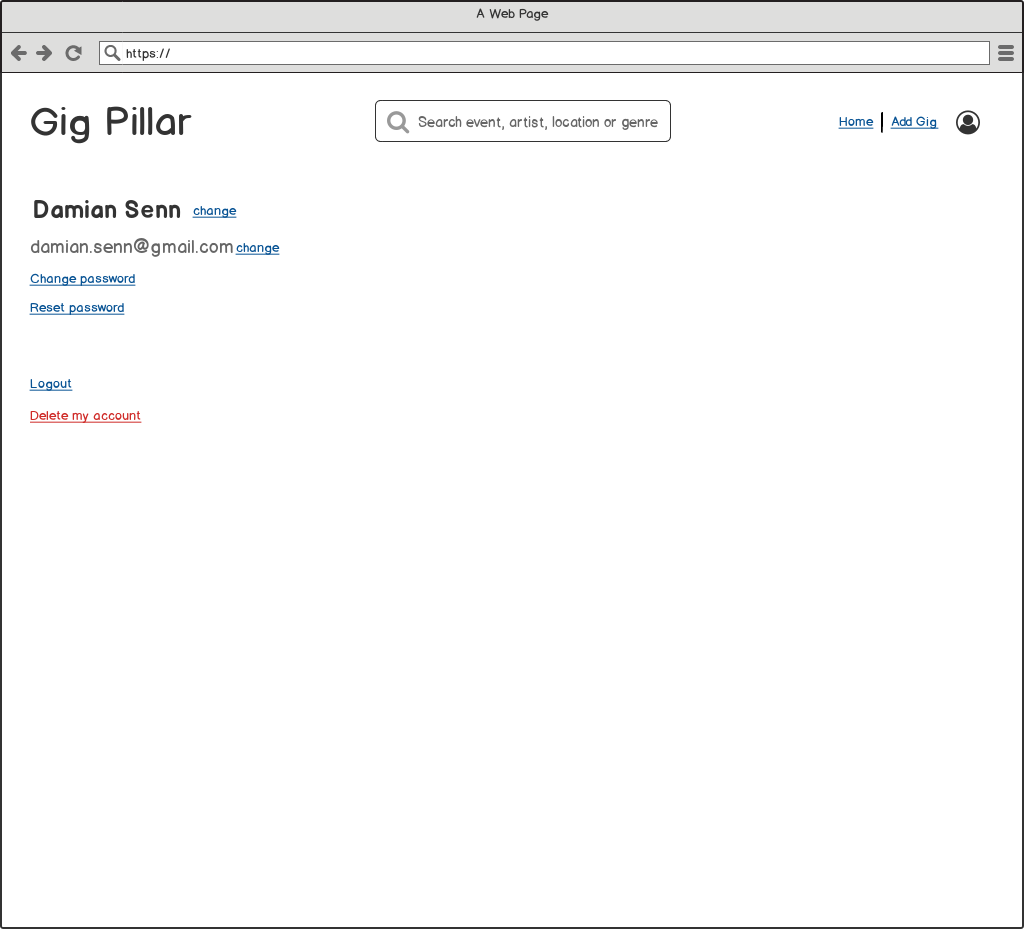
\includegraphics[width=0.95\textwidth]{mockups/profile.png}
  \caption{Mockup: Benutzerprofil}
\end{figure}

\clearpage
\subsection{Genre Filter}\label{genrefilter}

Der Genre Filter soll folgende Werte zur Verfügung stellen.

\begin{itemize}
  \item{} Alternative
  \item{} Blues
  \item{} Classical
  \item{} EDM
  \item{} Hip-Hop
  \item{} Jazz
  \item{} Metal
  \item{} Pop
  \item{} Punk
  \item{} Reggae
  \item{} Rock
\end{itemize}

\clearpage
\section{Softwarekonzept}\label{softwarekonzept}
\subsection{Datenfluss}\label{datenfluss}

\subsubsection{Homepage}\label{datenfluss-homepage}

Die Homepage zeigt den Besuchern Gigs in ihrer Nähe an, dazu muss über eine
GeoIP API die IP-Adresse des Besuchers auf ein Land zurückverfolgt werden.
Dazu wird beim ersten Besuch die GeoIP API abgefragt und das Land des Benutzers
in eine Session geschrieben. Bei weiteren Aufrufen wird das Land direkt aus der
Session bezogen.

%GigPillarWeb
%GigPillarWeb_Session
%GigPillar
%GeoIp
%
%Response = GigPillarWeb./ {
%  if (hasSession) {
%    location = GigPillarWeb_Session.getLocation()
%  } else {
%    location = GigPillarWeb_Session.createSession() {
%      location = GeoIp.getLocation(ip)
%    }
%  }
%
%  Events = GigPillar.getUpcomingEvents(location)
%}

\begin{figure}[!htb]
  \centering
  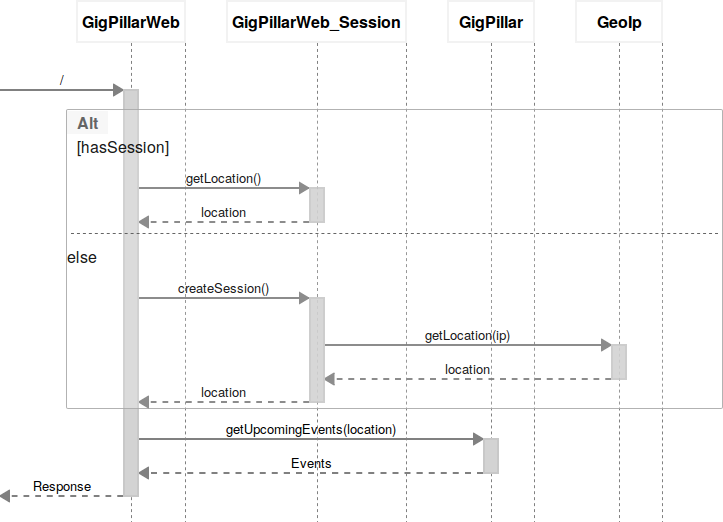
\includegraphics[width=0.95\textwidth]{konzept/datenfluss-homepage.png}
  \caption{Datenfluss: Homepage}
\end{figure}

\clearpage
\subsubsection{Suchfeld}\label{datenfluss-suchfeld}

Das globale Suchfeld hat eine Autocompletion, welche Daten direkt von
der GigPillar Applikation bezieht. Die Daten für Städtenamen wird jedoch von
einer externen Datenquelle, z.B. Google Maps, bezogen.

%GigPillarWeb
%GigPillar
%GoogleMaps
%
%Response = GigPillarWeb./searchCompletion {
%  Cities = GoogleMaps.searchCities(searchParameters)
%  Locations = GigPillar.searchLocations(searchParameters)
%  Genres = GigPillar.searchGenres(searchParameters)
%  Artists = GigPillar.searchArtists(searchParameters)
%  Events = GigPillar.searchEvents(searchParameters)
%}

\begin{figure}[!htb]
  \centering
  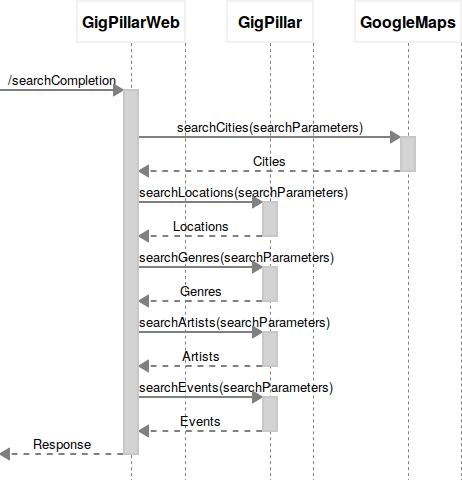
\includegraphics[width=0.95\textwidth]{konzept/datenfluss-suchfeld.png}
  \caption{Datenfluss: Suchfeld}
\end{figure}

\clearpage
\subsubsection{Gig erstellen - Locationfeld}\label{datenfluss-gig-erstellen-locationfeld}

Beim Erstellen eines neuen Gigs, muss eine Location zugewiesen werden. Die
Locations werden über die bereits in GigPillar erfassten Locations sowie über
eine externe Datenquelle, wie z.B. Google Maps, bezogen.

%GigPillarWeb
%GigPillar
%GoogleMaps
%
%Response = GigPillarWeb./locationCompletion {
%  Locations = GigPillar.searchLocations(searchParameters) {
%    Locations = searchLocations(searchParameters)
%    Locations = GoogleMaps.searchLocations(searchParameters)
%  }
%}

\begin{figure}[!htb]
  \centering
  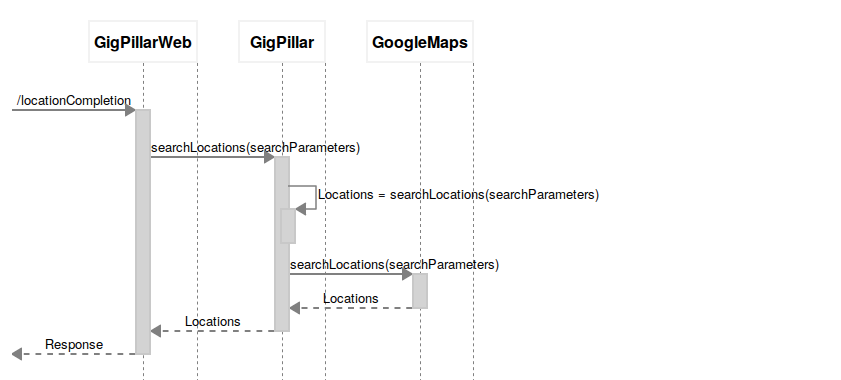
\includegraphics[width=0.95\textwidth]{konzept/datenfluss-locationfeld.png}
  \caption{Datenfluss: Gig erstellen - Locationfeld}
\end{figure}

%TODO:
%\clearpage
%\subsubsection{Gig erstellen}\label{datenfluss-gigerstellen}

\clearpage
\subsubsection{Passwort-Reset}\label{datenfluss-passwort-reset}

Falls ein Benutzer sein Passwort vergessen hat, kann dieser ein neues Passwort
über die Passwort-Reset Funktion setzen. Beim Auslösen eines Passwort-Resets,
wird dem Benutzer ein E-Mail mit einem Link zugeschickt.
Der Passwort-Reset-Link führt den Benutzer auf ein Formular auf welchem er/sie
die Möglichkeit hat, ein neues Passwort zu setzen.

%GigPillarWeb
%GigPillar
%UserEmailClient
%
%Response = GigPillarWeb./passwordReset {
%  GigPillar.sendPasswordResetEmail(email) {
%    GigPillar->UserEmailClient:SMTP
%  }
%}
%
%Redirect = UserEmailClient.clickPasswordResetLink {
%  Response = GigPillarWeb./passwordRestToken
%}
%
%Response = GigPillarWeb./setPassword {
%  GigPillar.setUserPassword(currentUser, password)
%}

\begin{figure}[!htb]
  \centering
  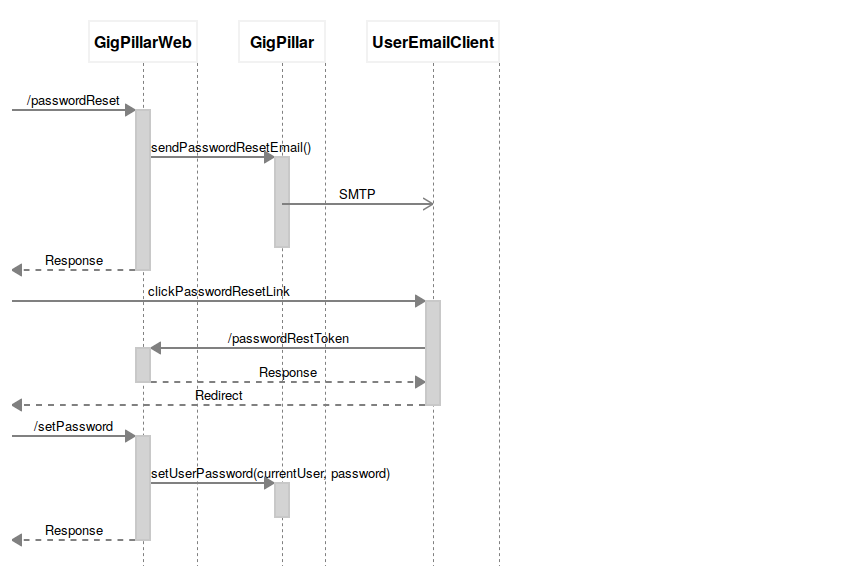
\includegraphics[width=0.95\textwidth]{konzept/datenfluss-passwort-reset.png}
  \caption{Datenfluss: Passwort-Reset}
\end{figure}

\clearpage
\subsection{Datenbankstruktur}\label{datenbankstruktur}

\begin{figure}[!htb]
  \centering
  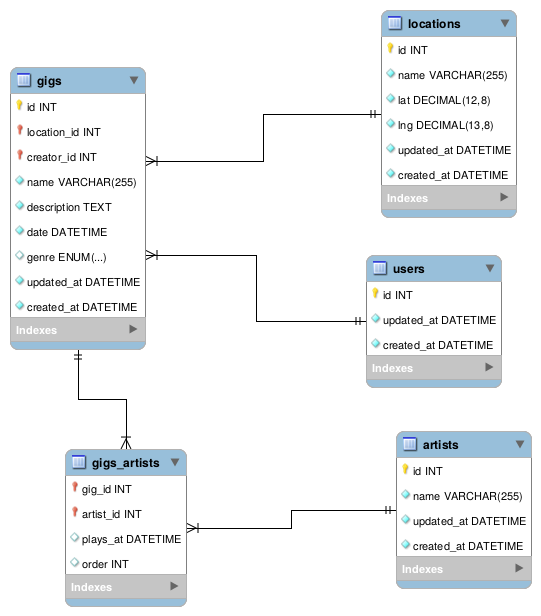
\includegraphics[width=0.95\textwidth]{konzept/erd.png}
  \caption{Entity Relationship Diagram}
\end{figure}

\clearpage
\section{Testkonzept}\label{testkonzept}

\subsection{Unit-Tests}\label{unittests}

% Do ~80% code coverage

\subsection{Visual-Tests}\label{visualtests}

% Do simple screenshot diffing for every screen

\clearpage
\subsection{Akzeptanztests}\label{akzeptanztests}

% TODO: Akzeptanztest basieren auf Anforderungen

\newcounter{acceptancetest}

\NewDocumentCommand{\acceptancetest}{
  O{}
  O{}
  O{\tabularnewline\tabularnewline}
  O{\tabularnewline\tabularnewline\tabularnewline\tabularnewline}
  m
  m
}{
  \begin{longtable}[]{@{}l|p{6cm}p{4cm}@{}}
    \toprule
    \stepcounter{acceptancetest}
    \textbf{Test \arabic{acceptancetest}} & \textbf{Tester:} #1 & \textbf{Datum:} #2 \tabularnewline
    \midrule
    \textbf{Kriterium}                    & \multicolumn{2}{p{10cm}}{#5}\tabularnewline
    \textbf{Erwartetes Ergebnis}          & \multicolumn{2}{p{10cm}}{#6}\tabularnewline
    \midrule
    \textbf{Testergebnis}                 & #3\tabularnewline
    \midrule
    \textbf{Fehlerbeschreibung}           & #4\tabularnewline
    \bottomrule
    \caption{Akzeptanztest \arabic{acceptancetest}}
  \end{longtable}
}

\acceptancetest
  {Es ist möglich nach Konzerten in einem bestimmten Ort zu suchen.}
  {Nach auswählen von «Berlin» in der Suche, werden nur noch Konzerte in Berlin aufgelistet.}

\acceptancetest
  {Es ist möglich eine Suche weiter nach Genre einzuschränken.}
  {Nach auswählen von «Rock» in einem Suchresultat, werden nur noch Rock-Konzerte aufgelistet.}

\clearpage

\acceptancetest
  {Responsive - Homepage}
  {Sieht auf Desktop, Tablet und Mobile gut aus und stellt jeweils alle relevanten Daten dar.}

\acceptancetest
  {Browserkompatibilität - Homepage}
  {Funktioniert in den unterstützten Browsern.}

\clearpage

\acceptancetest
  {Responsive - Suche}
  {Sieht auf Desktop, Tablet und Mobile gut aus und stellt jeweils alle relevanten Daten dar.}

\acceptancetest
  {Browserkompatibilität - Suche}
  {Funktioniert in den unterstützten Browsern.}

\clearpage

\acceptancetest
  {Responsive - Gig Ansicht}
  {Sieht auf Desktop, Tablet und Mobile gut aus und stellt jeweils alle relevanten Daten dar.}

\acceptancetest
  {Browserkompatibilität - Gig Ansicht}
  {Funktioniert in den unterstützten Browsern.}

\clearpage

\acceptancetest
  {Responsive - Login}
  {Sieht auf Desktop, Tablet und Mobile gut aus und stellt jeweils alle relevanten Daten dar.}

\acceptancetest
  {Browserkompatibilität - Login}
  {Funktioniert in den unterstützten Browsern.}

\clearpage

\acceptancetest
  {Responsive - Registrierung}
  {Sieht auf Desktop, Tablet und Mobile gut aus und stellt jeweils alle relevanten Daten dar.}

\acceptancetest
  {Browserkompatibilität - Registrierung}
  {Funktioniert in den unterstützten Browsern.}

\clearpage

\acceptancetest
  {Responsive - Gig erfassen}
  {Sieht auf Desktop, Tablet und Mobile gut aus und stellt jeweils alle relevanten Daten dar.}

\acceptancetest
  {Browserkompatibilität - Gig erfassen}
  {Funktioniert in den unterstützten Browsern.}

\clearpage

\acceptancetest
  {Gig erfassen}
  {Folgende Daten können erfasst werden:
  \begin{itemize}
    \tightlist{}
    \item{} Name
    \item{} Bild
    \item{} Location
    \item{} Datum
    \item{} Zeit
    \item{} Künstler mit optinaler Start-Zeit
    \item{} Beschreibung
    \item{} Link zum Ticketvertreiber
  \end{itemize}}

\acceptancetest
  {Neue Gigs tauchen in der Suche auf.}
  {Der neu erstellte Gig taucht in der Suche auf.}

\clearpage

\acceptancetest
  {Responsive - Benutzerprofil}
  {Sieht auf Desktop, Tablet und Mobile gut aus und stellt jeweils alle relevanten Daten dar.}

\acceptancetest
  {Browserkompatibilität - Benutzerprofil}
  {Funktioniert in den unterstützten Browsern.}

\clearpage

\acceptancetest
  {Responsive - Passwort-Reset}
  {Sieht auf Desktop, Tablet und Mobile gut aus und stellt jeweils alle relevanten Daten dar.}

\acceptancetest
  {Browserkompatibilität - Passwort-Reset}
  {Funktioniert in den unterstützten Browsern.}

\clearpage

\acceptancetest
  {Security - Suche}
  {Das Suchfeld ist resistent gegen XSS und SQL-Injection}

\acceptancetest
  {Security - Login}
  {Das Login ist resistent gegen XSS und SQL-Injection}

\clearpage

\acceptancetest
  {Security - Benutzerprofil}
  {Das Benutzerprofil ist resistent gegen XSS und SQL-Injection}

\acceptancetest
  {Security - Gig erfassen}
  {Das Gig erfassen Formular ist resistent gegen XSS und SQL-Injection}

\clearpage
\section{Fazit}\label{konzept-fazit}

\subsection{Probleme}

% Abweichung "Filter-System" in Suche?

\subsection{Machbarkeit}

% Google Maps API?

\subsection{Wirtschaftlichkeit}

% Änderung an Aufwand?

\subsection{Erweiterbarkeit}

% FB Events etc?

\subsection{Projektplan}

\chapter{Arbeitsjournal}

\label{AppendixArbeitsjournal}

\section{Sonntag 3. März}\label{sonntag-3.-muxe4rz}

2h:

\begin{itemize}
  \tightlist
  \item
        Vorbereitung Kick-off
  \item
        Abgrenzung erweitern
  \item
        Grobe Anforderungen
  \item
        Auflistung möglicher Variantenentscheide
  \item
        TODO ergänzt
\end{itemize}

\section{Dienstag 5. März}\label{dienstag-5.muxe4rz}

2h:

\begin{itemize}
  \tightlist
  \item
        Vorbereitung Kick-off
\end{itemize}

\section{Mittwoch 6. März}\label{mittwoch-6.muxe4rz}

3h:

\begin{itemize}
  \tightlist
  \item
        Vorbereitung Sitzungszimmer
  \item
        Kick-off Meeting
\end{itemize}

4h:

\begin{itemize}
  \tightlist
  \item
        An Projektauftrag arbeiten - Auftraggeber geändert nach Empfehlung
        von Marc Aeby
\end{itemize}

\section{Samstag 9. März}\label{samstag-9.muxe4rz}

2h:

\begin{itemize}
  \tightlist
  \item
        An Studie/Pflichtenheft arbeiten
\end{itemize}

\section{Dienstag 12. März}\label{dienstag-12.muxe4rz}

2h:

\begin{itemize}
  \tightlist
  \item
        PDF Generierung und Ordnerstruktur angepasst
\end{itemize}

\section{Samstag 16. März}\label{samstag-16.muxe4rz}

3h:

\begin{itemize}
  \tightlist
  \item
        Projektplan von gantt nach ods migrieren
\end{itemize}

\section{Dienstag 19. März}\label{dienstag-19.muxe4rz}

0.5h:

\begin{itemize}
  \tightlist
  \item
        Projektplan in Berichtanhang angehängt
\end{itemize}

\section{Mittwoch 27. März}\label{mittwoch-27.muxe4rz}

1.5h:

\begin{itemize}
  \tightlist
  \item
        Projektplan an korrekte HERMES 5 Struktur angepasst
  \item
        Titelblatt von Ilias hinzugefügt
  \item
        Termin am 12.04.2019 mit Joshua Schär für einen Screendesign-Workshop abgemacht
\end{itemize}

\section{Sonntag 31. März}\label{sonntag-31.muxe4rz}

5h:

\begin{itemize}
  \tightlist
  \item
        Projektziele erweitert
  \item
        Anforderungskatalog erweitert
\end{itemize}

\section{Sonntag 31. März}\label{sonntag-31.muxe4rz}

8h:

\begin{itemize}
  \tightlist
  \item
        Definitive Projektziele definiert
  \item
        Anforderungskatalog fertig gestellt
  \item
        Gesamte Berichtstruktur ausgelegt, Ziele und Abgrenzungen in Bericht
        hinterlegt und referenziert
\end{itemize}

\section{Freitag 5. April}\label{freitag-5.april}

2h:

\begin{itemize}
  \tightlist
  \item
        An Studie weiter gearbeitet
  \item
        Variantenkriterien definiert
\end{itemize}

\section{Samstag 6. April}\label{samstag-6.april}

4h:

\begin{itemize}
  \tightlist
  \item
        An Studie weiter gearbeitet
  \item
        Variantenbeschreibungen erstellt
  \item
        Variantenbewertungen
\end{itemize}

\section{Mittwoch 10. April}\label{mittwoch-10.april}

2h:

\begin{itemize}
  \tightlist
  \item
        Brainstorming für Portalnamen
\end{itemize}

\section{Freitag 12. April}\label{freitag-12.april}

12h:

\begin{itemize}
  \tightlist
  \item
        Screens definiert
  \item
        Mit Joshua Schär an Mockups gearbeitet
\end{itemize}

\section{Samstag 13. April}\label{samstag-13.april}

12h:

\begin{itemize}
  \tightlist
  \item
        Risiko Management
  \item
        Variantenbeschreibungen angepasst/erweitert
  \item
        Projektauftrag
\end{itemize}

\section{Sonntag 14. April}\label{sonntag-14.april}

8h:

\begin{itemize}
  \tightlist
  \item
        Wirtschaftlichkeit
  \item
        Projektauftrag
\end{itemize}

\section{Montag 15. April}\label{montag-15.april}

2h:

\begin{itemize}
  \tightlist
  \item
        Initiales Datenbankschema basierend auf Mockups
\end{itemize}

\section{Mittwoch 17. April}\label{mittwoch-17.april}

0.5h:

\begin{itemize}
  \tightlist
  \item
        Zwischen-Meeting in Planung in richtiger KW eingetragen.
  \item
        Biweekly Reports in Anhang eingefügt.
\end{itemize}

\section{Freitag 19. April}\label{freitag-19.april}

10h:

\begin{itemize}
  \tightlist
  \item
        Alle Mockups detailreicher beschrieben.
  \item
        Kleinere Mockup Anpassungen.
  \item
        Software Konzept mit Datenfluss-Charts beschrieben
\end{itemize}

\section{Sonntag 21. April}\label{sonntag-21.april}

10h:

\begin{itemize}
  \tightlist
  \item
        Mockup Beschreibungen
  \item
        Datenbankschema
  \item
        Mit Testkonzept begonnen
\end{itemize}

\section{Montag 22. April}\label{montag-22.april}

2h:

\begin{itemize}
  \tightlist
  \item
        An Testkonzept gearbeitet
  \item
        An Datenbankschema gearbeitet
\end{itemize}

\section{Dienstag 23. April}\label{dienstag-23.april}

6h:

\begin{itemize}
  \tightlist
  \item
        Zwischenmeeting Präsentation erstellt
  \item
        An Datenbankschema gearbeitet
\end{itemize}

\section{Mittwoch 24. April}\label{mittwoch-24.april}

3h:

\begin{itemize}
  \tightlist
  \item
        Zwischenmeeting
  \item
        Initiales Projektsetup erstellt
\end{itemize}

\section{Mittwoch 1. Mai}\label{mittwoch-1.mai}

14h:

\begin{itemize}
  \tightlist
  \item
        Begin an HTML-Prototypen
\end{itemize}

\section{Sonntag 5. Mai}\label{sonntag-5.mai}

11h:

\begin{itemize}
  \tightlist
  \item
        An HTML-Prototypen gearbeitet
  \item
        Initiale Login Implementation
\end{itemize}

\section{Montag 6. Mai}\label{montag-6.mai}

12h:

\begin{itemize}
  \tightlist
  \item
        Script zum erstellen von Benutzern
  \item
        Registrierungsprozess implementiert
  \item
        Session Management eingerichtet
  \item
        Berechtigungssystem definiert
  \item
        Mit Erfassungsformular für Gigs begonnen
\end{itemize}

\section{Dienstag 7. Mai}\label{dienstag-7.mai}

1h:

\begin{itemize}
  \tightlist
  \item
        Unit-Tests für Gigs
\end{itemize}

\section{Mittwoch 8. Mai}\label{mittwoch-8.mai}

10h:

\begin{itemize}
  \tightlist
  \item
        An Gig Erfassungsformular gearbeitet, diverse Problematiken mit
        Phoenix Formular sowie Datenbankbeziehungen aufgetreten.
  \item
        Google Places API angebunden für Location Autocomplete
  \item
        Generische Suchbox in HTML/JavaScript implementiert
\end{itemize}

\section{Donnerstag 9. Mai}\label{donnerstag-9.mai}

11h:

\begin{itemize}
  \tightlist
  \item
        JavaScript, HTML und CSS Optimierungsplugins installiert
  \item
        Location Autocomplete fertiggestellt
  \item
        Künstlerfeld für Gigs implementiert
  \item
        Fehlermeldungen für invalide Felder eingefügt
  \item
        Bildinputfeld implementiert
  \item
        Debugging von diversen Probleme im Zusammenhang mit Datenbankrelationen
        für das Gig erfassen/updaten Formular
\end{itemize}

\section{Freitag 10. Mai}\label{freitag-10.mai}

1h:

\begin{itemize}
  \tightlist
  \item
        Dropdown Element implementiert
\end{itemize}

\section{Samstag 11. Mai}\label{samstag-11.mai}

13h:

\begin{itemize}
  \tightlist
  \item
        Dropdown Element implementiert
  \item
        Debugging von diversen Probleme im Zusammenhang mit Datenbankrelationen
        für das Gig erfassen/updaten Formular
\end{itemize}

\section{Sonntag 12. Mai}\label{sonntag-12.mai}

7h:

\begin{itemize}
  \tightlist
  \item
        Bildupload für Gigs
  \item
        Begin der Implementation der Suche
\end{itemize}

\section{Montag 13. Mai}\label{montag-13.mai}

10h:

\begin{itemize}
  \tightlist
  \item
        Bilder resizing für Gigs
  \item
        Besucher Location mit GeoIP auflösen
  \item
        Diverse kleinere Bugfixes
  \item
        Gig-Detail Ansicht implementiert
\end{itemize}

\section{Dienstag 14. Mai}\label{dienstag-14.mai}

14h:

\begin{itemize}
  \tightlist
  \item
        Browser-Tests für Gig erstellen, Registrierung, Login und Suche
  \item
        Location Autocomplete Sessiontoken hinzugefügt
  \item
        Realisierungsdokumentation
\end{itemize}

\section{Mittwoch 15. Mai}\label{mittwoch-15.mai}

15h:

\begin{itemize}
  \tightlist
  \item
        Realisierungsdokumentation
  \item
        Bericht schreiben
\end{itemize}


%------------------------------------------------------------------------------
% BIBLIOGRAPHY
%------------------------------------------------------------------------------

\printbibliography[heading=bibintoc]

%------------------------------------------------------------------------------

\end{document}
